%% Dokumentenklasse (KOMA-Script) ==========================================
%% scrreprt: Report-Klasse mit Chaptern, ideal für Abschlussarbeiten
\documentclass[%
   final,%              % Finales Dokument (vs. draft)
   paper=a4,%           % DIN A4 Papierformat
   pagesize=auto,%      % PDF-Seitengröße automatisch einstellen
   fontsize=12pt,%      % [IU-FIX] 12pt Latin Modern ≈ visuelles Äquivalent zu Arial 11pt
   version=last%        % Neueste KOMA-Script Version
]{scrreprt}
 
 
%% Spracheinstellung ========================================================
\def\lang{ngerman}
 
%% KI-Tools Declaration (erforderlich bei KI-Nutzung) =======================
\def\declareUseOfGenerativeAITool{GitHub Copilot, ChatGPT~5.2, Google Gemini~3.1, Elicit, Consensus}
 
%% Preambel laden ===========================================================
%%% ========================================================================
%%% KOMA-Script Settings (settings.tex)
%%% 
%%% IU-Konformität: Änderungen gemäß "Richtlinien für die Gestaltung
%%% wissenschaftlicher Arbeiten an der IU" (Stand 01.10.2025)
%%% sind mit "% [IU-FIX]" markiert.
%%% ========================================================================
 
%%% === Seitenlayout ===========================================================
%%% [IU-FIX] twoside=false: IU verlangt einseitigen Druck
%%% (vorher: twoside=true)
%%% [IU-FIX] DIV und BCOR entfernt – Ränder werden über geometry gesteuert
%%% (vorher: DIV=11, BCOR=5mm → kollidierte mit geometry-Rändern)
\KOMAoptions{%
   twoside=false,%         % [IU-FIX] Einseitig (IU: "einseitig zu beschreiben")
   twocolumn=false,%       % Einspaltig
   headinclude=false,%      % [IU-FIX] Kopfzeile im Satzspiegel berücksichtigen
   footinclude=true,%      % [IU-FIX] Fußzeile im Satzspiegel berücksichtigen
   headsepline=false,%      % Linie unter Kopfzeile
   cleardoublepage=empty%
}%
 
%%% === Überschriften ==========================================================
\KOMAoptions{%
   headings=big,%             % Große Überschriften mit viel Abstand
   headings=noappendixprefix,% Keine speziellen Anhang-Präfixe
   headings=nochapterprefix,%  % Keine Nummern-Präfixe bei Kapiteln
   numbers=noenddot%           % Kein Punkt nach Kapitelnummern
}%
%%% [IU-FIX] headings=openright entfernt – bei einseitigem Druck irrelevant
%%% und kann zu leeren Seiten führen
\setcounter{secnumdepth}{3}
 
%%% === Table of Contents =====================================================
\setcounter{tocdepth}{3}
\KOMAoptions{%
   toc=indented,%
   toc=bib,%
   toc=noindex,%
   toc=nolistof%
}%
 
%%% === Lists of figures, tables etc. =========================================
\KOMAoptions{%
   listof=indented,%
   listof=chaptergapsmall,%
   listof=totoc%
}%
 
%%% === Bibliography ==========================================================
\KOMAoptions{%
   bibliography=openstyle,%
   bibliography=totoc%
}%
 
%%% === Index =================================================================
\KOMAoptions{%
   index=nottotoc%
}%
 
%%% === Titlepage =============================================================
\KOMAoptions{%
   titlepage=true%
}%
 
%%% === Miscellaneous =========================================================
\KOMAoptions{%
   footnotes=multiple%
}%
%%% ----------------------------------------------------------------------
%%% LaTeX-Präambel
%%% Hier werden alle Pakete geladen und Einstellungen vorgenommen.
%%%
%%% IU-Konformität: Anpassungen gemäß "Richtlinien für die Gestaltung
%%% wissenschaftlicher Arbeiten an der IU" (Stand 01.10.2025) sind mit
%%% dem Kommentar "% [IU-FIX]" gekennzeichnet.
%%% ----------------------------------------------------------------------
 
%%% 1. Basiskonfiguration & Hilfsbefehle
%%% ----------------------------------------------------------------------
\input{preambel/preambel-commands}
 
%%% Spracheinstellungen (Babel)
\ifthenelse{\equal{\lang}{ngerman}}
  {\usepackage[ngerman]{babel}}
  {\usepackage[english]{babel}}
 
%%% Farben
\usepackage[table]{xcolor}
 
%%% Bilder einbinden
\usepackage{graphicx}
 
%%% Querformat für einzelne Seiten
\usepackage{pdflscape}
 
%%% Rechnen mit LaTeX (wird oft intern benötigt)
\usepackage{calc}
 
 
%%% 2. Text & Typografie
%%% ----------------------------------------------------------------------
 
%%% Schrift-Encoding und Symbole
\usepackage[T1]{fontenc}
\usepackage{textcomp}
 
%%% Schriftarten laden (ausgelagert)
%%% [IU-HINWEIS] Die IU verlangt Arial oder eine vergleichbare serifenlose
%%% Schriftart. Stelle sicher, dass preambel/Fonts eine solche setzt,
%%% z.B. \usepackage{helvet}\renewcommand{\familydefault}{\sfdefault}
\input{preambel/Fonts}
 
%%% Zeilenabstand (1,5-fach) – [IU-konform: "1,5-zeiliger Abstand"]
\usepackage{setspace}
\onehalfspacing
 
%%% Absatzlayout – [IU-FIX] Kein Einzug, 6 Pt. Abstand nach Absatz
\setlength{\parindent}{0pt}
\setlength{\parskip}{6pt plus 1pt minus 1pt}% [IU-FIX] exakt 6pt
 
%%% Überschriften-Abstände gemäß IU-Richtlinie
%%% [IU-FIX] 1. Stufe: 12 Pt. vor und 12 Pt. nach
%%% [IU-FIX] 2. und 3. Stufe: 12 Pt. vor, 6 Pt. nach
\RedeclareSectionCommand[
  beforeskip=12pt,
  afterskip=12pt
]{chapter}
\RedeclareSectionCommand[
  beforeskip=12pt,
  afterskip=6pt
]{section}
\RedeclareSectionCommand[
  beforeskip=12pt,
  afterskip=6pt
]{subsection}
\RedeclareSectionCommand[
	beforeskip=6pt,
	afterskip=-0.5em
]{paragraph}
 
%%% Mikrotypografie (Optischer Randausgleich etc.)
\usepackage[
   protrusion=true
]{microtype}
 
\emergencystretch=2em
 
%%% Besserer Flattersatz (nur für Überschriften/Verzeichnisse, nicht global)
\usepackage{ragged2e}
 
%%% Intelligente "..." (\dots)
\usepackage{ellipsis}
 
%%% Textauszeichnungen
\usepackage[normalem]{ulem}
\usepackage{soul}
 
%%% URLs korrekt umbrechen
\usepackage{xurl}
 
%%% Anführungszeichen (passend zur Sprache)
\usepackage[babel, german=quotes, english=british, french=guillemets]{csquotes}
\SetBlockThreshold{2}
 
 
%%% 3. Layout & Seitenränder
%%% ----------------------------------------------------------------------
 
%%% [IU-FIX] Seitenränder 2,00 cm – mit Platz für Kopf- und Fußzeile
%%% Die IU verlangt 2 cm Rand auf allen Seiten. Da Kopf- und Fußzeile
%%% innerhalb des Satzspiegels liegen (headinclude=true, footinclude=true
%%% in settings.tex), definieren wir den Textbereich so, dass der
%%% sichtbare Rand zum Papierrand exakt 2 cm beträgt.
%%% includehead/includefoot sorgt dafür, dass geometry den Platz für
%%% Header/Footer aus dem Textbereich herausrechnet, nicht aus dem Rand.
\usepackage[
  top=2cm,
  bottom=2cm,
  left=2cm,
  right=2cm,
  includefoot,          % [IU-FIX] Fußzeile innerhalb des 2cm-Rands platzieren
  headheight=14pt,      % Höhe der Kopfzeile (passend für 10pt Schrift + Linie)
  headsep=8pt,          % Abstand Kopfzeile → Textbeginn
  footskip=20pt         % Abstand Textende → Seitenzahl
]{geometry}
 
%%% Kopf- und Fußzeilen (KOMA-Script)
\usepackage[
   automark,
   pagestyleset=KOMA-Script,
   markcase=ignoreuppercase,
]{scrlayer-scrpage}
 
\raggedbottom
 
% Standard-Stile löschen
\clearmainofpairofpagestyles
\clearplainofpairofpagestyles
 
% Kopfzeile deaktivieren
\ohead{}
 
% [IU-FIX] Seitenzahlen zentriert am Seitenende
\cfoot[\pagemark]{\pagemark}
 
% Obere Leiste (Linie) deaktivieren
\KOMAoptions{headsepline=false}
 
% Breite von Kopf/Fuß an Text anpassen
\KOMAoptions{headwidth=text:0pt, footwidth=text:0pt}
 
% Schriftart für Kopf/Fuß
\setkomafont{pageheadfoot}{\normalfont\normalcolor\small\sffamily}
\setkomafont{pagenumber}{\bfseries\sffamily}
 
%%% Fußnoten
\usepackage[bottom, stable, multiple]{footmisc}
\deffootnote{1.5em}{1em}{\makebox[1.5em][l]{\thefootnotemark}}
\addtolength{\skip\footins}{\baselineskip}
 
%%% Einzelne Zeilen am Seitenanfang/-ende vermeiden
\clubpenalty=3000
\widowpenalty=3000
\displaywidowpenalty=2000
 
 
%%% 4. Tabellen & Abbildungen
%%% ----------------------------------------------------------------------
 
\usepackage{booktabs}
\usepackage{multirow}
\usepackage{dcolumn}
\usepackage{ltxtable}
\usepackage{tabularx}
\usepackage{array}
\usepackage{colortbl}
 
\definecolor{rowcolorgray}{gray}{0.90}
\definecolor{headercolor}{RGB}{120,150,180}
 
\newcolumntype{L}[1]{>{\raggedright\let\newline\\\arraybackslash\hspace{0pt}}m{#1}}
\newcolumntype{C}[1]{>{\centering\let\newline\\\arraybackslash\hspace{0pt}}m{#1}}
\newcolumntype{R}[1]{>{\raggedleft\let\newline\\\arraybackslash\hspace{0pt}}m{#1}}
\newcolumntype{S}{>{\centering\arraybackslash}p{0.5cm}}
 
\renewcommand{\arraystretch}{1.5}
\setlength{\tabcolsep}{8pt}
 
\usepackage{float}
\usepackage{flafter}
\usepackage[section]{placeins}
 
\usepackage{subcaption}
 
\usepackage{tikz}
\usetikzlibrary{arrows.meta,positioning,shapes,fit}
 
\usepackage{wrapfig}
\setlength{\intextsep}{0.5\baselineskip}
 
\usepackage{caption}
\captionsetup{
   margin = 10pt,
   font = {small,rm},
   labelfont = {small,bf},
   format = plain,
   indention = 0em,
   labelsep = colon,
   justification = RaggedRight,
   singlelinecheck = true,
   position = bottom
}
\DeclareCaptionOption{parskip}[]{}
\DeclareCaptionOption{parindent}[]{}
 
\usepackage{capt-of}
 
\usepackage[most]{tcolorbox}
 
 
%%% 5. Mathematik & Wissenschaft
%%% ----------------------------------------------------------------------
 
\usepackage{amsmath}
\usepackage[fixamsmath,disallowspaces]{mathtools}
 
\usepackage{fixmath}
 
\usepackage{icomma}
 
\usepackage{siunitx}
\sisetup{
	detect-all = true,
	locale = DE,
	per-mode = symbol
}
\newcommand{\pct}[1]{\SI{#1}{\percent}}
 
\usepackage{braket}
\usepackage{cancel}
\usepackage{empheq}
\usepackage{pifont}
\usepackage[Symbolsmallscale]{upgreek}
\usepackage[upmu]{gensymb}
 
\let\ORGvarepsilon=\varepsilon
\let\varepsilon=\epsilon
\let\epsilon=\ORGvarepsilon
 
 
%%% 6. Verzeichnisse & Referenzen
%%% ----------------------------------------------------------------------
 
\usepackage[style=apa, backend=biber]{biblatex}
\addbibresource{bib/BibtexDatabase.bib}
 
\usepackage{imakeidx}
\usepackage[german]{nomencl}
\usepackage[printonlyused]{acronym}
 
\usepackage[ngerman]{varioref}
 
\usepackage[
   hidelinks,
   linktocpage=true,
   bookmarks=true,
   bookmarksopen=true,
   bookmarksnumbered=true,
   plainpages=false,
   pdfpagelabels=true,
   pdftitle={},
   pdfauthor={},
]{hyperref}
 
\usepackage[figure,table]{hypcap}
 
 
%%% 7. Code & Listings
%%% ----------------------------------------------------------------------
 
\usepackage{listings}
\usepackage{upquote}
 
\definecolor{keywordblue}{RGB}{0,0,139}
\definecolor{stringred}{RGB}{178,34,34}
\definecolor{commentgreen}{RGB}{34,139,34}
\definecolor{numbermauve}{RGB}{128,0,128}
\definecolor{bgcolor}{RGB}{245,245,245}
 
\lstset{
  basicstyle={\footnotesize\ttfamily},
	backgroundcolor=\color{bgcolor},
	breaklines=true,
	extendedchars=true,
	frame=tb,
	framexbottommargin=4pt,
	framexleftmargin=17pt,
	framexrightmargin=5pt,
	keywordstyle={\color{keywordblue}\bfseries},
	commentstyle={\color{commentgreen}\itshape},
	stringstyle={\color{stringred}},
	numbers=left,
	numbersep=5pt,
	numberstyle={\tiny\color{gray}},
	showspaces=false,
	showstringspaces=false,
	showtabs=false,
	tabsize=2,
	captionpos=b,
	abovecaptionskip=10pt,
	belowcaptionskip=10pt
}
 
\lstloadlanguages{Python,Java}
 
\lstdefinelanguage{TypeScript}{
	keywords={
		abstract,any,as,async,await,boolean,break,case,catch,class,const,constructor,continue,
		debugger,declare,default,delete,do,else,enum,export,extends,false,finally,for,from,
		function,get,global,if,import,in,instanceof,interface,is,keyof,let,module,namespace,
		never,new,null,of,package,private,protected,public,readonly,require,return,set,static,
		super,switch,symbol,this,throw,true,try,type,typeof,var,void,while,with,yield
	},
	sensitive=true,
	comment=[l]{//},
	morecomment=[s]{/*}{*/},
	string=[b]{"}, 
	string=[b]{'}, 
	string=[b]{`},
}
 
\lstdefinestyle{Python}{
	language=Python,
	keywordstyle={\color{keywordblue}\bfseries},
	commentstyle={\color{commentgreen}\itshape},
	stringstyle={\color{stringred}},
	breaklines=true
}
 
\lstdefinestyle{TypeScript}{
	language=TypeScript,
	keywordstyle={\color{keywordblue}\bfseries},
	commentstyle={\color{commentgreen}\itshape},
	stringstyle={\color{stringred}},
	breaklines=true
}
 
 
%%% 8. Sonstiges
%%% ----------------------------------------------------------------------
 
\usepackage{enumitem}
\setlist{nosep}
 
\usepackage{multicol}
 
\usepackage{pdfpages}
 
\usepackage{marginnote}
 
\setlength{\marginparwidth}{2cm}
\usepackage{todonotes}
 
 
%%% 9. Farben & Design
%%% ----------------------------------------------------------------------
 
\definecolor{sectioncolor}{RGB}{0, 0, 0}
\definecolor{textcolor}{RGB}{0, 0, 0}
\definecolor{shadecolor}{gray}{0.90}
 
\definecolor{pdfurlcolor}{rgb}{0,0,0.6}
\definecolor{pdffilecolor}{rgb}{0.7,0,0}
\definecolor{pdflinkcolor}{rgb}{0,0,0.6}
\definecolor{pdfcitecolor}{rgb}{0,0,0.6}
 
% [IU-FIX] Überschriften-Schriftgrößen exakt nach IU-Richtlinie:
% 1. Ebene (chapter):    16 Pt., fett, serifenlos
% 2. Ebene (section):    14 Pt., fett, serifenlos
% 3. Ebene (subsection): 11 Pt., fett, serifenlos
\newcommand\SectionFontStyle{\sffamily}
\setkomafont{chapter}{\fontsize{16pt}{19.2pt}\selectfont\bfseries\SectionFontStyle}
\setkomafont{section}{\fontsize{14pt}{16.8pt}\selectfont\bfseries\SectionFontStyle}
\setkomafont{subsection}{\fontsize{11pt}{13.6pt}\selectfont\bfseries\SectionFontStyle}
\addtokomafont{sectioning}{\color{sectioncolor}}
 
%%% 10. Auszuführende Befehle
%%% ----------------------------------------------------------------------
\makeindex[columns=2]
\IfDefined{makenomenclature}{\makenomenclature}
\renewcommand{\nomname}{Abkürzungsverzeichnis}
 
% URLs im normalen Textfont statt Monospace anzeigen
\urlstyle{same}
 
% Setzt das Zugriffsdatum (urldate) automatisch auf das aktuelle Kompilierdatum (ISO-Format)
\DeclareSourcemap{
  \maps[datatype=bibtex]{
    % Deaktiviert: automatische Setzung von urldate auf das Build-Datum.
    % Fuehrt sonst immer zu "(besucht am ...)" auch ohne urldate in der .bib.
    % \map[overwrite]{
    %   \pertype{online}
    %   \pertype{misc}
    %   \pertype{software}
    %   \step[fieldset=urldate, fieldvalue=\the\year-\ifnum\month<10 0\fi\the\month-\ifnum\day<10 0\fi\the\day]
    % }
    \map{
      \step[fieldsource=note, match=\regexp{Accessed:}, final]
      \step[fieldset=note, null]
    }
  }
}
 
\DeclareFieldFormat{urldate}{\mkbibparens{besucht am\space#1}}
 
%% Metadaten der Arbeit ====================================================
\author{Max Mustermann}
\studentID{102345682} % 102201482
\thesis{Bachelor-Thesis}
\title{Entwicklung einer Observability-Strategie für das Audience Response System "frag.jetzt" basierend auf dem Konzept der Four Golden Signals.}
\academicTitle{Bachelor of Science}
\firstReferee{Prof.~Dr.~Klaus Quibeldey-Cirkel}
\secondReferee{Prof.~Dr.~Philipp Diebold}
 
%%% Silbentrennung
\input{preambel/Hyphenation}
 
%% Dokument Beginn %%%%%%%%%%%%%%%%%%%%%%%%%%%%%%%%%%%%%%%%%%%%%%%%%%%%%%%%
 
\begin{document}
\hypersetup{pageanchor=false}
 
\input{content/00_Titel}
 
\frontmatter{}
% !TEX root = ../Thesis.tex

%% Leitfragen für das Abstract:
%% - Motivation: Warum ist das Thema relevant?
%% - Fragestellung: Was untersucht die Arbeit?
%% - Methode: Wie wurde untersucht (Ansatz, Techniken)?
%% - Ergebnisse: Zu welchen Schlussfolgerungen kam die Forschung?
%% - Relevanz: Was trägt die Arbeit zum bestehenden Wissen bei?
%%
%% Format: 150-250 Wörter, prägnant und eigenständig verständlich

\chapter*{Kurzfassung}
\addcontentsline{toc}{chapter}{Kurzfassung}

% Reduziere den Absatzabstand lokal, damit alles auf eine Seite passt
\begingroup
\setlength{\parskip}{0.5em}
Die Open-Source-Plattform frag.jetzt ermöglicht anonyme Echtzeitfragen in der Hochschullehre. Ihre verteilte Architektur aus mehreren Backend-Diensten, einer relationalen Datenbank und einem Message Broker wurde bislang ohne aggregierte Telemetrieerfassung betrieben. Störungen wurden erst wahrgenommen, wenn Endnutzende direkt betroffen waren. Die vorliegende Arbeit entwickelt eine Observability-Strategie, die dieses Defizit adressiert. Ausgehend von einer Systemanalyse mit sechs identifizierten Risikopunkten und fünf Observability-Anforderungen wird eine servicebezogene Operationalisierung der Four Golden Signals (Latenz, Traffic, Fehler, Sättigung) vorgenommen. Eine kriteriengestützte Evaluation dreier Architekturkandidaten führt zur Auswahl des LGTM-Stacks (Loki, Grafana, Tempo, Mimir/Prometheus) mit OpenTelemetry als Instrumentierungsschicht. Der wesentliche Beitrag der Arbeit liegt in einer methodisch nachvollziehbaren Überführung allgemeiner Observability-Konzepte in eine konkrete, dienstbezogene Strategie für ein reales verteiltes System. Die konzipierte Strategie umfasst eine serviceübergreifende Signal-Matrix, ein rollenbasiertes Dashboard-Konzept, symptomorientierte Alerting-Regeln mit Multi-Signal-Logik sowie strukturierte Runbooks. Die prototypische Umsetzung auf dem Staging-Server von frag.jetzt validiert die Kernmechanismen: Distributed Tracing über den OTel Java Agent, bidirektionale Log-Trace-Korrelation und ein Golden-Signals-Dashboard. Die Evaluation zeigt, dass vier von fünf Anforderungen weitgehend oder vollständig erfüllt werden, während die Ende-zu-Ende-Nachvollziehbarkeit aufgrund unvollständiger Instrumentierungsabdeckung teilweise erfüllt bleibt. Die Arbeit liefert übertragbare methodische Artefakte für vergleichbare cloud-native Plattformen.

\textbf{Schlüsselwörter:} Observability, Four Golden Signals, OpenTelemetry, Distributed Tracing, Alerting, Grafana, Microservices
\par
\endgroup

% Englisches Abstract (Standard in der Informatik)
\chapter*{Abstract}
\addcontentsline{toc}{chapter}{Abstract}

\begingroup
\setlength{\parskip}{0.5em}
The open-source platform frag.jetzt enables anonymous real-time questions in higher education. Its distributed architecture, comprising multiple backend services, a relational database, and a message broker, had been operated without aggregated telemetry collection. Failures only became visible when end users were already affected. This thesis develops an observability strategy to address this deficit. Starting from a system analysis that identifies six risk points and five observability requirements, the Four Golden Signals (latency, traffic, errors, saturation) are operationalized on a per-service basis. A criteria-driven evaluation of three candidate architectures leads to the selection of the LGTM stack (Loki, Grafana, Tempo, Mimir/Prometheus) with OpenTelemetry as the instrumentation layer. The thesis’ main contribution lies in the methodologically transparent transfer of general observability concepts into a concrete service-specific strategy for a real-world distributed system. The resulting strategy comprises a cross-service signal matrix, a role-based dashboard concept, symptom-oriented alerting rules with multi-signal logic, and structured runbooks. A prototypical implementation on the frag.jetzt staging server validates the core mechanisms: distributed tracing via the OTel Java Agent, bidirectional log-trace correlation, and a Golden Signals dashboard. The evaluation demonstrates that four of five requirements are largely or fully met, while end-to-end traceability remains partially fulfilled due to incomplete instrumentation coverage. The thesis contributes transferable methodological artifacts applicable to comparable cloud-native platforms.

\textbf{Keywords:} Observability, Four Golden Signals, OpenTelemetry, Distributed Tracing, Alerting, Grafana, Microservices
\par
\endgroup

\cleardoublepage

\cleardoublepage{}
 
% !TEX root = ../Thesis.tex

\chapter*{Danksagung}
\addcontentsline{toc}{chapter}{Danksagung}
\label{ch:danksagung}

Zuallererst danke ich meinen Betreuern \textbf{Prof.~Dr.~Klaus Quibeldey-Cirkel} und \textbf{Prof.~Dr.~Philipp Diebold}, sowie dem Chief Developer von frag.jetzt \textbf{Ruben Bimberg} für die fachliche Unterstützung, die wertvollen Hinweise und die Möglichkeit, diese Bachelorarbeit zu verfassen. Ihre offene und konstruktive Kritik hat maßgeblich zu deren Qualität beigetragen.

Mein besonderer Dank gilt auch meinen Mitstudierenden, die durch fachliche Diskussionen und wertvolles Feedback meine Gedanken geschärft haben. Ihre Perspektiven haben mir geholfen, verschiedene Aspekte der Thematik tiefergehend zu beleuchten.

Darüber hinaus möchte ich meiner Familie und meinen Freunden danken, die mir während des gesamten Schreibprozesses moralischen Rückhalt gegeben haben. Ihre Geduld und Ermutigung waren für den Erfolg dieser Arbeit unverzichtbar.

Abschließend danke ich den Entwicklern und der Open-Source-Community für die Bereitstellung der vielfältigen Werkzeuge und Bibliotheken, ohne die die praktische Umsetzung dieses Projekts nicht möglich gewesen wäre.
\vspace*{\fill}
\newpage

%!TEX root = ../Thesis.tex
% Erklärung zur geschlechtergerechten Sprache
% Basierend auf den Empfehlungen der Thüringer Hochschulen

\chapter*{Hinweis zur geschlechtergerechten Sprache}
\addcontentsline{toc}{chapter}{Hinweis zur geschlechtergerechten Sprache}

\noindent
In dieser Arbeit wird überwiegend eine geschlechtsneutrale Sprache verwendet. Aus Gründen der besseren Lesbarkeit wird in einzelnen Fällen das generische Maskulinum genutzt. Selbstverständlich sind damit Personen aller Geschlechter gleichermaßen gemeint.

\noindent
Alle verwendeten Personenbezeichnungen gelten gleichermaßen für alle Geschlechter. Die Arbeit orientiert sich an den Empfehlungen des Leitfadens zur gendersensiblen und inklusiven Sprache der IU Internationale Hochschule.

 
\hypersetup{pageanchor=true}
 
\cleardoublepage{}
\pdfbookmark[1]{Inhaltsverzeichnis}{toc}
\tableofcontents
\cleardoublepage%
 
\listoffigures%
\listoftables%
\lstlistoflistings
\cleardoublepage
 
% !TEX root = ../Thesis.tex

\chapter*{Abkürzungsverzeichnis}
\label{ch:abkuerzungen}%
\addcontentsline{toc}{chapter}{Abkürzungsverzeichnis}

% Abkürzungstabelle
\rowcolors{2}{rowcolorgray}{}
\begin{longtable}{@{} l p{11cm} @{}}
\toprule
\cellcolor{headercolor}\textcolor{white}{\textbf{Abkürzung}} & \cellcolor{headercolor}\textcolor{white}{\textbf{Bedeutung}} \\
\midrule
\endhead%
\midrule
\multicolumn{2}{r@{}}{\textit{Fortsetzung auf nächster Seite}} \\
\endfoot%
\bottomrule
\endlastfoot%
API        & Application Programming Interface \\
AGPL       & Affero General Public License \\
AI         & Artificial Intelligence \\
APM        & Application Performance Monitoring \\
ARS        & Audience Response System \\
C4         & Context, Containers, Components, Code \\
CI/CD      & Continuous Integration / Continuous Deployment \\
CNCF       & Cloud Native Computing Foundation \\
CPU        & Central Processing Unit \\
DB         & Database \\
DFG        & Deutsche Forschungsgemeinschaft \\
ELK        & Elasticsearch, Logstash, Kibana \\
FF         & Forschungsfrage \\
HTTP       & Hypertext Transfer Protocol \\
HTTPS     & Hypertext Transfer Protocol Secure \\
ID         & Identifier \\
I/O        & Input / Output \\
JSON       & JavaScript Object Notation \\
JVM        & Java Virtual Machine \\
KI         & Künstliche Intelligenz \\
LGTM       & Loki, Grafana, Tempo, Mimir \\
LLM        & Large Language Model \\
NLP        & Natural Language Processing \\
OOM        & Out of Memory \\
OTel      & OpenTelemetry \\
OTLP       & OpenTelemetry Protocol \\
PWA       & Progressive Web App \\
Q\&A      & Question and Answer \\
R2DBC      & Reactive Relational Database Connectivity \\
REST      & Representational State Transfer \\
SDK        & Software Development Kit \\
SLI       & Service Level Indicator \\
SLO       & Service Level Objective \\
SPA       & Single-Page Application \\
SRE       & Site Reliability Engineering \\
SSPL       & Server Side Public License \\
STOMP      & Simple Text Oriented Messaging Protocol \\
TSDB       & Time Series Database \\
UI        & User Interface \\
WAL        & Write-Ahead Log \\
WS         & WebSocket \\

\end{longtable}

\cleardoublepage%
 
\mainmatter{}
% !TEX root = ../Thesis.tex

\chapter{Einleitung}
\label{ch:einleitung}%
\index{Observability}%
\index{Four Golden Signals}%
\index{frag.jetzt}%

Webbasierte Anwendungssysteme werden heute häufig als verteilte, cloud-native Anwendungen umgesetzt, die aus mehreren lose gekoppelten Services bestehen. Diese Architekturform erlaubt eine unabhängige Weiterentwicklung einzelner Komponenten sowie eine flexible Skalierung, erhöht jedoch zugleich den Aufwand für Betrieb, Überwachung und Fehleranalyse im Produktivsystem \cite{faseeha2025observability,sakinala2025observability}. Insbesondere bei Microservices entstehen verteilte Fehlerzustände und komplexe Abhängigkeiten zwischen Diensten, wodurch Ursachen von Störungen nicht mehr eindeutig einzelnen Komponenten zugeordnet werden können \cite{fischer2024microservice}.

Vor diesem Hintergrund gewinnt Observability als Erweiterung klassischer Monitoring-Konzepte an Bedeutung. Ziel von Observability ist es, den internen Zustand eines Systems anhand extern erfassbarer Anzeichen nachvollziehen zu können. Dazu werden Metriken, Logs und Traces kombiniert, um Zusammenhänge zwischen Systemverhalten, Fehlern und Leistungsmerkmalen sichtbar zu machen \cite{faseeha2025observability}. Empirische Untersuchungen aus dem Bereich cloud-nativer Anwendungen zeigen, dass ein strukturierter Einsatz von Observability-Praktiken die Analyse von Incidents unterstützt und die Reaktionszeit im Betrieb verkürzen kann \cite{giamattei2024monitoring,sakinala2025observability}.

Ein häufig verwendeter Orientierungsrahmen zur Strukturierung servicebezogener Beobachtungsdaten sind die von Google im Kontext des Site Reliability Engineering (SRE) beschriebenen \emph{Four Golden Signals}: Latenz, Traffic, Fehler und Sättigung \cite{ewaschukMonitoringDistributedSystems}. Diese Signalarten erfassen grundlegende technische Symptome eines Dienstes und eignen sich als Ausgangspunkt zur Ableitung erster Monitoring-Indikatoren. Für den produktiven Betrieb liefern sie jedoch primär Rohinformationen, die erst durch Kontext, Interpretation und Bewertung für Menschen handlungsrelevant werden. Google SRE weist selbst darauf hin, dass die Wirksamkeit solcher Signale maßgeblich davon abhängt, wie sie in Alerting, Entscheidungsprozesse und betriebliche Abläufe eingebettet sind \cite{ewaschukMonitoringDistributedSystems}.

Die Open-Source-Plattform \emph{frag.jetzt} verfügt über eine solide Entwicklungs- und Deployment-Infrastruktur, jedoch ist die Erfassung und Auswertung von Betriebsdaten derzeit nicht als durchgängiges Observability-Konzept ausgelegt. Metriken, Logs, Traces und Alerting werden nicht konsistent entlang des gesamten Anfragepfads betrachtet, wodurch Zusammenhänge zwischen Nutzerverhalten, Backend-Verarbeitung und externen Abhängigkeiten nur eingeschränkt nachvollziehbar sind. Diese Einschätzung stützt sich auf die öffentlich verfügbare Projektdokumentation und Architekturübersicht des frag.jetzt-Repositories \cite{fragjetztRepo} sowie auf allgemeine Beobachtungen zu typischen Defiziten in vergleichbaren Systemen \cite{giamattei2024monitoring}.\\

Ziel dieser Arbeit ist die Entwicklung einer Observability-Strategie für \emph{frag.jetzt}, bei der technische Messgrößen systematisch mit nutzungsbezogenen Fragestellungen verknüpft werden. Die Four Golden Signals dienen dabei als unterstützender Referenzrahmen zur Strukturierung der Beobachtungsdaten, nicht jedoch als alleinige Grundlage für betriebliche Entscheidungen. Die Signale werden servicespezifisch für das PWA-Frontend, das Spring-Boot-Backend, die PostgreSQL-Datenbank sowie angebundene KI-Dienste konkretisiert und in messbare Indikatoren überführt. Ergänzend wird untersucht, welche Open-Source-Observability-Werkzeuge die Anforderungen von \emph{frag.jetzt} im Hinblick auf Erfassung und betriebliche Nutzbarkeit am besten erfüllen.

Ein weiterer Schwerpunkt der Arbeit liegt auf der Ausgestaltung eines Alerting-Ansatzes, der Auffälligkeiten innerhalb der Plattform mit Fragen der Relevanz und Dringlichkeit verknüpft. Dabei steht nicht allein die Detektion von Abweichungen im Vordergrund, sondern insbesondere die Bewertung, ob eine Handlung erforderlich ist, wen ein Problem betrifft und welche Auswirkungen es auf die Nutzung der Plattform hat. Forschungsarbeiten zeigen, dass eine Kombination aus priorisiertem Alerting und datenbasierten Analyseverfahren dazu beitragen kann, irrelevante Alarmierungen zu reduzieren und menschliche Entscheidungsprozesse im Betrieb zu unterstützen \cite{jalalvand2024alert}. Aufbauend auf den definierten Alerts werden Runbooks konzipiert, die strukturierte Diagnose- und Handlungsschritte für wiederkehrende Incident-Szenarien bereitstellen.

\section{Forschungsfragen}
\label{sec:forschungsfragen}

Die Forschungsfragen dieser Arbeit lauten:

\begin{enumerate}
    \item FF1: Wie können die Four Golden Signals für die spezifischen Services von \emph{frag.jetzt} (PWA-Frontend, Spring Boot Backend, PostgreSQL, KI-Services) konkret definiert und instrumentiert werden?
    \item FF2: Welche Observability-Stack-Kombination (Prometheus/Grafana, ELK Stack, Jaeger) ist am besten geeignet für die Monitoring-Anforderungen von \emph{frag.jetzt}?
    \item FF3: Wie kann ein intelligentes Alert-System entwickelt werden, das False Positives minimiert und actionable insights für verschiedene Stakeholder-Rollen (DevOps, Entwickler, Product Owner) bereitstellt?
\end{enumerate}

% !TEX root = ../Thesis.tex

\chapter{Theoretische Fundierung}
\label{ch:theorie}

Moderne Softwarelösungen sind zunehmend durch verteilte Architekturen, Cloud-native Technologien und eine hohe Änderungsdynamik geprägt. Insbesondere Microservice-basierte Anwendungen mit Container-Orchestrierung und Continuous Deployment erhöhen die Komplexität des Betriebs erheblich \cite{sakinala2025observability}. Klassische Monitoring-Ansätze, die primär auf vordefinierte Metriken und statische Schwellwerte setzen, stoßen in solchen Umgebungen an ihre Grenzen, da sie häufig nur bekannte Fehlerzustände erfassen und wenig Unterstützung bei der Ursachenanalyse bieten \cite{sridharan2018distributed}.

Vor diesem Hintergrund hat sich der Ansatz der \emph{Observability} als wichtiges Konzept für den Betrieb moderner Systeme etabliert. Observability zielt darauf ab, den internen Zustand eines Systems anhand externer Messwerte nachvollziehbar zu machen und dadurch auch unbekannte oder unerwartete Fehlerszenarien analysierbar zu gestalten \cite{abieba2025advanced}.

\section{Begriffliche Grundlagen: Monitoring und Observability}
\label{sec:grundlagen}

Der Begriff Observability stammt ursprünglich aus der System- und Regelungstheorie und beschreibt die Fähigkeit, interne Zustände eines Systems aus dessen Ausgaben abzuleiten. Übertragen auf heutige Softwareanwendungen bezeichnet Observability die Eigenschaft, das Verhalten einer Application durch geeignete Telemetriedaten nachvollziehbar zu machen \cite{sridharan2018distributed}.

Monitoring und Observability sind dabei eng miteinander verbunden, jedoch nicht gleichzusetzen. Monitoring fokussiert sich auf die Überwachung bekannter Metriken und Ereignisse, um Abweichungen vom erwarteten Normalzustand zu erkennen. Observability erweitert diesen Ansatz, indem sie Kontextinformationen bereitstellt, die eine detaillierte Analyse von Ursachen und Zusammenhängen ermöglichen \cite{faseeha2025observability}. In der Literatur wird Observability daher häufig als Weiterentwicklung oder Übermenge des klassischen Monitorings beschrieben.

Zentral für Observability ist die systematische Erfassung unterschiedlicher Telemetriearten. Erst durch die kombinierte Betrachtung verschiedener Daten wird es möglich, komplexe Systemzustände sowie Ursachen von Fehlern zuverlässig zu analysieren \cite{abieba2025advanced,sakinala2025observability}.

\section{Kernbausteine der Observability}
\label{sec:kernbausteine}

In der Literatur werden vier Hauptelemente der Observability unterschieden: Metriken, Logs, Traces und Alerting. Diese Bausteine ergänzen sich gegenseitig und bilden gemeinsam die Grundlage für eine umfassende Analyse des Laufzeitverhaltens moderner Softwaresysteme \cite{abieba2025advanced,sakinala2025observability}.

\textbf{Metriken} sind numerische Messwerte, die den Zustand oder das Verhalten einer Anwendung über die Zeit hinweg beschreiben, beispielsweise Antwortzeiten, Fehlerraten oder Ressourcenauslastung. Sie eignen sich besonders für Trendanalysen, Kapazitätsplanung und die Definition von Service-Level-Zielen. Aufgrund ihrer aggregierten Form ermöglichen Metriken eine effiziente Überwachung auch großer Softwaresysteme \cite{sakinala2025observability}.

\textbf{Logs} bestehen aus ereignisbasierten Textinformationen, die detaillierte Einblicke in den Ablauf einzelner Systemkomponenten liefern. Sie enthalten kontextreiche Informationen, etwa Fehlermeldungen oder Zustandsänderungen, und sind insbesondere für die Ursachenanalyse und das Debugging grundlegend. Der Nachteil von Logs liegt in ihrem hohen Volumen und der vergleichsweise aufwändigen Auswertung \cite{abieba2025advanced}.

\textbf{Traces} dienen der Nachverfolgung einzelner Anfragen über mehrere Services hinweg. Sie zeigen, welche Komponenten an der Verarbeitung beteiligt waren und wie viel Zeit in den jeweiligen Verarbeitungsschritten verbracht wurde. Distributed Tracing ist insbesondere in Microservice-Architekturen ein essenzielles Mittel zur Identifikation von Latenzengpässen und Abhängigkeitsproblemen \cite{albuquerque2025tracing}.

\textbf{Alerting} ergänzt die passive Beobachtung durch aktive Benachrichtigung bei kritischen Zuständen. Alerts werden typischerweise auf Basis von Metriken oder Log-Ereignissen ausgelöst und sollen Betreiber frühzeitig auf Probleme hinweisen. Eine zentrale Herausforderung besteht darin, Alarmregeln so zu gestalten, dass relevante Vorfälle erkannt werden, ohne eine hohe Anzahl an Fehlalarmen zu erzeugen \cite{jalalvand2024alert}.

Erst das Zusammenspiel dieser vier Bausteine ermöglicht eine umfassende Observability. Während Metriken einen schnellen Überblick liefern, stellen Logs und Traces den notwendigen Detailgrad für die Ursachenanalyse bereit. Alerting sorgt schließlich dafür, dass Abweichungen zeitnah erkannt und adressiert werden können.

\section{Die Four Golden Signals nach Google SRE}
\label{sec:golden-signals}

Die \emph{Four Golden Signals} stellen ein technisches Referenzmodell zur Beobachtung von Diensten dar und wurden im Rahmen des Site Reliability Engineering von Google entwickelt \cite{ewaschukMonitoringDistributedSystems}. Sie beschreiben vier wesentliche technische Messgrößen, anhand derer sich Symptome von Leistungs- oder Stabilitätsproblemen identifizieren lassen:

\begin{itemize}
    \item \textbf{Latency}: Die Zeitspanne zur Bearbeitung einer Anfrage. Hohe oder stark schwankende Latenzen weisen auf Performanceprobleme hin.
    \item \textbf{Traffic}: Das Anfrage- oder Datenvolumen, das auf einen Dienst einwirkt, beispielsweise gemessen in Requests pro Sekunde.
    \item \textbf{Error}: Die Rate fehlgeschlagener Anfragen, etwa durch Serverfehler oder funktionale Fehlzustände.
    \item \textbf{Saturation}: Der Auslastungsgrad kritischer Ressourcen wie CPU, Speicher oder Warteschlangen.
\end{itemize}

Google empfiehlt, diese Signale als erste Orientierung im Monitoring zu nutzen, betont jedoch zugleich, dass ihre Aussagekraft stark vom jeweiligen Nutzungskontext abhängt \cite{ewaschukMonitoringDistributedSystems}. Insbesondere für Alerting und operative Entscheidungen ist eine Ergänzung durch Kontextinformationen erforderlich, etwa zur aktuellen Nutzungssituation, zur betroffenen Nutzergruppe oder zur zeitlichen Relevanz eines Problems. Ohne diese Einbettung besteht die Gefahr, dass technisch korrekte Anzeichen zu unnötigen oder nicht handlungsrelevanten Alarmierungen führen.

\section{Die Plattform frag.jetzt und ihre Systemarchitektur}
\label{sec:fragjetzt}

Die vorliegende Arbeit bezieht sich exemplarisch auf die Q\&A-Plattform \textit{frag.jetzt}, eine Cloud-native Webanwendung mit serviceorientierter Architektur. Die Plattform wurde an der Technischen Hochschule Mittelhessen entwickelt und dient der Durchführung interaktiver Fragerunden. Neben klassischer Frage-Antwort-Funktionalität integriert \textit{frag.jetzt} auch KI-gestützte Assistenzfunktionen zur automatisierten Beantwortung von Nutzeranfragen \cite{fragjetztRepo}.

Zur Einordnung der späteren Observability-Strategie wird im Folgenden ein Überblick über die Architekturkomponenten der Plattform gegeben \cite{fragjetztRepo}:

\begin{itemize}
    \item \textbf{Angular Frontend (SPA/PWA)}: Eine Single-Page-Application, über die Nutzer mit dem System interagieren. Das Frontend ist als Progressive Web App umgesetzt und kommuniziert überwiegend über HTTPS-APIs sowie WebSockets mit dem Backend.
    \item \textbf{WebSocket-Gateway (NGINX)}: Ein Gateway-Server zur Vermittlung der bidirektionalen Echtzeitkommunikation zwischen Frontend und Backend, insbesondere für das asynchrone Pushen von Antworten und Statusupdates.
    \item \textbf{Spring Boot Backend}: Der zentrale, Java-basierte Anwendungsserver, der die Kernlogik der Plattform implementiert. Er verarbeitet Nutzeranfragen, koordiniert interne Dienste und stellt REST- sowie WebSocket-Schnittstellen bereit.
    \item \textbf{Keycloak Identity Service}: Ein externer Dienst zur Authentifizierung und Autorisierung von Nutzern. Er übernimmt das Identitätsmanagement, führt jedoch zusätzliche Abhängigkeiten und potenzielle Latenzpunkte ein.
    \item \textbf{PostgreSQL-Datenbank}: Eine relationale Datenbank zur Persistierung des Anwendungszustands, etwa für Benutzerkonten, Fragen und Antworten. Aufgrund ihrer Rolle bei der Verarbeitung und Speicherung aller zustandsbehafteten Daten stellt sie einen kritischen Ausfallpunkt, einen sogenannten Single Point of Failure, bei hoher Last dar.
    \item \textbf{KI-Backend (Langchain \& FastAPI)}: Ein eigenständiger Microservice, der über Python (FastAPI) und die Langchain-Bibliothek Anfragen an externe Large-Language-Modelle weiterleitet, um KI-generierte Antworten zu erzeugen. Die Abhängigkeit von externen KI-APIs bringt variable Antwortzeiten und zusätzliche Fehlerquellen mit sich.
    \item \textbf{RabbitMQ Message Broker}: Ein Message-Broker zur asynchronen Entkopplung von Backend- und KI-Komponenten. RabbitMQ ermöglicht das Puffern und Weiterleiten von Antwortnachrichten und unterstützt so eine entkoppelte und skalierbare Verarbeitung.
\end{itemize}

Diese verteilten Komponenten bilden gemeinsam den durchgängigen Anfragepfad der Plattform. Eine Nutzerfrage durchläuft typischerweise mehrere Dienste, bevor eine Antwort an das Frontend zurückgegeben wird. Dadurch entstehen zahlreiche Schnittstellen und potenzielle Fehlerquellen. Eine Observability-Strategie für \textit{frag.jetzt} muss daher sicherstellen, dass entlang dieses gesamten Pfades geeignete Metriken, Logs und Traces erfasst werden, um Performanceprobleme und Ausfälle nachvollziehbar analysieren zu können \cite{faseeha2025observability}.

\section{Werkzeuge für Monitoring und Observability}
\label{sec:werkzeuge}

Zur Umsetzung von Monitoring- und Observability-Konzepten steht eine Vielzahl spezialisierter Open-Source-Werkzeuge zur Verfügung, die in modernen Cloud- und Microservice-Architekturen etabliert sind. Diese Werkzeuge adressieren unterschiedliche Aspekte der Telemetrieerfassung und -auswertung und werden häufig in Kombination eingesetzt \cite{banerjee2024comparative}.

\begin{itemize}
    \item \textbf{Prometheus}: Eine Open-Source-Software zur Erfassung und Speicherung zeitbasierter Metriken. Prometheus arbeitet mit einem Pull-basierten Ansatz, bei dem Metrik-Endpunkte regelmäßig abgefragt werden. Die integrierte Abfragesprache PromQL erlaubt detaillierte Analysen von Zeitreihendaten und bildet die Grundlage für regelbasierte Alerting-Mechanismen. Prometheus ist als CNCF-Projekt weit verbreitet und insbesondere für dynamische Cloud-Umgebungen geeignet \cite{banerjee2024comparative}.
    \item \textbf{Grafana}: Eine Plattform zur Visualisierung und Analyse von Observability-Daten aus unterschiedlichen Datenquellen. Grafana dient häufig als Dashboard-Werkzeug, in dem Metriken, Logs und Traces gemeinsam dargestellt und korreliert werden können. Dadurch unterstützt Grafana die visuelle Analyse von Systemzuständen und Trends \cite{giamattei2024monitoring}.
    \item \textbf{Elastic Stack (ELK)}: Der Elastic Stack kombiniert Elasticsearch, Logstash und Kibana und wird vor allem für die zentrale Aggregation und Analyse von Logdaten eingesetzt. Die Stärke des Stacks liegt in der skalierbaren Speicherung unstrukturierter Daten sowie in leistungsfähigen Such- und Analysefunktionen. Neben Logs unterstützt Elastic auch Metriken und Tracing, erfordert jedoch vergleichsweise hohe Systemressourcen \cite{banerjee2024comparative}.
    \item \textbf{Jaeger}: Ein verteiltes Tracing-Tool zur Nachverfolgung von Anfragen über Service-Grenzen hinweg. Jaeger ermöglicht die Analyse von End-to-End-Latenzen und unterstützt die Identifikation von Performanceengpässen sowie Abhängigkeitsbeziehungen in Microservice-Architekturen \cite{albuquerque2025tracing}.
    \item \textbf{OpenTelemetry}: Ein herstellerneutraler Standard zur Instrumentierung von Anwendungen. OpenTelemetry (OTel) stellt ein einheitliches API und SDK zur Erfassung von Metriken, Logs und Traces bereit und erlaubt die Weiterleitung dieser Daten an unterschiedliche Backends. Dadurch wird die Telemetrieerfassung von der Wahl konkreter Observability-Werkzeuge entkoppelt \cite{albuquerque2025tracing}.
\end{itemize}

Die Auswahl geeigneter Werkzeuge erfolgt typischerweise anhand mehrerer Bewertungskriterien, darunter die unterstützten Telemetriearten, Integrationsfähigkeit, Skalierbarkeit, Analyse- und Visualisierungsfunktionen sowie der Reifegrad der jeweiligen Lösung \cite{giamattei2024monitoring}. Diese Kriterien bilden die Grundlage für eine spätere vergleichende Analyse im Rahmen der Methodik.

% =============================================================================
% KAPITEL 3 – Systemanalyse und Anforderungsdefinition (GEKÜRZT)
% =============================================================================

\chapter{Systemanalyse und Anforderungsdefinition: \enquote{frag.jetzt}}

Die folgende Systemanalyse basiert auf einer KI-gestützten Auswertung des Quellcodes, der Deployment-Konfigurationen und der Abhängigkeitsstruktur der fünf Repositories des frag.jetzt-Ökosystems.\footnote{Quellcode abrufbar unter \url{https://gitlab.arsnova.eu/arsnova/frag.jetzt/} (abgerufen am \today).} Ziel ist die Identifikation observability-relevanter Architekturmerkmale, Risikopunkte und bestehender Instrumentierungslücken als Grundlage für die Anforderungsdefinition.


\section{Fachlicher Kontext und Nutzungsszenario}

frag.jetzt ist ein webbasiertes Audience-Response-System für Lehrveranstaltungen. Teilnehmende können anonym Fragen stellen, auf Beiträge abstimmen und an Live-Umfragen teilnehmen. Ergänzend bietet das System KI-gestützte Funktionen wie Keyword-Extraktion und thematische Zusammenfassungen. Das Nutzungsmuster ist durch synchrone Spitzenlast geprägt. Innerhalb kurzer Veranstaltungsfenster sind mehrere hundert Teilnehmende gleichzeitig aktiv, während die Last außerhalb nahe null liegt. Für die Observability-Strategie folgt daraus, dass Engpässe vor allem unter Spitzenlast erkannt werden müssen -- nicht im Tagesdurchschnitt. \textcite[S.~8]{Niedermaier2019onObservability} identifizieren solche Dynamik als zentrale Herausforderung beim Monitoring verteilter Systeme, da konventionelle Schwellenwerte transiente Lastspitzen nicht zuverlässig abbilden.


\section{Technische Architektur}

Das Ökosystem umfasst fünf Repositories, die über Docker Compose auf einem einzelnen Host zu zehn Containern orchestriert werden. Kubernetes kommt nicht zum Einsatz. Die Anwendung gliedert sich in vier applikationstragende Dienste (Tabelle~\ref{tab:komponenten}) und mehrere Infrastrukturkomponenten.

\begin{table}[h]
\centering
\caption[Applikationstragende Dienste und ihre Observability-Relevanz]{Applikationstragende Dienste und ihre Observability-Relevanz. \small Quelle: Eigene Darstellung.}
\label{tab:komponenten}
\small
\begin{tabularx}{\textwidth}{
>{\hsize=0.55\hsize\RaggedRight\arraybackslash}X
>{\hsize=0.90\hsize\RaggedRight\arraybackslash}X
>{\hsize=1.55\hsize\RaggedRight\arraybackslash}X
}
\toprule
\textbf{Dienst} & \textbf{Technologie} & \textbf{Observability-Relevanz} \\
\midrule
Frontend & Angular, Nginx & Einstiegspunkt; Nginx routet an Backend (\texttt{/api}), WS-Gateway (\texttt{/gateway}), Keycloak (\texttt{/auth}), AI Provider (\texttt{/ai}) \\
Backend & Spring Boot, WebFlux, R2DBC & Zentraler kritischer Dienst: 95~Endpunkte, 19~Controller \\
WS-Gateway & Kotlin, Netty, STOMP & Echtzeit-Updates via RabbitMQ; Session-Tracking in-memory \\
AI Provider & Python, FastAPI, LangChain & 19~LLM-Provider; externe Abhängigkeiten ohne Timeout \\
\bottomrule
\end{tabularx}
\end{table}

Die Infrastruktur umfasst die PostgreSQL-Hauptdatenbank, eine dedizierte Keycloak-Datenbank, eine separate AI-Datenbank mit logischer Replikation aus der Hauptdatenbank, RabbitMQ als Message Broker, Keycloak für Authentifizierung (OIDC/SSO) und einen E-Mail-Dienst. Für die Observability-Strategie ist die Deployment-Topologie wesentlich: Alle Container laufen auf einem einzelnen Host ohne konfigurierte Ressourcenlimits (CPU, Speicher) und ohne Health-Check-Direktiven auf Container-Ebene.

\begin{figure}[htb]
\centering
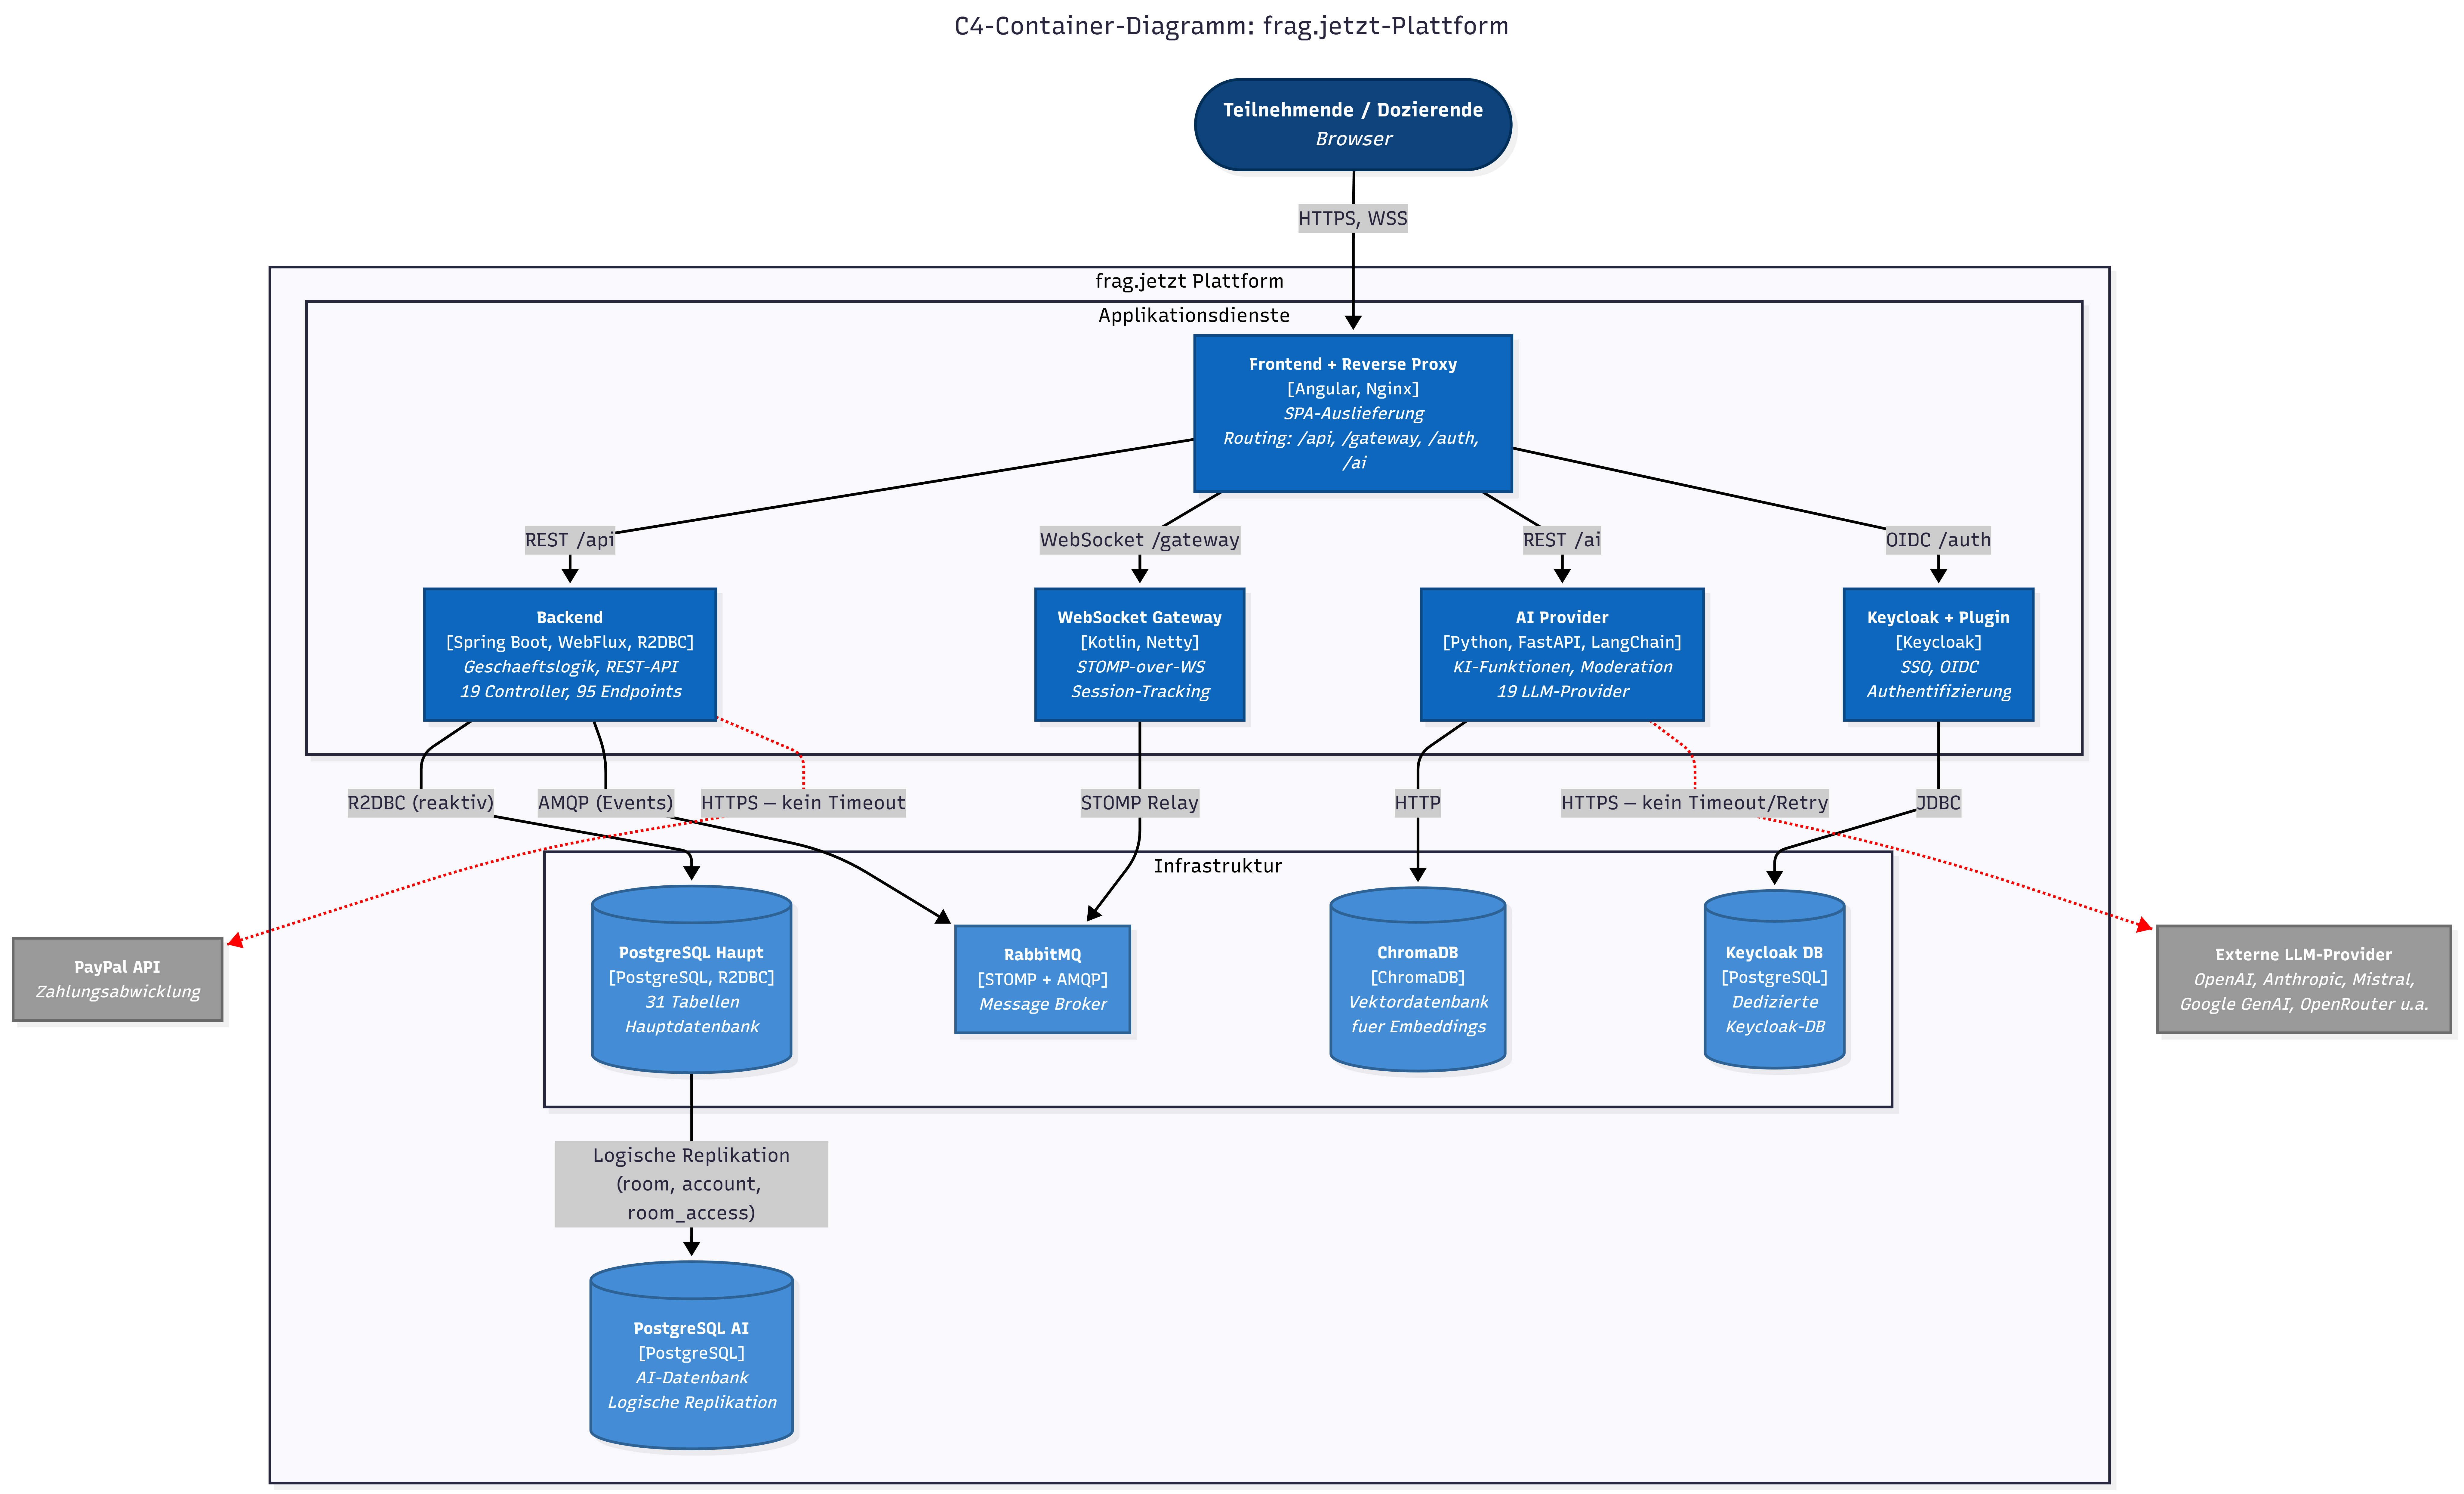
\includegraphics[width=\textwidth]{images/frag.jetzt C4-Container-Diagram.png}
\caption[C4-Container-Diagramm der frag.jetzt-Architektur mit Applikationsdiensten, Infrastrukturkomponenten und Kommunikationswegen (Vollseitenansicht des Diagramms in Anhang~\ref{sec:anhang-c4-vollansicht}).]{C4-Container-Diagramm der frag.jetzt-Architektur mit Applikationsdiensten, Infrastrukturkomponenten und Kommunikationswegen (Vollseitenansicht des Diagramms in Anhang~\ref{sec:anhang-c4-vollansicht}). \small Quelle: Eigene Darstellung.}
\label{fig:c4-fragjetzt-architektur}
\end{figure} 

\section{Kritische User Journeys}

Eine wirksame Observability-Strategie orientiert sich an den tatsächlichen Nutzungspfaden, nicht an abstrakten Systemkomponenten \parencite[S.~10--11]{Niedermaier2019onObservability}. Für frag.jetzt lassen sich drei geschäftskritische Abläufe identifizieren.

\subsection{Journey 1: Frage stellen.}
Die Frage wird vom Frontend per REST an das Backend übermittelt, dort validiert, in der Datenbank persistiert -- wobei ein Trigger eine Kommentarnummer generiert -- und über RabbitMQ als Echtzeit-Update an alle Raum-Clients weitergeleitet. Der Ablauf durchläuft vier Komponenten; Messgrößen sind Backend-Antwortzeit, Dauer des DB-Inserts und WebSocket-Zustelllatenz.

\subsection{Journey 2: Live-Voting.}
Votes werden per REST persistiert. Ein Trigger aktualisiert synchron die Score-Spalte der zugehörigen Frage; bei parallelen Abstimmungen entsteht Row-Level Contention, die unter Spitzenlast zu steigenden Antwortzeiten führen kann (vgl. Abschnitt~3.4, R2).

\subsection{Journey 3: KI-Zusammenfassung.}
Die Anfrage gelangt vom Frontend über das Backend an den AI Provider, der einen externen LLM-Dienst aufruft. Kein externer Aufruf im System hat einen konfigurierten Timeout; ein nicht reagierender Upstream-Dienst kann daher Request-Laufzeiten unbegrenzt verlängern und die rechtzeitige Antwortlieferung an das Frontend gefährden.


\section{Risikopunkte und Zuordnung zu den Golden Signals}

Aus der Architekturanalyse lassen sich sechs Risikopunkte ableiten, die in Tabelle~\ref{tab:risiken} den betroffenen Golden Signals und ihrer Nutzerwirkung zugeordnet werden.

\subsection{R1: Fehlende Timeouts und Resilienz.}
Weder Backend noch AI Provider konfigurieren Timeouts, Retries oder Circuit Breaker auf ausgehenden HTTP-Aufrufen. Ein nicht reagierender externer Dienst kann Request-Laufzeiten unbegrenzt verlängern und die Ressourcenauslastung erhöhen.

\subsection{R2: Datenbankengpässe bei Massenabstimmungen.}
Die Vote-Trigger führen bei jedem Schreibvorgang einen zusätzlichen \texttt{SELECT} und \texttt{UPDATE} auf der Comment-Tabelle aus; bei gleichzeitigen Abstimmungen entsteht Row-Level Contention.

\subsection{R3: Backend als Single Point of Failure ohne Observability.}
Nahezu alle Nutzerinteraktionen laufen über das Backend, das gleichzeitig über keinerlei Observability-Infrastruktur verfügt -- weder Actuator noch Metriken, weder Tracing noch strukturierte Logs. Fehler bleiben unsichtbar, bis Endnutzende Symptome wahrnehmen.

\subsection{R4: WebSocket-Verbindungsverlust.}
Für RabbitMQ existieren keine Health-Checks. Ein Broker-Ausfall unterbricht alle Echtzeit-Updates, bleibt aber ohne Überwachung der Queue-Tiefe und Subscription-Anzahl zunächst unbemerkt.

\subsection{R5: Fehlende Ressourcenlimits.}
Kein Container definiert CPU- oder Speicherlimits. Ein einzelner Dienst mit unkontrolliertem Ressourcenverbrauch kann durch Ressourcenverdrängung alle übrigen Dienste beeinträchtigen.

\subsection{R6: Single-Host-Topologie als systemweiter Ausfallpfad.}
Alle zehn Container laufen auf einem gemeinsamen Host. Ein Hardware- oder Betriebssystemausfall betrifft das Gesamtsystem; in Kombination mit R5 entsteht ein einzelner Sättigungspfad, über den ein Dienst alle übrigen destabilisieren kann.

\begin{table}[ht]
\centering
\caption[Zuordnung der Risikopunkte zu Golden Signals und Nutzerwirkung.]{Zuordnung der Risikopunkte zu Golden Signals und Nutzerwirkung. \small Quelle: Eigene Darstellung.}
\label{tab:risiken}
\small
\begin{tabularx}{\textwidth}{l l l X}
\toprule
\textbf{Risiko} & \textbf{Dienst(e)} & \textbf{Signale} & \textbf{Nutzerwirkung} \\
\midrule
R1 & Backend, AI Provider & Latency, Errors & Hängende Anfragen, Timeouts \\
R2 & Backend, PostgreSQL & Latency, Saturation & Verzögerte Votes in Spitzenlast \\
R3 & Backend & Alle & Fehler erst durch Nutzerbeschwerden sichtbar \\
R4 & WS-Gateway, RabbitMQ & Errors, Traffic & Ausbleibende Echtzeit-Updates \\
R5 & Alle Container & Saturation & Systemweite Instabilität \\
R6 & Gesamtsystem & Saturation, Errors & Totalausfall bei Host-Ausfall \\
\bottomrule
\end{tabularx}
\end{table}


\section{Observability-Ist-Zustand}

Die Quellcode-Analyse ergibt, dass die bestehende Observability-Infrastruktur minimal ist. Das Backend besitzt weder Actuator noch Metriken, kein Tracing und keine strukturierten Logs. Das WS-Gateway konfiguriert einen Health- und Prometheus-Endpunkt, jedoch ist die benötigte Micrometer-Registry nicht als Abhängigkeit deklariert. RabbitMQ hat das Prometheus-Plugin aktiviert, der Port wird aber nicht exponiert. Systemweit fehlen Distributed Tracing, Korrelations-IDs, zentrale Log-Aggregation und ein Monitoring-Stack vollständig. Störungen werden gegenwärtig erst wahrgenommen, wenn Endnutzende direkt betroffen sind -- ein Zustand, den \textcite[S.~9--10]{Niedermaier2019onObservability} als Folge einer rein reaktiven Monitoring-Implementierung einordnen.


\section{Ableitung der Observability-Anforderungen}

Aus Architektur, Kernabläufen, Risikopunkten und Ist-Zustand lassen sich fünf Anforderungen ableiten.

\subsection{A1: Ende-zu-Ende-Nachvollziehbarkeit über Dienstgrenzen.}
Die User Journeys durchlaufen jeweils mehrere Dienste; kausale Zusammenhänge zwischen Störungen sind ohne dienstübergreifende Sichtbarkeit nicht erkennbar. \textcite[S.~6]{albuquerque2025tracing} beschreiben \emph{Distributed Tracing} als grundlegendes Entwurfsmuster für diese Anforderung: Jeder eingehenden Anfrage wird eine eindeutige ID zugewiesen, die über alle Dienste propagiert und in Logs sowie Spans mitgeführt wird, sodass der gesamte Ausführungspfad rekonstruierbar ist.

\subsection{A2: Mehrstufige Messbarkeit entlang der Golden Signals.}
Die Instrumentierung muss auf drei Ebenen erfolgen: (1)~Browser-Telemetrie im Frontend für Nutzererfahrungsmetriken, (2)~Service-Metriken für Latenz, Durchsatz, Fehlerrate und Sättigung der vier Applikationsdienste und der Datenbank, sowie (3)~Infrastruktur-Metriken für Container-Ressourcen, Verbindungspools und Queue-Tiefen. \textcite[S.~10, 16]{albuquerque2025tracing} beschreiben \emph{Application Metrics} und \emph{Infrastructure Metrics} als komplementäre Entwurfsmuster, deren Zusammenspiel erst eine ganzheitliche Systemsicht ermöglicht \parencite[S.~22]{albuquerque2025tracing}.

\subsection{A3: Strukturiertes, korrelierbares Logging.}
Das Logging muss auf strukturierte Formate (JSON) mit Korrelations-IDs umgestellt und zentral aggregiert werden, damit Logeinträge verschiedener Dienste einer gemeinsamen Anfrage zugeordnet werden können \parencite[S.~9--10]{albuquerque2025tracing}.

\subsection{A4: Handlungsfähige Alarmierung.}
Alarme sollen auf nutzerwirksame Zustände reagieren -- steigende Antwortzeiten, wachsende Fehlerraten oder nicht erreichbare Schnittstellen -- und ausreichend Kontext für eine gezielte Erstreaktion enthalten. Formale SLOs existieren derzeit nicht und können als zukünftige Weiterentwicklung betrachtet werden.

\subsection{A5: Beobachtbarkeit der Infrastrukturschicht.}
Die Single-Host-Topologie (R6) und die fehlenden Ressourcenlimits (R5) erzeugen blinde Flecken, die nur durch Infrastruktur-Metriken sichtbar werden. Die Strategie muss Container-Ressourcenverbrauch, Datenbankverbindungspool-Auslastung, RabbitMQ-Queue-Tiefen und Dienstverfügbarkeit über Health-Endpunkte einbeziehen. \textcite[S.~10]{Niedermaier2019onObservability} formulieren eine solche ganzheitliche Sicht über System- und Infrastrukturebenen hinweg als Kernanforderung an Monitoring-Konzepte verteilter Systeme.

\bigskip

Diese Anforderungen bilden die Grundlage der folgenden Kapitel: A1--A3 adressieren primär Forschungsfrage~1, A2 und A5 liefern Evaluationskriterien für Forschungsfrage~2, und A4 bildet die Grundlage für Forschungsfrage~3.
% !TEX root = ../Thesis.tex
 
% =============================================================================
% KAPITEL 4 – Methodisches Vorgehen und Bewertungsrahmen
% =============================================================================

\chapter{Methodisches Vorgehen und Bewertungsrahmen}
 
Dieses Kapitel legt das methodische Vorgehen offen, mit dem aus den theoretischen Grundlagen (Kapitel~2) und der Systemanalyse (Kapitel~3) eine konkrete Observability-Strategie für frag.jetzt entsteht. Es beschreibt zunächst die Arbeitslogik der Arbeit, dann das Verfahren zur servicebezogenen Ableitung der Golden Signals und abschließend die Kriterien für Stack-Auswahl und Evaluation.
 
 
\section{Arbeitslogik der Arbeit}
 
Die Arbeit folgt einer konstruktiv-artefaktorientierten Arbeitslogik. Auf Basis der theoretischen Fundierung und der Systemanalyse werden Observability-Anforderungen abgeleitet. Darauf aufbauend wird eine Observability-Strategie entwickelt, in ausgewählten Komponenten prototypisch umgesetzt und anhand zuvor definierter Kriterien bewertet. Der Schwerpunkt liegt auf der systematischen Entwicklung und Beurteilung eines konkreten Lösungskonzepts für einen realen Anwendungskontext, nicht auf einem empirischen Forschungsdesign im engeren Sinne.
 
Die Arbeitsschritte gliedern sich in fünf aufeinander aufbauende Phasen. Die \emph{theoretische Fundierung} (Kapitel~2) erarbeitet die begrifflichen Grundlagen. Die \emph{Systemanalyse} (Kapitel~3) überführt diese in den Kontext von frag.jetzt und leitet fünf Observability-Anforderungen (A1--A5) ab. Die \emph{Stack-Evaluation} (Kapitel~5) bewertet verfügbare Technologiekombinationen anhand der in Abschnitt~4.3 definierten Vergleichskriterien. Die \emph{Strategiekonzeption mit prototypischer Umsetzung} (Kapitel~6 und~7) bildet den Kern der Eigenleistung: Hier werden die Four Golden Signals dienstspezifisch operationalisiert, eine Telemetrie-Pipeline entworfen sowie Dashboards und Alerting-Regeln konzipiert. Abschließend prüft die \emph{Evaluation} (Kapitel~8) die Strategie gegen die Bewertungskriterien und die Anforderungen aus Kapitel~3.
 
Die Architekturerhebung in Kapitel~3 stützt sich ergänzend auf eine KI-gestützte Quellcodeexploration mithilfe von GitHub Copilot. Das Werkzeug diente als Explorationshilfe, um Architekturübersichten, Controller-Strukturen und bestehende Konfigurationen aus der umfangreichen Codebasis systematisch zu extrahieren. Sämtliche architekturrelevanten Befunde, insbesondere Serviceabhängigkeiten, Datenbankzugriffe, externe Anbindungen und vorhandene Monitoring-Konfigurationen, wurden anschließend durch manuelle Prüfung gegen Quellcode, Docker-Compose-Dateien und Konfigurationsartefakte validiert. GitHub Copilot fungierte dabei ausschließlich als unterstützendes Analysewerkzeug, nicht als eigenständiger Erkenntnisträger. Das Verfahren erfasst implizite Laufzeitabhängigkeiten und Konfigurationen außerhalb des versionierten Quellcodes nur eingeschränkt. Diese Grenzen werden bei der Anforderungsableitung berücksichtigt.
 
 
\section{Vorgehen bei der Ableitung der Golden Signals pro Service}
 
Die Four Golden Signals (Latency, Traffic, Errors und Saturation) bilden den heuristischen Rahmen für die servicebezogene Instrumentierung \parencite[Kap.~\emph{The Four Golden Signals}]{ewaschukMonitoringDistributedSystems}. Die Herausforderung liegt weniger in der Kenntnis der vier Kategorien als in ihrer konkreten Übersetzung auf heterogene Dienste mit unterschiedlichen Rollen und Kommunikationsmustern. Damit diese Übersetzung nachvollziehbar erfolgt, folgt die Arbeit einer fünfstufigen Ableitungslogik.
 
Im ersten Schritt wird die \emph{Rolle des Dienstes im Gesamtsystem} bestimmt. Die funktionale Einordnung -- ob Einstiegspunkt für Nutzerinteraktionen, zentrale Geschäftslogik, Datenhaltung oder Anbindung externer Ressourcen -- beeinflusst maßgeblich, welche Beobachtungsgrößen aussagekräftig sind.
 
Der zweite Schritt identifiziert die \emph{kritischen Interaktionen} des Dienstes. Hierzu dienen die User Journeys und Risikopunkte aus Kapitel~3 als Eingangsgröße. Metriken sollten an realen Nutzungspfaden ausgerichtet sein, nicht an abstrakten Komponentengrenzen \parencite[S.~10--11]{Niedermaier2019onObservability}.
 
Auf dieser Grundlage werden im dritten Schritt \emph{geeignete Messgrößen} abgeleitet. Wo fachlich sinnvoll, wird pro Golden Signal mindestens eine primäre Messgröße bestimmt. Ergänzend können Logs, Traces oder Black-Box-Indikatoren herangezogen werden. Nicht jedes Signal lässt sich bei jedem Dienst gleichermaßen als White-Box-Metrik erfassen. Bei externen KI-Services etwa ist Saturation nur indirekt über Antwortzeiten und Timeout-Raten beobachtbar. \textcite[Kap.~\emph{Symptoms Versus Causes}]{ewaschukMonitoringDistributedSystems} betont die Unterscheidung zwischen symptomorientierten und ursachenorientierten Beobachtungsgrößen. Für die Alarmierung sind Symptome entscheidend, während Ursachenindikatoren primär als Debugging-Kontext dienen. \textcite[S.~10, 16]{albuquerque2025tracing} differenzieren zudem zwischen \emph{Application Metrics} und \emph{Infrastructure Metrics} als komplementären Entwurfsmustern, deren Zusammenspiel erst eine vollständige Sicht auf das Verhalten eines Dienstes ermöglicht \parencite[S.~22]{albuquerque2025tracing}.
 
Der vierte Schritt begründet \emph{initiale Ziel- und Schwellenwerte}. Da für frag.jetzt keine historischen Produktivdaten vorliegen, werden zunächst operative Startschwellen auf Basis von Lasttests und Erfahrungswerten festgelegt. Diese dienen als Ausgangspunkt für begründete Zielwerte, die zunächst in einer Staging-Umgebung anhand definierter Last- und Störungsszenarien überprüft und bei Bedarf angepasst werden. Formale Service Level Objectives, wie sie im SRE-Kontext als quantifizierbare Zielvorgaben die Instrumentierung und Alarmierung strukturieren \parencite[S.~605]{hallur2024monitoring}, existieren für frag.jetzt derzeit nicht und werden als zukünftige Weiterentwicklung betrachtet. \textcite[S.~9]{Niedermaier2019onObservability} bestätigen, dass unklare nichtfunktionale Anforderungen und eine reaktive Monitoring-Entwicklung zu den häufigsten Herausforderungen verteilter Systeme gehören. Ein Ausgangszustand, der auch auf frag.jetzt zutrifft.
 
Im fünften Schritt wird bestimmt, welche \emph{Visualisierung und Alarmierung} aus den Messgrößen folgen. Nicht jede Metrik rechtfertigt einen eigenen Alarm. Alarme sollten auf nutzerseitig wahrnehmbare Symptome ausgerichtet sein, während interne Ursachenindikatoren als Debugging-Kontext bereitstehen \parencite[S.~175]{vinnakota2025creating}. Ebenso bestimmt die Zielgruppe die Aufbereitung. Eine p99-Latenzverteilung eignet sich für ein DevOps-Dashboard, während ein Product Owner eher aggregierte Verfügbarkeitsindikatoren benötigt.
 
Diese Logik stellt sicher, dass die Signal-Ableitung in Kapitel~6 nachvollziehbar an die Systemanalyse rückgebunden bleibt.
 
 
\section{Kriterien für Stack-Auswahl und spätere Evaluation}
 
Die Arbeit verwendet zwei aufeinander abgestimmte, aber bewusst getrennte Kriterienebenen. Die Stack-Auswahl (Kapitel~5) beantwortet die Werkzeugfrage, welche Technologiekombination die Anforderungen am besten adressiert. Die Evaluation (Kapitel~8) beantwortet die Ergebnisfrage, ob die entwickelte Strategie tatsächlich die identifizierten Probleme löst.
 
\subsection{Vergleichskriterien für die Stack-Auswahl}
 
Eine systematische Stack-Auswahl erfordert mehr als bloße Feature-Listen. Bei der Wahl von Observability-Werkzeugen müssen Faktoren wie Datenaufnahmeraten, Abfrageleistung, Speicherkosten und Integrationsfähigkeit berücksichtigt werden \parencite[S.~104]{sakinala2025observability}. \textcite[S.~72015]{faseeha2025observability} schlagen eine thematische Taxonomie vor, die Werkzeuge nach Einsatzzweck, erfassten Parametern und Architekturmustern vergleichbar macht. \textcite[S.~3]{giamattei2024monitoring} operationalisieren einen ähnlichen Ansatz, indem sie funktionale und technologische Merkmale systematisch gegenüberstellen.
 
Aufbauend auf diesen Vorarbeiten und den Anforderungen A1--A5 werden folgende Vergleichskriterien verwendet:
 
\begin{itemize}
    \item \textbf{Abdeckung der Telemetriepfeiler.} Unterstützung von Metriken, Logs und Traces in integrierter Form.
    \item \textbf{Korrelationsfähigkeit.} Verknüpfung verschiedener Telemetriearten über gemeinsame Bezeichner (Trace-IDs, Korrelations-IDs).
    \item \textbf{OpenTelemetry-Kompatibilität.} Unterstützung des herstellerneutralen CNCF-Standards für Instrumentierung und Datenexport, um Vendor Lock-in zu vermeiden.
    \item \textbf{Dashboarding und Alerting.} Eignung des Stacks für die Erstellung rollenspezifischer Dashboards sowie für die Definition und Verwaltung differenzierter Alarmregeln.
    \item \textbf{Integrationsaufwand.} Technischer Aufwand für die Einbindung in die bestehende Docker-Compose-Topologie und die vorhandenen Technologien (Spring Boot, Kotlin/Netty, Python/FastAPI).
    \item \textbf{Ressourcenbedarf.} Zusätzlicher Speicher-, CPU- und Festplattenbedarf auf einem einzelnen Host, besonders relevant angesichts der Single-Host-Topologie von frag.jetzt (vgl.~R6).
    \item \textbf{Erweiterbarkeit.} Anpassungsfähigkeit bei steigenden Anforderungen, etwa wachsendem Telemetrievolumen oder zusätzlichen Diensten.
    \item \textbf{Community und Ökosystem.} Breite der Nutzerbasis, Dokumentationsreife und Integrationen mit gängigen Frameworks.
\end{itemize}
 
Die Gesamtbewertung eines Stacks wird abschließend unter dem Gesichtspunkt der \emph{Eignung für frag.jetzt} zusammengeführt. Dabei fließen die Einzelkriterien gewichtet in eine Synthese ein, die den spezifischen Kontext (Single-Host-Betrieb, begrenztes Betriebsteam, heterogene Technologielandschaft) explizit berücksichtigt.
 
\subsection{Bewertungskriterien für die Gesamtstrategie}
 
Die Gesamtstrategie wird an einem übergeordneten Maßstab gemessen, der direkt auf die Anforderungen A1--A5 aus Kapitel~3 zurückgreift. \textcite[S.~9--10]{Niedermaier2019onObservability} formulieren eine ganzheitliche Sicht über System- und Infrastrukturebenen hinweg als Kernanforderung an Monitoring-Konzepte verteilter Systeme. Diese Perspektive wird hier aufgegriffen und in prüfbare Evaluationsfragen überführt.
 
Für jede Anforderung wird eine konkrete Prüffrage formuliert: Lässt sich ein Request Ende-zu-Ende rekonstruieren (A1)? Deckt die Instrumentierung alle drei Messebenen ab (A2)? Können Logeinträge über Korrelations-IDs verknüpft werden (A3)? Reagieren Alarme auf nutzerwirksame Zustände und enthalten sie ausreichend Kontext für eine Erstreaktion (A4)? Werden Container-Ressourcen, Datenbankpool-Auslastung und Queue-Tiefen erfasst (A5)? Für die Alarmierungsqualität betonen \textcite[S.~3]{gowda2022alerts}, dass ein Alarm nur dann operativen Wert besitzt, wenn er Problem, Schweregrad, betroffene Komponenten und empfohlene Gegenmaßnahmen klar benennt.
 
Die Beantwortung dieser Fragen stützt sich auf drei Evidenzquellen: erstens die \emph{Artefaktanalyse}, bei der Instrumentierungskonfigurationen, Dashboard-Definitionen und Alarmregeln gegen die Anforderungen geprüft werden. Zweitens die \emph{Konfigurations- und Instrumentierungsprüfung}, die sicherstellt, dass die definierten Metriken, Logs und Traces tatsächlich erhoben und korrekt korreliert werden. Drittens ausgewählte \emph{Last- und Störungsszenarien}, die in einer produktionsnahen Testumgebung gezielt Lastspitzen und Fehlerbilder simulieren.
 
Ergänzend fließen drei übergreifende Bewertungsdimensionen ein: die \emph{Stakeholder-Tauglichkeit}, also ob Dashboards den unterschiedlichen Rollen die jeweils benötigten Informationen liefern, die \emph{Abdeckung der Risikopunkte} R1--R6 aus Kapitel~3 und der \emph{Umsetzungsrealismus}, also ob die Strategie mit den verfügbaren Mitteln und der bestehenden Infrastruktur implementierbar ist.
 
Die Evaluation in Kapitel~8 gleicht diese Kriterien mit den Ergebnissen der prototypischen Umsetzung ab. Zu diesem Zweck werden in einer produktionsnahen Staging-Umgebung gezielt Lastspitzen und Fehlerszenarien erzeugt, um die Instrumentierung, Korrelation und Alarmierungslogik kontrolliert zu prüfen. Die Aussagekraft dieser Validierung bleibt gegenüber Beobachtungen aus einem langfristigen Produktivbetrieb begrenzt und wird in Kapitel~8 entsprechend eingeordnet.



% \newpage

% \chapter{Implementierung und Ergebnisse}
% \index{Implementierung}%
% \index{Benchmark}%
% \index{Evaluation}%
% \label{ch:realisierung}

% \section{Implementierungsdetails}

% Das Kapitel dokumentiert die praktischen Aspekte der Umsetzung\index{Implementierungspraxis}.\footnote{Implementierungsdetails orientieren sich an Best Practices aus~\cite{martin2008clean}.}
% Die Implementierung erfolgte iterativ\index{Iterative Entwicklung} über einen Zeitraum von 4 Monaten mit kontinuierlichem Testen\index{Continuous Testing} und Verfeinerung.

% \subsection{Technologiestack}

% Folgende Technologien wurden für die Implementierung eingesetzt:

% \begin{sloppypar}
% \begin{description}
%   \item[Programmiersprache:] Python 3.11+\index{Python} (Typ-Hinweise\index{Type Hints}, Async/Await-Un\-ter\-stüt\-zung\index{Async/Await})
%   \item[LLM-Integration:] OpenAI API (GPT-4)\index{GPT-4}, Anthropic API (Claude 3.5 Sonnet)\index{Claude}, mit Fallback-Mechanismus\index{Fallback-Mechanismus}
%   \item[Orchestrierung:] LangChain 0.1.x für Basis-Komponenten\index{LangChain}, benutzerdefinierte Erweiterungen für SE-spezifische Tools; strukturierte Tool-Calls über \textbf{JSON}-Schemas und Konfigurationen per \textbf{YAML}.
%   \item[Gedächtnis:] Chroma\index{Chroma Vector-DB} Vektordatenbank für semantisches Retrieval, SQLite für episodische Logs\index{Event-Logging}
%   \item[Werkzeuglaufzeitumgebung:] Docker 24.0+\index{Docker!Sandboxing} für Sandboxing, pytest für Tests, ruff/black für Linting\index{Code Linting}
%   \item[Monitoring:] Prometheus für Metriken\index{Prometheus}, strukturierte Logs (JSON) mit Trace-IDs\index{Distributed Tracing}
% \end{description}
% \end{sloppypar}

% \subsection{Projektstruktur}

% Das Projekt folgt einer modularen Architektur:

% \begin{lstlisting}[breaklines=true, basicstyle=\ttfamily\small]
% agent_se/
% +-- core/
% |   +-- agent.py           # Agent Controller (ReAct-Loop)
% |   +-- policy.py          # Planning & Reflection Logic
% |   +-- state.py           # State Management
% +-- tools/
% |   +-- base.py            # Tool Interface & Registry
% |   +-- code_tools.py      # Linter, Formatter, AST-Parser
% |   +-- test_tools.py      # pytest, coverage, Test-Runner
% |   +-- vcs_tools.py       # git operations
% +-- memory/
% |   +-- episodic.py        # Event Logging & Retrieval
% |   +-- semantic.py        # Vector Store Integration
% +-- safety/
% |   +-- validator.py       # Input Validation & Sanitization
% |   +-- sandbox.py         # Docker-based Execution Env
% +-- evaluation/
%     +-- benchmarks.py      # Test Scenarios
%     +-- metrics.py         # Success Rate, Costs, Latency
% \end{lstlisting}

% \subsection{Kernimplementierung: Agent-Controller}\index{Agent Controller!Implementierung}

% Listing \ref{lst:agent-loop} zeigt eine minimale agentische Schleife\index{Agent Loop} mit Planung\index{Planung!Implementierung}, Werkzeugausführung und Reflexion\index{Reflexion}. Die vollständige Implementierung umfasst zusätzlich Fehlerbehandlung\index{Error-Handling!Agent}, Timeouts, Schrittbegrenzungen und strukturiertes Logging\index{Agent Logging}.

% \begin{lstlisting}[style=Python, caption={Minimaler agentischer Loop für SE-Aufgaben (Beispiel-Listing)}, label={lst:agent-loop}]
% from typing import Dict, Any

% class Toolset:
%   def run_tests(self) -> str:
%     return "tests: 103 passed, 2 failed"

%   def format_code(self, diff: str) -> str:
%     return "formatted diff applied"

% class Agent:
%   def __init__(self, tools: Toolset):
%     self.tools = tools
%     self.memory = []  # episodic traces

%   def plan(self, goal: str) -> str:
%     return f"Plan: run tests -> fix failures -> re-run -> format -> commit ({goal})"

%   def act(self, step: str) -> str:
%     if "run tests" in step:
%       return self.tools.run_tests()
%     if "format" in step:
%       return self.tools.format_code(diff="...")
%     return "noop"

%   def reflect(self, observation: str) -> str:
%     if "failed" in observation:
%       return "Next: inspect failing tests and patch code"
%     return "Next: finalize and commit"

%   def run(self, goal: str) -> Dict[str, Any]:
%     plan = self.plan(goal)
%     self.memory.append({"plan": plan})
%     obs = self.act("run tests")
%     self.memory.append({"obs": obs})
%     next_step = self.reflect(obs)
%     self.memory.append({"reflect": next_step})
%     obs2 = self.act("format")
%     self.memory.append({"obs": obs2})
%     return {"status": "done", "trace": self.memory}

% agent = Agent(Toolset())
% result = agent.run(goal="increase reliability of module X")
% print(result["status"])
% \end{lstlisting}

% Listing~\ref{lst:ts-tool-calling} zeigt ergänzend die Implementierung eines Tool-Aufrufs in TypeScript.

% % ------------------------------------------------------------
% % Zweites Listing: TypeScript Tool-Calling Stub
% \begin{lstlisting}[style=TypeScript, caption={Werkzeugaufruf-Stub in TypeScript mit einfachem Funktionsschema (Beispiel-Listing)}, label={lst:ts-tool-calling}]
% type ToolName = "run_tests" | "format_code" | "open_issue";

% interface ToolCall {
%   name: ToolName;
%   args: Record<string, unknown>;
% }

% interface ToolResult {
%   name: ToolName;
%   ok: boolean;
%   output: string;
% }

% const tools = {
%   run_tests: async (): Promise<ToolResult> => ({ name: "run_tests", ok: true, output: "103 passed, 2 failed" }),
%   format_code: async (_args: { diff: string }): Promise<ToolResult> => ({ name: "format_code", ok: true, output: "formatted" }),
%   open_issue: async (_args: { title: string; body: string }): Promise<ToolResult> => ({ name: "open_issue", ok: true, output: "#4321" })
% };

% async function dispatch(call: ToolCall): Promise<ToolResult> {
%   switch (call.name) {
%     case "run_tests":
%       return tools.run_tests();
%     case "format_code":
%       return tools.format_code(call.args as { diff: string });
%     case "open_issue":
%       return tools.open_issue(call.args as { title: string; body: string });
%   }
% }

% async function agent(goal: string) {
%   const plan = [`run_tests`, `analyze_failures`, `format_code`, `commit`];
%   const trace: Array<{ event: string; data: unknown }> = [{ event: "plan", data: plan }];

%   const res1 = await dispatch({ name: "run_tests", args: {} });
%   trace.push({ event: "tool_result", data: res1 });

%   if (res1.output.includes("failed")) {
%     // Simple reflection -> open an issue with details
%     const res2 = await dispatch({ name: "open_issue", args: { title: `Test failures for ${goal}`, body: res1.output } });
%     trace.push({ event: "tool_result", data: res2 });
%   }

%   const res3 = await dispatch({ name: "format_code", args: { diff: "..." } });
%   trace.push({ event: "tool_result", data: res3 });
%   return { status: "done", trace };
% }

% agent("increase reliability of module X").then(r => console.log(r.status));
% \end{lstlisting}

% \section{Experimentelles Setup}

% Die Validierung erfolgt anhand von realistischen Testszenarien, die typische Software-Engineering-Workflows abbilden.

% \subsection{Testumgebung}

% \begin{sloppypar}
% \begin{description}
%   \item[Hardware:] MacBook Pro M2, 16\,GB RAM, 512\,GB SSD
%   \item[Betriebssystem:] macOS 14.x, Docker Desktop 4.25
%   \item[LLM-Modelle:] GPT-4-Turbo (0125), Claude 3.5 Sonnet, mit Temperatur 0.2 für Reproduzierbarkeit
%   \item[Testdaten:] 25 repräsentative Python-Projekte (5\,k--50\,k LOC), synthetische Bugs, real-world Issues
% \end{description}
% \end{sloppypar}

% \subsection{Benchmark-Szenarien}

% Drei Haupt-Szenarien wurden evaluiert (vgl. Kapitel~\ref{ch:konzept}):

% \begin{enumerate}
%   \item \textbf{Automated Refactoring} (10 Tasks): Extract-Function, Rename-Variable, Simplify-Conditional
%   \item \textbf{Test Failure Diagnosis} (8 Tasks): Debug failing tests, fix assertions, update mocks
%   \item \textbf{Lint Error Resolution} (7 Tasks): Fix style issues, type errors, unused imports
% \end{enumerate}

% Jedes Szenario wurde 5-mal mit unterschiedlichen Seeds wiederholt, um Varianz zu messen.

% \subsection{Beispiel: Test Failure Diagnosis — Schritt-für-Schritt}

% Im Folgenden wird das Szenario \enquote{Test Failure Diagnosis} detailliert beschrieben, um den praktischen Ablauf und die typischen Artefakte (Tool-Calls, Logs, Entscheidungen) zu veranschaulichen.

% 1) Initialer Zustand: Test-Runner meldet \texttt{3 failed} in \texttt{auth/test\_login.py}. Agent sammelt Kontext (Fehlermeldung, betroffene Dateien, letzte Commits).

% 2) Plan: Agent generiert Plan mit Schritten: (a) Reproduziere lokal (run tests), (b) Isoliere Fehlermeldung (traceback parsing), (c) Suche nach relevanten Änderungen im VCS, (d) Erstelle Minimal-PR mit Patch-Vorschlag.

% 3) Act: Tool-Calls (Beispiel):
% \begin{itemize}
%   \item \texttt{run\_tests(module="auth")} \textrightarrow\ \texttt{"3 failed, 97 passed"}
%   \item \texttt{run\_linter(path="auth/")} \textrightarrow\ Tool-Result: Hinweise auf Stil, aber keine direkten Fehler
%   \item \texttt{search\_in\_repo(query="login", range="last-5-commits")} \textrightarrow\ Treffer: Commit 123abc \texttt{Refactor: auth flow}
% \end{itemize}

% 4) Observation: Agent parst Traceback, findet NullPointer-ähnlichen Fehler in Hilfsfunktion, die neu extrahiert wurde. Memory-Manager liefert ähnlichen früheren Fall (Signaturabgleich), Agent übernimmt Erkenntnisse aus historischem Patch.

% 5) Reflection 
% \begin{sloppypar}
% \begin{itemize}
%   \item Agent generiert Patch-Vorschlag (kleine Scope-Korrektur im Helper), erstellt Diff und führt Tests erneut in isolierter Sandbox aus.
%   \item Tests grün $\Rightarrow$ Agent eröffnet PR-Entwurf und notiert Review-Kommentare; bei Teil-Erfolg: Human-Approval-Gate vor Merge.
% \end{itemize}
% \end{sloppypar}

% Beispiel-Trace (gekürzt):
% \begin{lstlisting}[breaklines=true, basicstyle=\ttfamily\small]
% [Agent] run_tests -> 3 failed (auth/test_login.py::test_login)
% [Agent] search_in_repo -> found commit 123abc (Refactor auth flow)
% [Agent] generate_patch -> diff created: modify auth/helpers.py
% [Agent] run_tests (sandbox) -> 100 passed
% [Agent] open_pr -> PR #42 (Draft)
% \end{lstlisting}

% Das Beispiel zeigt, wie Tool-Adapter, Memory und Safety-Layer (Sandbox, Human-Approval) zusammenwirken, um fehlerhafte Änderungen sicher zu erkennen und zu beheben. Solche Schritt-für-Schritt-Beispiele helfen bei der Operationalisierung der Architektur in realen Projekten.

% \section{Ergebnisse}

% Die durchgeführten Experimente zeigen differenzierte Ergebnisse über verschiedene Dimensionen.

% \subsection{Erfolgsraten nach Aufgabentyp}

% Tabelle \ref{tab:benchmark-results} zeigt detaillierte Ergebnisse für ausgewählte Tasks:

% \begin{sloppypar}
% \begin{itemize}
%   \item \textbf{Refactoring:} \pct{73} Erfolgsrate (11/15 Tasks erfolgreich)
%   \item \textbf{Test-Fixing:} \pct{62} Erfolgsrate (5/8 Tasks erfolgreich)
%   \item \textbf{Lint-Resolution:} \pct{86} Erfolgsrate (6/7 Tasks erfolgreich)
% \end{itemize}
% \end{sloppypar}

% Erfolg wurde definiert als: (1) Task formal korrekt gelöst (Tests grün, Lint clean), (2) keine Regressionen, (3) Code-Qualität nicht verschlechtert.

% \subsection{Effizienzmetriken}

% Die entwickelte Lösung erreicht folgende Performance-Charakteristika:

% \begin{sloppypar}
% \begin{description}
%   \item[Token-Verbrauch:] Durchschnittlich 8.4\,k Tokens pro erfolgreichem Task (Range: 2\,k--25\,k). Kontextoptimierung reduzierte Verbrauch um \pct{40} gegenüber naivem Ansatz.
  
%   \item[Laufzeit:] Median 12.3\,Sekunden pro Task (ohne Tool-Execution). Mit Test-Runs: 45\,s--180\,s je nach Testsuite-Größe.
  
%   \item[Tool-Calls:] Durchschnittlich 4.2\,Werkzeugaufrufe pro Task. Reflexion reduzierte fehlerhafte Aufrufe um \pct{28}.
  
%   \item[Kosten:] Geschätzt \$\,0.08 pro Task bei GPT-4-Pricing (Jan 2024). Claude war \pct{35} günstiger bei vergleichbarer Qualität.
% \end{description}
% \end{sloppypar}

% \subsection{Qualitätsmetriken}

% \textquote[\cite{yang2024sweagent}]{Die praktische Implementierung agentischer Systeme erfordert sorgfältige Planung und umfassende Tests, um Zuverlässigkeit in produktiven Umgebungen zu gewährleisten.}

% Code-Qualität wurde über mehrere Dimensionen gemessen:

% \begin{sloppypar}
% \begin{itemize}
%   \item \textbf{Test-Pass-Rate:} \pct{98} (nur 2 von 103 Tests regressierten nach Agent-Edits)
%   \item \textbf{Lint-Score:} Durchschnittlich +12 Punkte Verbesserung nach Lint-Fixes
%   \item \textbf{Complexity:} Cyclomatic Complexity blieb unverändert oder verbesserte sich (Extract-Function Tasks)
%   \item \textbf{Review-Akzeptanz:} Manuelles Review ergab \pct{81} Akzeptanzrate („would merge“)
%   \item \textbf{Review-Akzeptanz:} Manuelles Review ergab \pct{81} Akzeptanzrate (\enquote{would merge})
% \end{itemize}
% \end{sloppypar}

% \subsection{Robustheit und Fehlerbehandlung}

% Error-Cases wurden systematisch getestet:

% \begin{sloppypar}
% \begin{itemize}
%   \item \textbf{Werkzeugfehler:} Agent erholte sich in \pct{67} der Fälle durch Wiederholung oder Alternativstrategie
%   \item \textbf{Malformed Outputs:} JSON-Parsing-Fehler wurden durch Wiederholungen mit Schema-Validierung in \pct{89} behoben
%   \item \textbf{Timeouts:} Graceful Degradation bei max-steps Limit (definiert als \pct{15} Partial-Success)
% \end{itemize}
% \end{sloppypar}

% \section{Vergleich mit existierenden Ansätzen}

% Die entwickelte Lösung wurde mit Baselines verglichen:

% \begin{table}[ht]
% \centering
% \caption{Vergleich mit Baseline-Systemen (auf gleichem Benchmark-Set)}
% \label{tab:comparison}
% \begin{tabularx}{\textwidth}{Xcccc}
% \toprule
% \cellcolor{headercolor}\textcolor{white}{\textbf{Ansatz}} & \cellcolor{headercolor}\textcolor{white}{\textbf{Success}} & \cellcolor{headercolor}\textcolor{white}{\textbf{Token}} & \cellcolor{headercolor}\textcolor{white}{\textbf{Zeit (s)}} & \cellcolor{headercolor}\textcolor{white}{\textbf{Kosten}} \\
% \midrule
% Naive Prompting & \pct{42} & 12.3\,k & 8.5 & \$\,0.12 \\
% \rowcolor{rowcolorgray}
% ReAct (Baseline) & \pct{58} & 10.1\,k & 15.2 & \$\,0.10 \\
% Unsere Architektur & \pct{73} & 8.4\,k & 12.3 & \$\,0.08 \\
% \rowcolor{rowcolorgray}
% + Reflexion & \pct{73} & 8.9\,k & 14.1 & \$\,0.09 \\
% \bottomrule
% \end{tabularx}
% \end{table}

% Kernverbesserungen gegenüber Baselines:

% \begin{sloppypar}
% \begin{itemize}
%   \item \textbf{+31\% Erfolgsrate} vs. Naives Prompting durch strukturierte Werkzeugorchestrierung
%   \item \textbf{+15\% Erfolgsrate} vs. Standard-ReAct durch optimiertes Kontextmanagement
%   \item \textbf{-17\% Token-Kosten} durch intelligentes Pruning und Zusammenfassung
%   \item \textbf{Robustere Fehlerbehebung} durch Reflexions-Mechanismen
% \end{itemize}
% \end{sloppypar}

% Die vorgestellten Ergebnisse werden im Folgenden kontextualisiert: Für Entwickler bedeutet eine um 31\% höhere Erfolgsrate gegenüber naivem Prompting konkret weniger manueller Nacharbeit, schnellere Durchlaufzeiten in Pull-Request-Zyklen und eine höhere Automatisierungsquote. Für Betreiber von CI/CD-Infrastrukturen bedeuten niedrigere Token-Kosten und reduzierte Fehlerraten geringere Betriebskosten. Die praktische Perspektive ist wichtig, um Entscheidungsträgern in Unternehmen handfeste Argumente für den Einsatz agentischer Lösungen zu liefern.

% \section{Validierung und Verifikation}

% Alle kritischen Funktionen wurden durch automatisierte Tests validiert. Die Testabdeckung beträgt \pct{87} (Zeilen-Coverage).

% \subsection{Unit-Tests}

% \begin{sloppypar}
% \begin{itemize}
%   \item Tool-Adapter: 45 Tests, \pct{95} Abdeckung
%   \item Policy-Logic: 32 Tests, \pct{89} Abdeckung
%   \item Sicherheitsschicht: 28 Tests, \pct{92} Abdeckung
% \end{itemize}
% \end{sloppypar}

% \subsection{Integrationstests}

% End-to-End-Tests für alle 3 Benchmark-Szenarien. Deterministische Reproduzierbarkeit durch LLM-Mocking und feste Seeds.

% Praktische Erkenntnisse: Automatisierte Tests sollten sowohl synthetische als auch realistische Repositories umfassen; Mocking allein reicht nicht aus, da Tests in realen Umgebungen unerwartete Randfälle aufdecken. Darüber hinaus ist kontinuierliche Überwachung unabdingbar, um Drift in LLM-Verhalten oder Änderungen in abhängigen Tools frühzeitig zu erkennen.

% \subsection{Sicherheits-Audits}

% \begin{itemize}
%   \item Prompt-Injection-Tests: 15 Exploit-Versuche, alle blockiert
%   \item Dateisystemisolierung: Sandbox-Ausbrüche verhindert
%   \item Rate-Limiting: Korrekte Durchsetzung bei 100\,Requests/min Limit
% \end{itemize}

% % Benchmark-Ergebnisse mit longtable
% \begin{table}[ht]
% \centering
% \caption{Detaillierte Benchmark-Ergebnisse: Agentische SE-Tasks mit Evaluationsmetriken}
% \label{tab:benchmark-results}
% \begin{tabularx}{\textwidth}{Xccccc}
% \toprule
% \cellcolor{headercolor}\textcolor{white}{\textbf{Aufgabe}} & \cellcolor{headercolor}\textcolor{white}{\textbf{Success}} & \cellcolor{headercolor}\textcolor{white}{\textbf{Token}} & \cellcolor{headercolor}\textcolor{white}{\textbf{Zeit (s)}} & \cellcolor{headercolor}\textcolor{white}{\textbf{Tools}} & \cellcolor{headercolor}\textcolor{white}{\textbf{Kosten}} \\
% \midrule
% Extract Function & OK & 7.2\,k & 18.5 & 4 & \$\,0.07 \\
% \rowcolor{rowcolorgray}
% Fix Lint Errors & OK & 3.1\,k & 8.2 & 3 & \$\,0.03 \\
% Debug Test Failure & OK & 12.5\,k & 45.3 & 6 & \$\,0.12 \\
% \rowcolor{rowcolorgray}
% Format Code & OK & 2.8\,k & 5.1 & 2 & \$\,0.03 \\
% Rename Variable & OK & 5.4\,k & 12.8 & 3 & \$\,0.05 \\
% \rowcolor{rowcolorgray}
% Remove Deadcode & OK & 8.9\,k & 22.1 & 5 & \$\,0.09 \\
% Update Mocks & FAIL & 9.7\,k & 38.2 & 7 & \$\,0.10 \\
% \rowcolor{rowcolorgray}
% Simplify Conditional & OK & 6.3\,k & 15.7 & 4 & \$\,0.06 \\
% Generate Docstrings & OK & 4.5\,k & 9.3 & 2 & \$\,0.04 \\
% \rowcolor{rowcolorgray}
% Fix Type Errors & OK & 11.2\,k & 28.4 & 5 & \$\,0.11 \\
% \bottomrule
% \multicolumn{6}{l}{\small \textit{Durchschnitt (erfolgreiche Tasks):} 7.1\,k Tokens, 16.5\,s, 3.8\,Tools, \$\,0.07} \\
% \end{tabularx}
% \end{table}

% Tabelle~\ref{tab:eval-metrics} fasst die verwendeten Evaluationsmetriken zusammen.

% % Zusätzliche Beispiel-Tabelle für Evaluationsmetriken
% \begin{table}[ht]
% \centering
% \caption{Evaluationsmetriken für agentische SE-Workflows (Beispieltabelle)}
% \label{tab:eval-metrics}
% \begin{tabularx}{\textwidth}{lX}
% \toprule
% \cellcolor{headercolor}\textcolor{white}{\textbf{Kategorie}} & \cellcolor{headercolor}\textcolor{white}{\textbf{Metriken / Beschreibung}} \\
% \midrule
% Qualität & Task-Success-Rate, Patch-Korrektheit (Tests/Lint), Review-Akzeptanz, Regressionen (\#) \\
% \rowcolor{rowcolorgray}
% Kosten & Token-/API-Kosten (EUR), Werkzeugaufrufkosten, Rechenzeit \\
% Latenz & End-to-End-Laufzeit (s), Tool-Roundtrips (\#), Wartezeit auf CI \\
% \rowcolor{rowcolorgray}
% Sicherheit & Policy-Verstöße (\#), Risk Flags, sand-boxed I/O, PII-Leaks (\#) \\
% Nachvollziehbarkeit & Trace-Länge (\#Events), Artefakte (Patches, Logs), Reproduzierbarkeit (Seeds) \\
% \bottomrule
% \end{tabularx}
% \end{table}

% =============================================================================
% KAPITEL 5 – Evaluation und Auswahl des Observability-Stacks
% =============================================================================


\chapter{Evaluation und Auswahl des Observability-Stacks}
 
\section{Festlegung der Vergleichskriterien}
 
Die acht Vergleichskriterien für die Stack-Auswahl wurden in Abschnitt~4.3 aus den Anforderungen A1--A5 und der einschlägigen Literatur hergeleitet. Sie umfassen die Abdeckung der drei Telemetriepfeiler, Korrelationsfähigkeit, OpenTelemetry-Kompatibilität, Dashboarding und Alerting, Integrationsaufwand, Ressourcenbedarf, Erweiterbarkeit sowie Community und Ökosystem. Im Kern adressieren die Anforderungen drei Kernbedürfnisse, nämlich eine durchgängige Nachvollziehbarkeit dienstübergreifender Abläufe (A1), eine mehrstufige Messbarkeit vom Infrastruktur- bis zum Anwendungsniveau (A2) sowie ein korrelierbares, strukturiertes Logging (A3). Hinzu kommen die Betriebsrestriktionen einer Single-Host-Topologie (A4) und das Erfordernis, alle Stakeholder-Rollen mit handlungsorientierten Informationen zu versorgen (A5). Das vorliegende Kapitel wendet diese Kriterien auf drei vollständige Observability-Architekturen an, um Forschungsfrage~2 zu beantworten: Welche Observability-Stack-Kombination eignet sich am besten für die Überwachungsanforderungen von frag.jetzt?
 
 
\section{OpenTelemetry als verbindliche Instrumentierungsschicht}
 
Bevor ein Vergleich der Analyse- und Visualisierungs-Backends sinnvoll ist, muss die vorgelagerte Instrumentierungsschicht festgelegt werden. Bereits in Kapitel~2 wurde OpenTelemetry als herstellerneutraler CNCF-Standard eingeordnet, der die Erzeugung und Erfassung von Logs, Metriken und Traces vereinheitlicht, ohne selbst Speicherung oder Darstellung zu übernehmen \parencite[S.~72030]{faseeha2025observability}. Für die vorliegende Arbeit wird OpenTelemetry als verbindliche Instrumentierungsgrundlage festgelegt. Die Begründung folgt aus drei Überlegungen.
 
Erstens entkoppelt eine standardisierte Instrumentierung die Entscheidung über den Applikationscode von der Entscheidung über das Backend. \textcite[S.~107]{sakinala2025observability} beschreiben den OpenTelemetry Collector als flexiblen, herstellerunabhängigen Verarbeitungsbaustein, der Telemetriedaten aus verschiedenen Quellen entgegennimmt, transformiert und an beliebige Zielsysteme weiterleitet. Sollte sich ein Backend künftig als ungeeignet erweisen, lässt sich die Analyse-Ebene austauschen, ohne die Instrumentierung im Anwendungscode anzupassen. Diese Austauschbarkeit mindert das Risiko einer Herstellerbindung. Ein Vorteil, den \textcite[S.~107]{sakinala2025observability} der herstellerneutralen Architektur von OpenTelemetry explizit zuschreiben.
 
Zweitens profitiert frag.jetzt als polyglotte Anwendung besonders von einem sprachübergreifenden Instrumentierungsansatz. Backend und WS-Gateway nutzen Java beziehungsweise Kotlin, der AI Provider basiert auf Python, und das Frontend ist in TypeScript geschrieben. OpenTelemetry stellt für alle vier Laufzeitumgebungen SDKs bereit, die einheitliche Semantikkonventionen und Datenmodelle verwenden \parencite[S.~106]{sakinala2025observability}. Ohne einen solchen gemeinsamen Rahmen müssten für jede Sprache separate Bibliotheken gepflegt werden. Ein Aufwand, der bei begrenzten Betriebsressourcen schnell unwirtschaftlich wird. \textcite[S.~15]{giamattei2024monitoring} empfehlen, Werkzeuge zu bevorzugen, deren Instrumentierung zum Entwicklungstempo des Projekts passt; die automatischen Instrumentierungsbibliotheken, die OpenTelemetry für gängige Frameworks bereitstellt, kommen dieser Anforderung entgegen.
 
Drittens sichert die Trägerschaft durch die Cloud Native Computing Foundation eine langfristige Weiterentwicklung und breite Herstellerunterstützung \parencite[S.~107]{sakinala2025observability}. Der folgende Vergleich setzt OpenTelemetry daher als gegebene Instrumentierungsschicht voraus und bewertet die Kandidaten-Stacks ausschließlich in ihrer Rolle als Empfangs-, Speicher-, Visualisierungs- und Alarmierungsebene.
 
 
\section{Vergleich der Zielarchitekturen}
 
Einzelne Werkzeuge wie Prometheus allein oder der klassische ELK-Stack ohne APM decken jeweils nur einen der drei Telemetriepfeiler vollwertig ab und kommen daher als alleinstehende Endkandidaten für Forschungsfrage~2 nicht in Betracht, was auch die Fachliteratur bestätigt. \textcite[S.~1, 5]{giamattei2024monitoring} führen Prometheus, Jaeger und Elasticsearch als komplementäre Werkzeuge, die typischerweise kombiniert werden; \textcite[S.~158--159]{garimilla2024designing} ordnen diese Werkzeuge explizit den Rollen Metrikerfassung, Tracing und Loganalyse zu, während Grafana die übergreifende Visualisierung übernimmt. Für den Vergleich werden deshalb ausschließlich Architekturen herangezogen, die Logs, Metriken und Traces vollständig adressieren und über eine gemeinsame Auswertungsebene verfügen. Alle drei Kandidaten basieren auf quelloffenen Kernkomponenten und werden in der Fachliteratur zur Microservices-Beobachtbarkeit regelmäßig herangezogen \parencite[S.~72019--72021]{faseeha2025observability}.
 
 
\subsection{Elastic Observability}
 
Elastic Observability erweitert den klassischen ELK-Stack um die APM-Komponente und OTel-Integration und adressiert damit alle drei Telemetriepfeiler innerhalb eines Herstellerökosystems. Der APM-Server unterstützt den Empfang von Traces, Metriken und Logs über das OpenTelemetry-Protokoll (OTLP) nativ \parencite{elastic_otel_docs}. Elasticsearch bildet als verteilte Such- und Analysemaschine den Kern und indiziert sämtliche eingehenden Dokumente im Volltext \parencite[S.~918]{banerjee2024comparative}. Kibana stellt die Visualisierungs- und Analyseschnittstelle bereit; die Trace-Log-Korrelation erfolgt innerhalb der Kibana-Oberfläche, während Metrik-Auswertungen über Lens-Visualisierungen angebunden werden \parencite{elastic_otel_docs}.
 
Die Stärke des Ansatzes liegt in der tiefgreifenden Loganalyse. Unstrukturierte Textdaten lassen sich mit hoher Geschwindigkeit durchsuchen, filtern und korrelieren \parencite[S.~920]{banerjee2024comparative}. Für den Kontext von frag.jetzt ergeben sich allerdings gewichtige Nachteile. Der Ansatz, sämtliche Logzeilen vollständig zu indizieren, verursacht erheblichen Speicher- und Rechenaufwand \parencite[S.~918]{banerjee2024comparative}. Auf der Single-Host-Topologie von frag.jetzt konkurriert ein Elasticsearch-Knoten mit seinem JVM-Heap unmittelbar mit den Anwendungscontainern um CPU und Arbeitsspeicher. Hinzu kommt die Lizenzentwicklung. Elasticsearch und Kibana wurden 2021 von Apache~2.0 auf die Elastic License~v2 und SSPL umgestellt; seit 2024 steht der Quellcode zusätzlich unter AGPL zur Verfügung \parencite{elastic_license_docs}. Aus Sicht des Autors schränkt die mehrfache Lizenzänderung die langfristige Planungssicherheit im Vergleich zu CNCF-getragenen Projekten ein, auch wenn die aktuelle AGPL-Option den Zugang wieder erleichtert.
 
 
\subsection{Grafana-Stack: Prometheus + Loki + Tempo + Grafana}
 
Die zweite Zielarchitektur kombiniert Prometheus für Metriken, Loki für Logs und Tempo für Distributed Traces mit Grafana als gemeinsamer Visualisierungs- und Alarmierungsplattform. \textcite[S.~501]{gudimetla2025transitioning} beschreiben eine vergleichbare Referenzarchitektur, in der ein OpenTelemetry Collector als zentrale Routing-Schicht Telemetriedaten an Prometheus, Loki und einen Trace-Speicher weiterleitet, während Grafana die integrierte Visualisierung aller drei Datenquellen übernimmt.
 
Loki verfolgt bei der Log-Aggregation einen ressourcenschonenden Ansatz. Statt den vollständigen Inhalt jeder Logzeile zu indizieren, indiziert Loki ausschließlich Labels, Metadaten wie Dienstname, Umgebung oder Log-Level \parencite[S.~72019--72020]{faseeha2025observability}. Dieser Mechanismus, konzeptionell an das Label-Modell von Prometheus angelehnt \parencite[S.~86911]{usman2022survey}, reduziert den Speicher- und Verarbeitungsbedarf erheblich. \textcite[S.~502]{gudimetla2025transitioning} beziffern die Speicherersparnis auf 50--80\,\% gegenüber volltextbasierter Indizierung, weisen zugleich aber darauf hin, dass die Abfrageflexibilität eingeschränkt ist. Suchanfragen ohne Label-Eingrenzung durchlaufen sämtliche zugehörigen Chunks und sind entsprechend langsamer. Die Grafana-Loki-Dokumentation ergänzt, dass zu viele dynamische Labels die Zahl der Streams erhöhen und zu erheblichen Leistungseinbußen führen können \parencite{grafana_loki_docs}. Für frag.jetzt, dessen Logvolumen moderat ausfällt und dessen Label-Struktur durch die begrenzte Zahl von Diensten überschaubar bleibt, überwiegen die Vorteile gegenüber der Vollindizierung.
 
Tempo empfängt Trace-Daten über standardisierte Protokolle, darunter OTLP sowie Jaeger- und Zipkin-Formate \parencite[S.~8]{tzanettis2022data}. Die Grafana-Tempo-Dokumentation beschreibt Tempo als Backend, das Trace-Daten speichert und deren Verknüpfung mit Logs und Metriken innerhalb von Grafana ermöglicht \parencite{grafana_tempo_docs}. \textcite[S.~16]{sundstrom2025finding} bestätigen diese Architektur in einer prototypischen Implementierung und beschreiben Grafana als Oberfläche, die alle Observability-Signale vereint und die Navigation zwischen Metriken, Traces und Logs erlaubt.
 
Prometheus übernimmt die Metrikerfassung und -speicherung. Auch ohne ein zusätzliches Langzeitspeicher-Backend wie Mimir ergibt sich eine zentrale Auswertungsoberfläche für alle drei Signaltypen, da Grafana Prometheus-, Loki- und Tempo-Datenquellen nativ unterstützt \parencite[S.~16--17]{sundstrom2025finding}. Mimir ist daher nicht Voraussetzung für eine einheitliche Oberfläche, sondern ein Prometheus-kompatibles, skalierbares Langzeitspeicher- und Abfragebackend \parencite{grafana_mimir_docs}. \textcite[S.~502]{gudimetla2025transitioning} beschreiben Prometheus als Lösung für Datenerfassung und Kurzzeitspeicherung, während Mimir, Thanos oder Cortex die horizontale Skalierung und Langzeitvorhaltung übernehmen. Für die aktuelle Skalierungsstufe von frag.jetzt ist die lokale Prometheus-TSDB für den Prototyp ausreichend. Mimir bleibt als evolutive Ausbauoption bestehen.
 
 
\subsection{Prometheus + Jaeger + Loki + Grafana}
 
Die dritte Zielarchitektur verfolgt einen Bausteinansatz aus jeweils eigenständigen, ausgereiften Open-Source-Werkzeugen. Prometheus übernimmt die Metriken, Jaeger das Distributed Tracing und Loki die Log-Aggregation, visualisiert über Grafana. Alle drei Backend-Komponenten lassen sich in eine OpenTelemetry-basierte Pipeline integrieren. Der OTel Collector leitet die jeweiligen Telemetriedaten an das zuständige Backend weiter \parencite[S.~501]{gudimetla2025transitioning}. Prometheus und Jaeger sind graduated CNCF-Projekte. \textcite[S.~15]{giamattei2024monitoring} heben die aktive Open-Source-Community beider Werkzeuge als langfristigen Stabilitätsfaktor hervor. Jaeger bietet eine dedizierte Trace-Oberfläche, die in der Literatur häufig als Referenz herangezogen wird \parencite[S.~72020]{faseeha2025observability}. \textcite[S.~72019]{faseeha2025observability} führen Prometheus, Loki und Jaeger als verbreitete Werkzeuge für Microservices-Observability auf, was zeigt, dass diese Kombination keine exotische Eigenkonstruktion darstellt.
 
Dem Vorteil der Komponentenreife steht eine erhöhte Integrationskomplexität gegenüber. Die drei Werkzeuge folgen unterschiedlichen Konfigurationsformaten und Storage-Modellen. Prometheus nutzt eine lokale TSDB, Jaeger benötigt ein separates Speicher-Backend wie Elasticsearch, Cassandra oder Badger \parencite[S.~501]{gudimetla2025transitioning}, und Loki folgt einem eigenen Chunk-Storage-Modell. Die Korrelation zwischen den Telemetriearten ist über Grafana grundsätzlich möglich. \textcite[S.~17]{sundstrom2025finding} weisen jedoch darauf hin, dass Jaeger und Zipkin typischerweise als separate Trace-Backends dienen, die über zusätzliche Konfiguration in Grafana eingebunden werden. Die Verknüpfung bleibt damit nach Einschätzung des Autors weniger eng integriert als in einer Architektur, deren Komponenten von vornherein aufeinander abgestimmt sind.
 
 
\section{Vergleich und Synthese}
 
Tabelle~\ref{tab:stackvergleich} fasst die Bewertung der drei Zielarchitekturen entlang der acht Vergleichskriterien zusammen. Die Skala reicht von 1 (eingeschränkt) über 2 (befriedigend) bis 3 (sehr gut). Die Einstufungen beruhen auf der qualitativen Analyse in den vorherigen Abschnitten und den in Kapitel~4.3 formulierten Kriterienausprägungen. Sie stellen eine argumentativ begründete Einschätzung des Autors dar, keine empirisch erhobenen Messwerte.

\begin{table}[ht]
\centering
\caption[Vergleichende Bewertung der drei Observability-Zielarchitekturen]{Vergleichende Bewertung der drei Observability-Zielarchitekturen (3\,=\,sehr gut, 2\,=\,befriedigend, 1\,=\,eingeschränkt). Alle drei Kandidaten adressieren Logs, Metriken und Traces. OpenTelemetry wird als gemeinsame Instrumentierungsschicht vorausgesetzt. \small Quelle: Eigene Darstellung.}
\label{tab:stackvergleich}
\small
\setlength{\tabcolsep}{3pt}
\renewcommand{\arraystretch}{1.1}
\begin{tabularx}{\textwidth}{
  >{\RaggedRight\arraybackslash}p{2.0cm}
  S >{\RaggedRight\arraybackslash}X
  S >{\RaggedRight\arraybackslash}X
  S >{\RaggedRight\arraybackslash}X
}
\toprule
\textbf{Kriterium}
  & \multicolumn{2}{c}{\textbf{Elastic Observability}}
  & \multicolumn{2}{c}{\textbf{Grafana-Stack}}
  & \multicolumn{2}{c}{\textbf{Prom./Jaeger/Loki}} \\
  & \multicolumn{2}{c}{\scriptsize (Elastic APM, ES, Kibana)}
  & \multicolumn{2}{c}{\scriptsize (Prom., Loki, Tempo, Grafana)}
  & \multicolumn{2}{c}{\scriptsize (Prom., Jaeger, Loki, Grafana)} \\
\midrule
Telemetrie\-pfeiler
  & 3 & Logs, Metriken und Traces über APM/OTel abgedeckt
  & 3 & Alle drei Pfeiler durch Prometheus, Loki und Tempo
  & 3 & Alle drei Pfeiler durch Einzelkomponenten \\[4pt]
Korrelation
  & 2 & Trace-Log-Korrelation in Kibana; Metrik-Anbindung über Lens
  & 3 & Trace-Log-Metrik-Navigation nativ in Grafana
  & 2 & Via Grafana-Plugins, weniger eng integriert \\[4pt]
OTel-Kompa\-tibilität
  & 3 & OTLP-Empfang nativ, EDOT-Distributionen verfügbar
  & 3 & Alle Komponenten OTel-nativ
  & 3 & Alle Komponenten OTel-nativ \\[4pt]
Dashboard.\ \& Alerting
  & 2 & Kibana + Watcher/Rules; weniger flexibel als Grafana
  & 3 & Grafana Unified Alerting + Alertmanager
  & 3 & Grafana + Alertmanager \\[4pt]
Integrations\-aufwand
  & 1 & Logstash/Beats-Pipeline, APM-Server, JVM-Tuning
  & 2 & Mehr Container, aber homogene Konfiguration via OTel-Collector
  & 1 & Drei Konfig.-Formate und Storage-Backends \\[4pt]
Ressourcen\-bedarf
  & 1 & Elasticsearch speicherintensiv, JVM-Heap konkurriert mit Anwendung
  & 2 & Höher als Prom.\ allein, deutlich geringer als Elastic
  & 2 & Jaeger benötigt separates Speicher-Backend \\[4pt]
Erweiter\-barkeit
  & 2 & Nativ skalierbar, aber Cluster-Management komplex
  & 3 & Prometheus via Mimir erweiterbar; Loki/Tempo modular
  & 3 & Jede Komponente einzeln skalierbar \\[4pt]
Community \& Ökosystem
  & 2 & Große Community, aber Lizenzänderungen (ELv2/SSPL, seit 2024 teils AGPL)
  & 2 & Grafana Labs getragen, wachsend, Tempo jünger als Jaeger
  & 3 & Prom.\ u.\ Jaeger graduated CNCF, Loki etabliert \\
\midrule
\textbf{Summe}
  & \multicolumn{2}{c}{\textbf{16}}
  & \multicolumn{2}{c}{\textbf{21}}
  & \multicolumn{2}{c}{\textbf{20}} \\
\bottomrule
\end{tabularx}
\end{table}

Bei den Telemetriepfeilern und der OTel-Kompatibilität schneiden alle drei Kandidaten gleichwertig ab, was eine direkte Folge der Konstruktionsentscheidung ist, nur vollständige Architekturen zu vergleichen. Die Differenzierung ergibt sich in den übrigen Kriterien. Elastic Observability erzielt die niedrigste Gesamtbewertung, weil der hohe Ressourcenbedarf von Elasticsearch und der komplexe Integrationspfad auf einer Single-Host-Topologie besonders ins Gewicht fallen. Die beiden Grafana-basierten Architekturen liegen eng beieinander. Der Unterschied manifestiert sich in den Kriterien Korrelation und Integrationsaufwand.
 
Beide Grafana-basierten Architekturen ermöglichen eine durchgängige Sicht auf das Laufzeitverhalten, indem sie anwendungsbezogene Entwurfsmuster und infrastrukturnahe Messgrößen als komplementäre Perspektiven verbinden \parencite[S.~22]{albuquerque2025tracing}. \textcite[S.~57]{bissig2024unified} bestätigen, dass eine einheitliche, auf OpenTelemetry und Distributed Tracing gestützte Analyseperspektive in heterogenen verteilten Systemen die Voraussetzung für umfassende Observability darstellt. Die Entscheidung zwischen den beiden Grafana-basierten Varianten wird im folgenden Abschnitt anhand des konkreten Betriebskontexts begründet.
 
 
\section{Begründete Zielentscheidung für frag.jetzt}
 
\subsection{Entscheidungsbegründung im Kontext von frag.jetzt}
 
Das erste und schwerwiegendste Argument betrifft die \emph{Integrationskomplexität bei begrenzten Betriebsressourcen}. \textcite[S.~9]{Niedermaier2019onObservability} identifizieren mangelnde Erfahrung, knappe zeitliche Kapazitäten und fehlende Ressourcen als eigenständige Herausforderung beim Aufbau von Monitoring-Konzepten in verteilten Systemen (C7). frag.jetzt wird von einem sehr kleinen Entwicklungsteam betrieben, das Observability erstmals einführt. Die Alternative aus Prometheus, Jaeger und Loki erfordert die Pflege dreier unterschiedlicher Konfigurationsformate und Storage-Backends \parencite[S.~501]{gudimetla2025transitioning}. Der Grafana-Stack reduziert diese Heterogenität, da Loki und Tempo aus demselben Ökosystem stammen und vergleichbare Konfigurationsmuster verwenden. \textcite[S.~105]{sakinala2025observability} unterstreichen, dass Integrationskomplexität zwischen verschiedenen Werkzeugen eine der häufigsten Ursachen für Verzögerungen bei der Umsetzung von Observability-Vorhaben darstellt.
 
Das zweite Argument adressiert die \emph{Korrelierbarkeit innerhalb einer einzigen Benutzeroberfläche}. Die Interviewstudie von \textcite[S.~8]{Niedermaier2019onObservability} dokumentiert das Fehlen einer zentralen, navigierbaren Gesamtsicht als wiederkehrendes Defizit (C4). \textcite[S.~16]{sundstrom2025finding} beschreiben Grafana im Kontext einer prototypischen Tracing-Implementierung als die Oberfläche, die alle Observability-Signale vereint und eine Navigation zwischen Metriken, Traces und Logs ermöglicht. \textcite[S.~86914]{usman2022survey} ordnen eine solche einheitliche Sicht, die Logs, Traces und Metriken nahezu in Echtzeit zusammenführt, als Schlüsseleigenschaft einer leistungsfähigen Observability-Plattform ein. In der alternativen Werkzeugkombination wäre Jaeger als separates Trace-Backend über die Grafana-Oberfläche zwar einbindbar \parencite[S.~17]{sundstrom2025finding}, die Verknüpfung bliebe jedoch weniger eng integriert, und die Jaeger-eigene Oberfläche würde als paralleles Werkzeug bestehen bleiben. \textcite[S.~109]{sakinala2025observability} betonen, dass kontextbezogene Dashboard-Implementierungen, die Telemetriedaten aus verschiedenen Quellen korrelieren, den Zugriff auf separate Werkzeuge während der Störungsbehandlung überflüssig machen und dadurch die Diagnosezeit verkürzen.
 
Das dritte Argument betrifft die \emph{Austauschbarkeit bei stabilem Instrumentierungskern}. OpenTelemetry entkoppelt die Instrumentierung von der Backend-Wahl (vgl.~Abschnitt~5.2). Sollte sich eine Komponente (z.B. Tempo) im Betrieb als unzureichend erweisen, ließe sich der Trace-Export im OTel Collector auf Jaeger umleiten, ohne Applikationscode anzupassen. Ebenso lässt sich die Metrikspeicherung bei wachsendem Datenvolumen von der lokalen Prometheus-TSDB auf Mimir als skalierbares Langzeit-Backend umstellen \parencite[S.~502]{gudimetla2025transitioning}. Diese Flexibilität ist für Organisationen mit begrenzter Monitoring-Erfahrung besonders relevant, deren nichtfunktionale Anforderungen sich häufig erst im laufenden Betrieb konkretisieren \parencite[S.~9--10]{Niedermaier2019onObservability}.


\subsection{Kompromisse und Einschränkungen}
 
Die Entscheidung für den Grafana-Stack geht mit bewussten Kompromissen einher. Tempo ist ein jüngeres Projekt als Jaeger, das als graduated CNCF-Projekt über einen breiteren Reifegrad verfügt \parencite[S.~15]{giamattei2024monitoring}. Die Community um Tempo ist nach Einschätzung des Autors kleiner und die öffentlich dokumentierte Lösungsbasis für Randprobleme weniger umfangreich.
 
Ebenso verzichtet die gewählte Architektur bewusst auf Mimir als Metrik-Backend. Prometheus speichert Zeitreihen lokal mit begrenzter Vorhaltezeit \parencite[S.~919]{banerjee2024comparative}. Für den aktuellen Umfang von frag.jetzt, wo moderates Telemetrievolumen, Single-Host-Betrieb und prototypische Umsetzung im Rahmen einer Bachelorarbeit gegeben sind, ist die lokale TSDB von Prometheus jedoch ausreichend. \textcite[S.~502]{gudimetla2025transitioning} beschreiben Mimir als Alternative, die horizontale Skalierung und Langzeitvorhaltung auf Objektspeicher ermöglicht. Diese Option bleibt als evolutiver Ausbaupfad bestehen.
 
Lokis labelbasierte Indexierung erfordert eine sorgfältige Auswahl der Labels, um eine unkontrollierte Vermehrung von Streams zu vermeiden \parencite{grafana_loki_docs}. Da frag.jetzt aus einer überschaubaren Zahl von Diensten besteht, lässt sich dieses Risiko durch klare Konventionen beherrschen.
 
Diese Nachteile werden durch drei Faktoren relativiert. Erstens ist die offizielle Grafana-Labs-Dokumentation für die hier genutzten Standardkonfigurationen nach Einschätzung des Autors ausreichend. Zweitens überwiegen für ein sehr kleines Team die Vorteile einer homogenen Komponentenfamilie gegenüber der breiteren Dokumentationsbasis verstreuter Einzelwerkzeuge. Drittens stellt OpenTelemetry als Instrumentierungsschicht sicher, dass ein späterer Wechsel einzelner Backend-Komponenten mit vertretbarem Aufwand möglich bleibt.
 
Damit beantwortet die gewählte Kombination aus Prometheus, Loki, Tempo und Grafana (instrumentiert über OpenTelemetry) Forschungsfrage~2. Im weiteren Verlauf bildet sie die technische Grundlage für die Konzeption der Telemetrie-Pipeline (Kapitel~6) sowie die prototypische Umsetzung (Kapitel~7).
% =============================================================================
% KAPITEL 6 – Konzeption der Observability-Strategie (GEKÜRZT)
% =============================================================================
 
 
\chapter{Konzeption der Observability-Strategie für frag.jetzt}
 
Die vorangegangenen Kapitel haben den theoretischen Bezugsrahmen gelegt, den Ist-Zustand von frag.jetzt analysiert und den Observability-Stack begründet ausgewählt. Das vorliegende Kapitel überführt diese Vorarbeiten in eine zusammenhängende Strategie und beantwortet, \emph{was} beobachtet werden soll, \emph{warum} gerade diese Größen betrieblich bedeutsam sind und \emph{nach welchen Prinzipien} die Lösung aufgebaut wird.
 
 
\section{Leitprinzipien der Strategie}
\label{sec:leitprinzipien}
 
Vier Prinzipien greifen die Anforderungen A1--A5 aus Kapitel~3 auf und übersetzen sie in Gestaltungsleitlinien für die nachfolgenden Entwurfsentscheidungen.
 
\paragraph{P1: Servicebezogene Messbarkeit.}
Jeder Dienst von frag.jetzt wird als eigenständige Beobachtungseinheit behandelt, für die Messgrößen entlang der vier Golden Signals abgeleitet werden. Das Vorgehen folgt der Empfehlung, Beobachtungsgrößen an den Schnittstellen der Dienste zu erheben, weil sich dort Symptome manifestieren, bevor tieferliegende Ursachen sichtbar werden \parencite[S.~59]{ewaschukMonitoringDistributedSystems}. Anforderung~A2 wird damit unmittelbar adressiert.
 
\paragraph{P2: Ende-zu-Ende-Nachvollziehbarkeit.}
An jedem der in Abschnitt~3.2 identifizierten Dienstübergänge muss Trace-Kontext propagiert werden, damit kausal zusammenhängende Aktivitäten über Dienstgrenzen hinweg korrelierbar bleiben \parencite[S.~32]{bissig2024unified}. Ohne diese Verknüpfung bleiben Logs und Metriken isolierte Datenpunkte \parencite[S.~14--15]{sundstrom2025finding}. Das Prinzip greift Anforderung~A1 und den Korrelationsaspekt von A3 auf.
 
\paragraph{P3: Rollenorientierte Aufbereitung.}
Unterschiedliche Stakeholder stellen unterschiedliche Fragen an dasselbe Laufzeitverhalten \parencite[S.~54]{bissig2024unified}. Abschnitt~6.5 überführt dieses Prinzip in drei konkrete Sichtebenen.
 
\paragraph{P4: Schrittweise Erweiterbarkeit.}
Da frag.jetzt Observability erstmals einführt und knappe Ressourcen eine eigenständige Herausforderung darstellen \parencite[S.~9--10]{Niedermaier2019onObservability}, wird die Strategie als erweiterbarer Ausgangspunkt angelegt. Die Instrumentierung über OpenTelemetry stellt sicher, dass Backend-Komponenten austauschbar bleiben \parencite[S.~502]{gudimetla2025transitioning}.
 
 
\section{Logische Zielarchitektur der Observability}
\label{sec:zielarchitektur}
 
Die Observability-Architektur folgt einem vierstufigen Schichtenmodell, wie es \textcite[S.~73037--73038]{kosinska2023toward} als grundlegendes Muster für cloud-native Anwendungen beschreiben. Abbildung~\ref{fig:zielarchitektur-observability} zeigt den Datenfluss von der Instrumentierung über Sammlung und Speicherung bis zur Auswertung. Die werkzeugspezifische Konfiguration wird in Kapitel~7 dokumentiert.
 
\begin{figure}[htb]
\centering
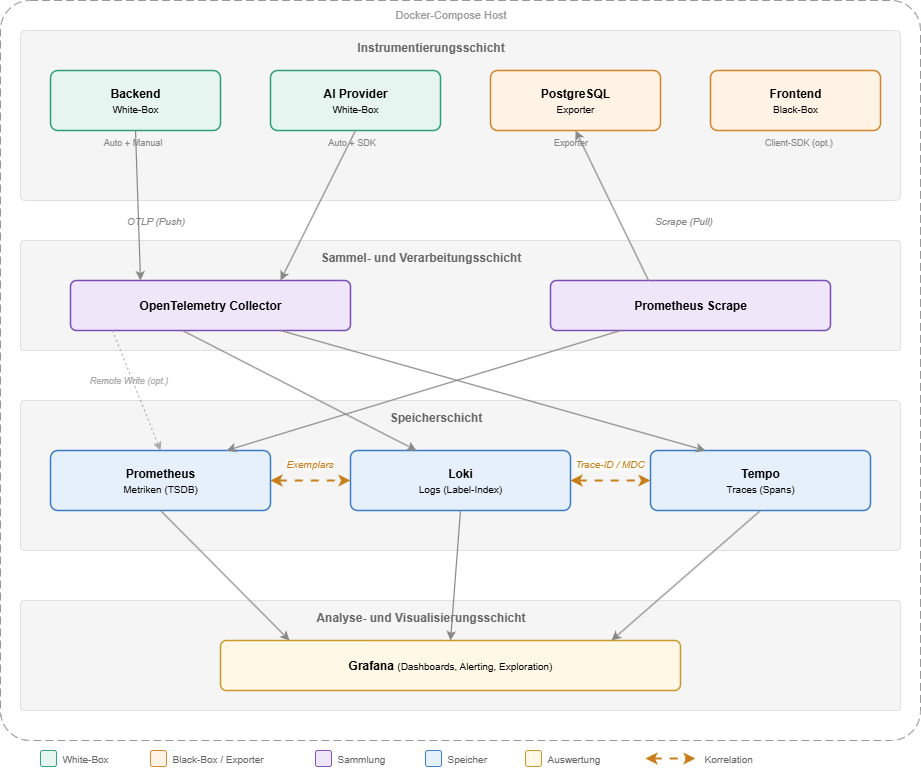
\includegraphics[width=0.95\textwidth]{images/fig_zielarchitektur.png}
\caption[Logische Zielarchitektur der Observability-Pipeline fuer frag.jetzt]{Logische Zielarchitektur der Observability-Pipeline fuer frag.jetzt. Gestrichelte Querverbindungen kennzeichnen Korrelationsmechanismen zwischen den Speicher-Backends. \small Quelle: Eigene Darstellung.}
\label{fig:zielarchitektur-observability}
\end{figure}


\subsection{Instrumentierungsschicht}
 
Aus der Architektur von frag.jetzt ergibt sich eine differenzierte Instrumentierungsstrategie. Backend, WebSocket Gateway und AI Provider sind als Eigenentwicklungen über Auto-Instrumentierung mit selektiver manueller Ergänzung beobachtbar. Die Quellcodeanalyse in Kapitel~3 hat gezeigt, dass keine dieser Komponenten bislang Telemetrie emittiert (R3). Demgegenüber agieren die externen LLM-Provider als Black-Box-Abhängigkeiten, bei denen mindestens die Ein- und Ausgangsseite jedes Aufrufs instrumentiert werden muss \parencite[S.~31]{bissig2024unified}.
 
OpenTelemetry übernimmt die Rolle der standardisierten Instrumentierungsschicht (vgl.~Abschnitt~5.2). Die entscheidenden Übergabepunkte für die Kontextpropagation sind die Verbindungen zwischen Frontend und Reverse-Proxy, zwischen Reverse-Proxy und Backend, zwischen Backend und Datenbank sowie zwischen Backend und AI Provider. Eine besondere Herausforderung stellt die Echtzeitkommunikation über den Message Broker dar, da dort eine manuelle Injektion des Trace-Kontexts in das Nachrichtenformat erforderlich wird \parencite[S.~25]{sundstrom2025finding}. Ergänzend werden Container-Metriken und datenbankspezifische Indikatoren über spezialisierte Exporter erhoben, die Prometheus-kompatible Endpunkte bereitstellen.
 
 
\subsection{Sammel- und Verarbeitungsschicht}
 
Der OpenTelemetry Collector fungiert als zentrale Routing-Komponente, die Instrumentierung und Backend entkoppelt \parencite[S.~107]{sakinala2025observability}; \parencite[S.~502]{gudimetla2025transitioning}. Für frag.jetzt wird der Collector als pushbasierte Empfangskomponente für anwendungsseitige Traces und Metriken konfiguriert, weil ein Push-Modell bei einer zukünftigen Erweiterung keine Umstellung erfordert \parencite[S.~39]{bissig2024unified}. Infrastrukturmetriken folgen dagegen dem etablierten Pull-Modell über Prometheus-Scraping. Bei dem für frag.jetzt erwarteten geringen Datenvolumen kann zunächst auf Sampling verzichtet werden. Eine Anpassung ist erst dann vorgesehen, wenn das Telemetrievolumen die Speicherkapazität des Hosts belastet.
 
 
\subsection{Speicherschicht}
 
Die aufbereiteten Signale werden in drei spezialisierten Backends abgelegt: Metriken in der lokalen Prometheus-TSDB, Logs in Loki mit labelbasierter Indexierung und Traces in Tempo. Entscheidend ist die Korrelierbarkeit über die drei Speicher hinweg, die bei getrennter Speicherung nicht automatisch entsteht \parencite[S.~44]{bissig2024unified}. Drei Mechanismen bilden die diagnostischen Brücken: die Trace-ID als gemeinsamer Identifikator über alle drei Pfeiler, die Injektion der Trace-ID in den Mapped Diagnostic Context (MDC) des Logging-Frameworks \parencite[S.~20]{sundstrom2025finding} und Metriken-Exemplars, die den direkten Übergang von einem aggregierten Metrikwert zum zugehörigen Trace ermöglichen \parencite[S.~25]{bissig2024unified}; \parencite[S.~12]{albuquerque2025tracing}. Die Speichertrennung ist nur dann diagnostisch tragfähig, wenn diese Verknüpfungspfade von Beginn an in der Instrumentierung verankert werden.
 
 
\subsection{Analyse- und Visualisierungsschicht}
 
Grafana bildet die einheitliche Oberfläche für Abfrage, Visualisierung und Alarmierung aller gespeicherten Telemetriedaten \parencite[S.~16]{sundstrom2025finding}. Die Korrelation wird über Datenquellen-übergreifende Navigation hergestellt: Von einem auffälligen Metrikpunkt lässt sich über ein Exemplar direkt zum zugehörigen Trace springen, und aus einem Trace heraus führen verknüpfte Logabfragen zum relevanten Kontext.
 
 
\subsection{Einordnung im Kontext von frag.jetzt}
 
Die beschriebene Vier-Schichten-Architektur orientiert sich an Referenzmodellen für Kubernetes-basierte Umgebungen \parencite[S.~501]{gudimetla2025transitioning}. frag.jetzt weicht davon in drei Punkten ab. Erstens läuft das Ökosystem auf einem einzelnen Host, sodass der Collector nicht als Sidecar, sondern als eigenständiger Container betrieben wird. Zweitens fehlt ein Service Mesh, weshalb die Telemetrieerzeugung vollständig auf Anwendungsebene erfolgen muss. Drittens erlaubt das geringe Telemetrievolumen einen Verzicht auf Sampling und vorgelagerte Aggregation, erfordert aber eine bewusste Kapazitätsbeobachtung bei wachsendem Einsatz. Die Architektur hält den Einstieg bewusst schlank und lässt Erweiterungspfade wie Mimir für Langzeitmetriken oder Tail-Based Sampling offen, ohne die Grundstruktur zu verändern \parencite[S.~1--2]{borges2024informed}.
 
 
\section{Servicebezogene Operationalisierung der Four Golden Signals}
\label{sec:golden-signals-operationalisierung}
 
Die Ableitung der Beobachtungsgrößen folgt dem in Abschnitt~4.2 beschriebenen Vorgehen und konzentriert sich auf die vier für die Forschungsfragen zentralen Beobachtungseinheiten: Frontend, Backend, Datenbank und externe KI-Dienste. Nginx, RabbitMQ und das WebSocket Gateway werden als Infrastruktur- bzw.\ Integrationskomponenten über die Infrastrukturmetriken mitbeobachtet, erhalten aber keine eigenständige Signal-Matrix. \textcite[S.~60]{ewaschukMonitoringDistributedSystems} bezeichnet die Wahl des Traffic-Indikators ausdrücklich als \emph{high-level system-specific metric}, was bedeutet, dass die Übertragung der vier Dimensionen auf jeden Dienst eine eigenständige Entwurfsleistung erfordert. Tabelle~\ref{tab:signal-matrix} fasst die Ergebnisse dieser Ableitung in einer Signal-Matrix zusammen. Die folgenden Unterabschnitte erläutern nur die Besonderheiten, die sich nicht unmittelbar aus der Matrix erschließen.
 
 
\subsection{PWA-Frontend}
\label{sec:gs-frontend}
 
Das Angular-Frontend unterscheidet sich grundlegend von den serverseitigen Komponenten, weil die Ausführung im Browser stattfindet und die Infrastruktur nicht direkt kontrollierbar ist. Aus Nutzersicht manifestiert sich Latenz als wahrgenommene Ladezeit, zu der neben der Server-Antwortzeit auch clientseitige Faktoren wie Netzwerkqualität und Rendering beitragen. Basisindikatoren sind die Dauer von API-Aufrufen und die Ende-zu-Ende-Ladezeit beim Betreten eines Raums. Browserbasierte Metriken wie First Contentful Paint über das OpenTelemetry-Browser-SDK sind als optionale Erweiterung zu verstehen.
 
Die Nachfrageintensität lässt sich über aktive WebSocket-Verbindungen und HTTP-Anfragen pro Zeiteinheit messen. Fehlerindikatoren umfassen fehlgeschlagene API-Aufrufe (4xx/5xx), unbehandelte JavaScript-Exceptions und WebSocket-Verbindungsabbrüche. Klassische Sättigungsmetriken wie CPU und Speicher beziehen sich auf das Endgerät und liegen außerhalb des Einflussbereichs des Betriebsteams. Da die Grenzen der Frontend-Beobachtbarkeit eng gesteckt sind, liegt der instrumentierungstechnische Schwerpunkt auf den serverseitigen Komponenten.
 
 
\subsection{Spring-Boot-Backend}
\label{sec:gs-backend}
 
Das Backend ist die zentrale Verarbeitungskomponente und der in Kapitel~3 identifizierte kritische Punkt. Der primäre Latenzindikator ist die Antwortdauer je REST-Endpunkt als Histogramm (p50, p95, p99), weil Durchschnittswerte die Erfahrung langsam bedienter Nutzer verbergen können \parencite[S.~60]{ewaschukMonitoringDistributedSystems}. Ebenso muss die Latenz erfolgreicher und fehlgeschlagener Anfragen getrennt erfasst werden, da schnell zurückgegebene Fehler den Gesamtdurchschnitt verzerren. Ergänzend werden die Latenzen ausgehender Aufrufe an PostgreSQL, den Message Broker und den AI Provider separat erhoben. Das reaktive Programmiermodell auf Basis von WebFlux erfordert dabei besondere Aufmerksamkeit, da die Messung auf Span-Ebene innerhalb der reaktiven Kette erfolgen muss \parencite[S.~25]{sundstrom2025finding}.
 
Die Anfragerate pro Endpunkt bildet den Traffic ab. Für die geschäftskritischen Abläufe aus Abschnitt~3.3 ist eine gesonderte Erfassung sinnvoll. Fehler werden auf mehreren Ebenen erfasst: HTTP-5xx-Statuscodes, unbehandelte Exceptions und fehlgeschlagene Downstream-Aufrufe. Da kein externer Aufruf einen Timeout besitzt (R1), äußern sich Timeout-bedingte Fehler als hängende Anfragen, was die Latenzüberwachung umso dringlicher macht. Die Sättigung wird über Container-Metriken und den R2DBC-Connection-Pool gemessen. \textcite[S.~60--61]{ewaschukMonitoringDistributedSystems} empfiehlt, Sättigung indirekt über steigende Latenz am 99.\,Perzentil zu erkennen, weil Latenzzunahmen häufig ein Frühindikator für Ressourcenerschöpfung sind.
 
 
\subsection{PostgreSQL}
\label{sec:gs-postgresql}
 
Die Datenbank ist an allen drei geschäftskritischen Nutzungspfaden beteiligt. Die Vote-Trigger und die Comment-Nummern-Generierung (Abschnitt~3.3) erzeugen potenzielle Engpässe. Der zentrale Latenzindikator ist die Abfrageausführungszeit, wobei lang laufende Abfragen auf fehlende Indizes oder Row-Level Contention hindeuten. Die Transaktionsrate und die aktive Verbindungszahl bilden den Traffic ab. Relevante Fehlersignale umfassen Deadlocks, fehlgeschlagene Transaktionen und Verbindungsablehnungen. Die Sättigung wird über das Verhältnis genutzter zu maximal verfügbarer Verbindungen, die Buffer-Cache-Hit-Rate und die Disk-I/O-Auslastung gemessen. Ein sinkender Cache-Hit-Anteil deutet darauf hin, dass die Arbeitsspeicherkonfiguration nicht mehr zum Datenvolumen passt.
 
 
\subsection{Externe KI-Dienste}
\label{sec:gs-ki}
 
Die Beobachtung der externen KI-Dienste beschränkt sich auf die Schnittstelle zwischen AI Provider und den angebundenen Modellen, da der Quellcode der LLM-Provider nicht verfügbar ist \parencite[S.~31]{bissig2024unified}. Die LLM-Antwortzeit wird als Histogramm pro Provider und Modell erfasst. Da kein Timeout konfiguriert ist (R1), kann ein einzelner hängender Aufruf den AI Provider blockieren und über die Aufrufkette das Backend beeinflussen. Der Traffic wird als Anzahl der LLM-Aufrufe pro Zeiteinheit je Funktionstyp gemessen. Fehlersignale sind HTTP-Fehlerantworten der Provider-APIs (insbesondere 429 Rate Limit Exceeded), Timeouts und Parsing-Fehler. Neun von 19~LLM-Providern sind explizit mit \texttt{max\_retries=0} konfiguriert, sodass ein fehlgeschlagener Aufruf unmittelbar durchschlägt. Da die LLM-Provider keinen Einblick in ihre Ressourcenauslastung gewähren, wird Sättigung über Proxy-Indikatoren wie steigende Antwortzeiten und zunehmende Rate-Limit-Fehler abgebildet.
 
 
\section{Serviceübergreifende Signal-Matrix}
\label{sec:signal-matrix}
 
Tabelle~\ref{tab:signal-matrix} verdichtet die vorangehenden Ableitungen in einer Gesamtübersicht. Sie bildet die Grundlage für das rollenbasierte Dashboard-Design (Abschnitt~6.5) und definiert den Rahmen für das Alerting-Konzept (Abschnitt~6.6), weil nicht jede Messgröße Alarmrelevant ist.
 
\begin{table}[htb]
\centering
\caption[Serviceübergreifende Signal-Matrix mit Zuordnung von Dienst, Golden Signal, Messgröße, Erhebungszweck und primärer Stakeholder-Rolle.]{Serviceübergreifende Signal-Matrix mit Zuordnung von Dienst, Golden Signal, Messgröße, Erhebungszweck und primärer Stakeholder-Rolle. \small Quelle: Eigene Darstellung.}
\label{tab:signal-matrix}
\small
\begin{tabularx}{\textwidth}{
  >{\RaggedRight\arraybackslash}p{1.6cm}
  >{\RaggedRight\arraybackslash}p{1.5cm}
  >{\RaggedRight\arraybackslash}p{5.9cm}
  >{\RaggedRight\arraybackslash}X
  >{\RaggedRight\arraybackslash}p{1.8cm}
}
\toprule
\textbf{Dienst} & \textbf{Signal} & \textbf{Messgröße} & \textbf{Zweck} & \textbf{Rolle} \\
\midrule
Backend   & Latency    & Antwortdauer je Endpunkt (p50, p95, p99)         & Nutzererfahrung, Engpasserkennung   & Entwicklung \\
Backend   & Traffic    & Anfragen/s je Pfad, Broker-Nachrichten/s          & Lastbild, Kapazitätsplanung         & DevOps \\
Backend   & Errors     & HTTP-5xx-Rate, Exception-Rate, Downstream-Fehler  & Fehlererkennung, Trendanalyse       & Entwicklung \\
Backend   & Saturation & CPU, Speicher, R2DBC-Pool-Nutzung                 & Ressourcenwarnung                   & DevOps \\[4pt]
PostgreSQL & Latency   & Abfrageausführungszeit (Durchschnitt, Maximum)     & Indexbedarf, Contention-Erkennung   & Entwicklung \\
PostgreSQL & Traffic   & Transaktionen/s, aktive Verbindungen               & Nutzungsintensität                  & DevOps \\
PostgreSQL & Errors    & Deadlocks, fehlgeschl.\ Transaktionen, Lock-Waits  & Stabilitätsüberwachung              & Entwicklung \\
PostgreSQL & Saturation & Verbindungspool-Quote, Cache-Hit-Rate, Disk-I/O   & Kapazitätswarnung                   & DevOps \\[4pt]
AI Prov.  & Latency    & LLM-Antwortzeit je Provider/Modell (Histogramm)    & SLA-Proxy, Kaskadenerkennung       & Entwicklung \\
AI Prov.  & Traffic    & LLM-Aufrufe/Zeiteinheit je Funktionstyp            & Nutzungsmuster, Kontingentplanung  & Product Owner \\
AI Prov.  & Errors     & Provider-Fehlerrate, 429er-Rate, Parsing-Fehler   & Verfügbarkeit ext.\ Abhängigkeiten & Entwicklung \\
AI Prov.  & Saturation & Antwortzeit-Trend, Rate-Limit-Häufigkeit, lokale CPU & Kapazitätswarnung               & DevOps \\[4pt]
Frontend  & Latency    & API-Aufruf-Dauer, Raum-Ladezeit                    & Nutzererfahrung                    & Product Owner \\
Frontend  & Traffic    & Aktive WS-Verbindungen, HTTP-Anfragen/s            & Nutzungsgrad                       & Product Owner \\
Frontend  & Errors     & HTTP-Fehler, JS-Exceptions, WS-Abbrüche           & Fehlererkennung clientseitig       & Entwicklung \\
Frontend  & Saturation & Antwortzeit-Trend, Retry-Häufigkeit                & Überlastindikation                 & DevOps \\
\bottomrule
\end{tabularx}
\end{table}
 
 
\section{Rollenbasiertes Informations- und Dashboard-Konzept}
\label{sec:dashboard-konzept}
 
Für frag.jetzt wird eine hierarchische Informationsarchitektur in drei Sichtebenen umgesetzt, deren Zuschnitt sich aus den Stakeholder-Gruppen und der Signal-Matrix ableitet \parencite[S.~108]{sakinala2025observability}.
 
\paragraph{Übersichtssicht (Product Owner / Management).}
Diese Ebene beantwortet die Frage, ob frag.jetzt aus Nutzersicht funktioniert. Sie zeigt verdichtete Indikatoren wie aktive Raumsitzungen, globale Fehlerrate und Gesamtlatenz der Kernabläufe. Detailinformationen sind nur über Verlinkung erreichbar.
 
\paragraph{Dienst- und Infrastruktursicht (DevOps / Betrieb).}
Diese Ebene beantwortet die Frage, wo das Problem liegt. Sie stellt Ressourcenmetriken je Container, Datenbankauslastung, Message-Broker-Kennzahlen und eine aus Trace-Daten gewonnene Service-Map dar.
 
\paragraph{Diagnose- und Entwicklungssicht (Entwicklung).}
Diese Ebene beantwortet die Frage, was genau im Code passiert. Sie bietet endpunktbezogene Latenzhistogramme, Fehleraufschlüsselungen, Trace-Ansichten und die Möglichkeit, aus einem Trace in die zugehörigen Logeinträge zu springen. Die technische Umsetzung wird in Kapitel~7 dokumentiert.
 
 
\section{Alerting-Konzept und Runbook-Logik}
\label{sec:alerting-konzept}
 
Aufbauend auf den in Abschnitt~2.7 erarbeiteten Grundlagen folgt das Alerting-Konzept drei Grundsätzen. Alarme reagieren symptomorientiert auf nutzerwirksame Zustände statt auf interne Ursachenindikatoren \parencite[S.~63--64]{ewaschukMonitoringDistributedSystems}. Jeder Alarm muss handlungsfähig sein, also Problem, betroffene Komponente und empfohlene Erstmaßnahme erkennbar machen \parencite[S.~174]{vinnakota2025creating}. Schweregrade orientieren sich an der Nutzerwirkung: \emph{Critical} für akute Ausfälle geschäftskritischer Funktionen, \emph{Warning} für sich abzeichnende Verschlechterungen.
 
 
\subsection{Alarmkategorien}
 
Aus der Signal-Matrix lassen sich vier Kategorien ableiten. Die konkreten Schwellenwerte und Zeitfenster werden in Kapitel~7 festgelegt.
 
\paragraph{Verfügbarkeitsalarme (Critical).}
Ein Alarm wird ausgelöst, wenn eine geschäftskritische Funktion nicht mehr erreichbar ist, etwa wenn das Backend über einen definierten Zeitraum keine erfolgreichen Antworten liefert oder die Datenbankverbindung dauerhaft fehlschlägt.
 
\paragraph{Latenzalarme (Warning / Critical).}
Steigt die Antwortzeit eines Kernendpunkts über einen definierten Grenzwert, etwa das 95.\,Perzentil über ein gleitendes Fenster, wird zunächst eine Warnung und bei weiterer Verschlechterung ein kritischer Alarm erzeugt. Für die KI-Dienste gelten angepasste Grenzwerte.
 
\paragraph{Fehleralarme (Warning / Critical).}
Eine Fehlerrate oberhalb eines definierten Anteils löst eine Warnung aus. Die explizite Trennung von client- (4xx) und serverseitigen (5xx) Fehlern verhindert, dass ungültige Eingaben denselben Alarm wie interne Serverfehler erzeugen.
 
\paragraph{Sättigungsalarme (Warning).}
Ressourcenmetriken wie CPU-Auslastung und Datenbankverbindungspool-Nutzung werden als vorausschauende Warnung konfiguriert. \textcite[S.~60--61]{ewaschukMonitoringDistributedSystems} empfiehlt, Sättigung indirekt über steigende Latenz am 99.\,Perzentil zu erkennen.
 
 
\subsection{Runbook-Verknüpfung}
 
Jeder Critical-Alarm wird mit einem Runbook verknüpft, das Problembeschreibung, betroffene Komponente, Diagnoseschritte, Erstmaßnahmen und Eskalationspfad enthält. Für den Prototyp werden exemplarische Runbooks für den Kaskadeneffekt durch KI-Service-Timeouts (R1) und Datenbankengpässe bei Massenabstimmungen (R2) erstellt.
 
\medskip
 
Regelbasierte Alarme stoßen an Grenzen, sobald sich Lastmuster im Tages- oder Semesterverlauf verändern und starre Schwellenwerte entweder zu viele False Positives oder zu späte Warnungen produzieren \parencite[S.~173]{vinnakota2025creating}. Anomaliebasierte Verfahren setzen jedoch ein trainiertes Modell des Normalverhaltens voraus, das für frag.jetzt mangels historischer Produktivdaten derzeit nicht existiert \parencite[S.~5--6]{soldani2022anomaly}. Die standardisierte Metrikerhebung über Prometheus und die offene Abfrageschnittstelle über PromQL erlauben es, solche Verfahren als zukünftigen Ausbauschritt ohne Änderung der Instrumentierung anzubinden.
 
% =============================================================================
% KAPITEL 7 – Prototypische Implementierung
% =============================================================================
 
\chapter{Prototypische Implementierung}
 
Dieses Kapitel dokumentiert die praktische Umsetzung der in Kapitel~6 konzipierten Observability-Strategie. Es beschreibt den Umfang des Prototyps, die Instrumentierung der Kernkomponenten, die beobachtete Funktionsfähigkeit in exemplarischen Szenarien, die Umsetzung eines Golden-Signals-Dashboards sowie die Konfiguration exemplarischer Alerting-Regeln mit zugehörigen Runbooks. Den Abschluss bildet eine Reflexion über Herausforderungen, die während der Implementierung aufgetreten sind.
 
 
\section{Umfang und Abgrenzung der prototypischen Umsetzung}
 
Die Umsetzung erfolgte auf dem Staging-Server von frag.jetzt, auf dem der vollständige Anwendungsstack in einer produktionsnahen Docker-Compose-Konfiguration betrieben wird. Der Observability-Stack wurde als eigenständiges Compose-Projekt neben der bestehenden Orchestrierung deployt und über ein gemeinsames Docker-Netzwerk an die Applikationscontainer angebunden.
 
Die Implementierung umfasst drei Schwerpunkte: erstens das Deployment des LGTM-Stacks mit allen Speicher-Backends und Infrastruktur-Exportern, zweitens die Instrumentierung von Backend und WS-Gateway über den OpenTelemetry Java Agent und drittens die Erstellung eines Golden-Signals-Dashboards in Grafana mit zugehörigen Alerting-Regeln. Bewusst ausgeklammert wurden die Instrumentierung des AI Providers (Python/FastAPI) und des Frontends (Angular/Nginx), die clientseitige Browser-Telemetrie sowie die Produktivhärtung mit Hochverfügbarkeit und Langzeitspeicherung. Ebenso beschränkt sich das Dashboard-Design auf ein einzelnes, technisch orientiertes Golden-Signals-Dashboard. Die in Kapitel~6.5 konzipierte rollenspezifische Aufbereitung für Product Owner und Entwicklung verbleibt als Ausbauschritt, weil sie auf denselben Datenquellen aufsetzt und primär eine Frage der Informationsverdichtung ist.
 
Diese Abgrenzungen begrenzen die Vollständigkeit der prototypischen Validierung: Eine durchgängige Ende-zu-Ende-Beobachtbarkeit aller Systemgrenzen kann ohne Frontend- und AI-Provider-Instrumentierung nicht nachgewiesen werden. Die Teilumsetzung erlaubt jedoch die Prüfung der zentralen Mechanismen, insbesondere der Trace-Erfassung über Dienstgrenzen, der Metrik-Aggregation entlang der Golden Signals und der Korrelation zwischen Telemetriesignalen. \textcite[S.~52]{bissig2024unified} beobachten in einer vergleichbaren Implementierungsstudie, dass der Hauptaufwand bei der Einführung von Observability nicht in der theoretischen Konzeption, sondern in den Infrastrukturentscheidungen und der Konfiguration der Observability-Komponenten liegt.
 
Die folgenden Abschnitte dokumentieren die konkreten Konfigurationen und ihre beobachteten Ergebnisse. Umfangreichere Konfigurationsdateien wie die vollständige OTel-Collector-Konfiguration und das Dashboard-JSON befinden sich im Anhang.
 
 
\section{Instrumentierung ausgewählter Kernkomponenten}
\label{sec:instrumentierung}
 
Die Instrumentierung folgt dem in Kapitel~6.2 beschriebenen Schichtenmodell: Applikationsdienste senden Telemetriedaten über OTLP an den Collector, Infrastrukturkomponenten werden über dedizierte Exporter beobachtet. Tabelle~\ref{tab:instrumentierung-uebersicht} gibt eine Übersicht über die instrumentierten Komponenten, die jeweils erzeugten Signale und den im Prototyp beobachteten Nachweis.
 
\begin{table}[ht]
\centering
\caption{Übersicht der instrumentierten Komponenten und beobachteten Telemetriesignale.}
\label{tab:instrumentierung-uebersicht}
\small
\begin{tabularx}{\textwidth}{
  >{\RaggedRight\arraybackslash}p{2.2cm}
  >{\RaggedRight\arraybackslash}p{2.5cm}
  >{\RaggedRight\arraybackslash}X
  >{\RaggedRight\arraybackslash}X
}
\toprule
\textbf{Komponente} & \textbf{Instrumentierung} & \textbf{Erzeugte Signale} & \textbf{Nachweis im Prototyp} \\
\midrule
Backend (Spring Boot) & OTel Java Agent (Auto-Instr.) & HTTP-Spans, DB-Spans, Logback-Logs mit Trace-ID, JVM-Metriken & Span-Waterfall mit DB-Operationen in Grafana sichtbar \\[4pt]
WS-Gateway (Netty) & OTel Java Agent (Auto-Instr.) & WebSocket-Spans, RabbitMQ-Spans, JVM-Metriken & Service Graph zeigt Knoten mit Anfragerate \\[4pt]
PostgreSQL & PostgreSQL Exporter & Verbindungszähler, Transaktionsraten, Lock-Statistiken & \texttt{pg\_stat\_activity\_count} in Prometheus abfragbar \\[4pt]
RabbitMQ & Prometheus-Plugin & Queue-Tiefen, Nachrichten\-raten & \texttt{rabbitmq\_queue\_messages} in Dashboard-Panel sichtbar \\[4pt]
Host & Node Exporter, cAdvisor & CPU, Speicher, Netzwerk, Container-Metriken & Gauge-Panels im Dashboard mit Schwellenwertfärbung \\
\bottomrule
\end{tabularx}
\end{table}
 
 
\subsection{Observability-Stack und Telemetrie-Pipeline}
 
Das Deployment umfasst acht Container, die über ein separates Docker-Compose-File orchestriert werden. Der OpenTelemetry Collector empfängt sämtliche Applikationstelemetrie über OTLP (gRPC auf Port~4317, HTTP auf Port~4318) und verteilt sie an die drei Speicher-Backends: Metriken an Prometheus, Logs an Loki und Traces an Tempo. Für die Infrastrukturschicht erfassen cAdvisor Container-Ressourcenmetriken, der Node Exporter Host-Kennzahlen und der PostgreSQL Exporter Datenbankmetriken. Die Metriken des RabbitMQ-Prometheus-Plugins werden von Prometheus direkt über das Docker-interne Netzwerk abgerufen, ohne dass ein zusätzlicher Port auf dem Host freigegeben werden muss. Damit implementiert die Pipeline das in Kapitel~6.2 entworfene Architekturschema mit den dort festgelegten Komponentenzuordnungen.
 
Alle Observability-Container sind mit expliziten Speicherlimits konfiguriert, um das in Kapitel~3 beschriebene Risiko einer unkontrollierten Ressourcenverdrängung (R5) nicht im Observability-Stack selbst zu reproduzieren. Grafana wird mit provisionierten Datenquellen gestartet, sodass Prometheus, Loki und Tempo beim ersten Aufruf bereits konfiguriert sind. Die Datenquellen-Provisioning stellt insbesondere die Verknüpfungen zwischen den Backends her: Tempo-Traces können auf korrespondierende Loki-Logs verweisen und umgekehrt. Diese Korrelationsfähigkeit ist eine Voraussetzung für die in A1 geforderte Ende-zu-Ende-Nachvollziehbarkeit \parencite[S.~16]{sundstroem2025faults}.
 
 
\subsection{Applikationsinstrumentierung über den OTel Java Agent}
 
Für die JVM-basierten Dienste (Backend und WS-Gateway) wurde der OpenTelemetry Java Agent in Version~2.26.0 eingesetzt. Der Agent wird nicht in das Docker-Image integriert, sondern als Read-Only-Volume in den Container gemountet und über die Umgebungsvariable \texttt{JAVA\_TOOL\_OPTIONS} als JVM-Argument aktiviert. Dieser Ansatz vermeidet Änderungen am Applikationscode und an den bestehenden Docker-Images. \textcite[S.~51--52]{bissig2024unified} bestätigen, dass bei Standard-Java-Diensten lediglich das Einbinden des Agenten als Volume und die Konfiguration weniger Umgebungsvariablen erforderlich sind, um funktionsfähige Telemetrie zu erzeugen. Die Konfiguration erfolgt vollständig über Umgebungsvariablen im Docker-Compose-Override-File: Dienstname (\texttt{OTEL\_SERVICE\_NAME}), Collector-Adresse (\texttt{OTEL\_EXPORTER\_OTLP\_ENDPOINT}), Exportformat und Umgebungsattribute.
 
Der Agent instrumentiert automatisch HTTP-Anfragen (Spring WebFlux, Netty), R2DBC-Datenbankzugriffe, RabbitMQ-Interaktionen und Logback-Logausgaben. Im Ergebnis erzeugt jeder eingehende HTTP-Request einen Root-Span, der untergeordnete Spans für Datenbankoperationen enthält. Die Trace-Ansicht in Grafana zeigt diese Hierarchie als Span-Waterfall, in der beispielsweise ein \texttt{POST /livepoll/find}-Request mit seinen zugehörigen \texttt{SELECT}- und \texttt{UPDATE}-Operationen auf der PostgreSQL-Datenbank sichtbar wird. Für die instrumentierten Dienste ist damit der Verarbeitungspfad vom HTTP-Eingang über die Geschäftslogik bis zur Datenpersistierung in einem zusammenhängenden Trace rekonstruierbar, was Anforderung~A1 in Teilen adressiert.
 
[HIER MÖGLICHES BILD EINFÜGEN: Span-Waterfall eines Backend-Trace mit DB-Spans (POST /livepoll/find, 13 Spans, 15.4~ms)]
 
Der Service Graph in Grafana, der aus den von Tempo generierten Span-Metriken gespeist wird, visualisiert die Kommunikationsbeziehungen zwischen den instrumentierten Diensten. Im Prototyp zeigt er drei Knoten (\texttt{fragjetzt-backend}, \texttt{fragjetzt-ws-gateway} und \texttt{fragjetzt-postgres}) mit ihren jeweiligen Anfrageraten und durchschnittlichen Antwortzeiten. Die automatische Erzeugung dieses Graphen aus Trace-Daten bestätigt, dass die gewählte Kombination aus OTel Agent und Tempo die in Kapitel~5 als Vorteil beschriebene enge Grafana-Integration im Prototyp einlöst \parencite[S.~16]{sundstroem2025faults}.
 
[HIER MÖGLICHES BILD EINFÜGEN: Service Graph mit user → backend → postgres und user → ws-gateway]
 
 
\subsection{Infrastrukturexporter und Scrape-Konfiguration}
 
Prometheus scrapt sechs Targets im 15-Sekunden-Intervall: sich selbst, den OTel Collector, cAdvisor, den Node Exporter, den PostgreSQL Exporter und das RabbitMQ-Prometheus-Plugin. Die Infrastruktur-Exporter liefern Metriken, die direkt auf die Sättigungsindikatoren der Signal-Matrix aus Kapitel~6.4 abbilden: \texttt{pg\_stat\_activity\_count} für die Datenbankverbindungsauslastung, \texttt{rabbitmq\_queue\_messages} für Queue-Tiefen, \texttt{node\_memory\_MemAvailable\_bytes} für die Host-Speicherauslastung und JVM-Metriken (\texttt{jvm\_memory\_used\_bytes}, \texttt{jvm\_cpu\_recent\_utilization\_ratio}) für die Anwendungsressourcen. Damit wird Anforderung~A5 auf Metrikebene im Prototyp abgebildet.
 
Ergänzend zu den Infrastrukturmetriken empfängt Prometheus über den OTLP-Receiver Applikationsmetriken vom OTel Collector, darunter HTTP-Request-Dauer-Histogramme (\texttt{http\_server\_request\_duration\_seconds}). Tempo generiert aus den eingehenden Traces automatisch Span-Metriken (\texttt{traces\_spanmetrics\_calls\_total}, \texttt{traces\_spanmetrics\_latency}) und schreibt diese per Remote Write an Prometheus zurück. Aus diesen Span-Metriken werden der Service Graph und die Traffic- sowie Fehlerratenpanels im Dashboard gespeist. Dieses Zusammenspiel aus Infrastruktur- und Applikationsmetriken entspricht den von \textcite[S.~10, 16]{albuquerque2025tracing} beschriebenen komplementären Entwurfsmustern \emph{Application Metrics} und \emph{Infrastructure Metrics}.
 
 
\subsection{Logging-Anbindung}
 
Das Backend erzeugte im Standardbetrieb nahezu keine Logausgaben, weil Spring Boot WebFlux eingehende HTTP-Requests nicht automatisch protokolliert. Die Logs, die über den OTel Agent an Loki weitergeleitet werden, beschränkten sich auf Startmeldungen. Für den Prototyp wurde Debug-Level-Logging für die HTTP-Verarbeitungsschicht (\texttt{org.springframework.web}) selektiv aktiviert, sodass auch Request-bezogene Einträge in Loki verfügbar sind und über die vom OTel Agent automatisch injizierten Trace-IDs mit den zugehörigen Spans korreliert werden können. Diese Korrelierbarkeit über Trace-IDs adressiert Anforderung~A3 in Grundzügen.
 
Einschränkend ist festzuhalten, dass diese Konfiguration eine Demonstrationslösung für den Staging-Prototyp darstellt. Debug-Level-Logging erzeugt ein hohes Ausgabevolumen, das im Produktivbetrieb nicht vertretbar wäre. Für einen späteren Produktiveinsatz wäre stattdessen strukturierte, selektiv priorisierte JSON-Protokollierung vorzuziehen, bei der Logeinträge je nach Schweregrad gefiltert und nur geschäftsrelevante Ereignisse dauerhaft an Loki weitergeleitet werden.
 
 
\subsection{Exemplarische Validierungsszenarien}
\label{sec:validierung}
 
Um die Funktionsfähigkeit der Telemetrie-Pipeline über die reine Konfigurationsbeschreibung hinaus zu belegen, wurden drei Szenarien auf dem Staging-Server exemplarisch durchgeführt. Die Szenarien folgen jeweils dem Muster: Ausgangsaktion, erwartete Telemetriesignale, beobachtetes Ergebnis. Sie erheben keinen Anspruch auf systematische Testabdeckung, sondern dienen als Plausibilitätsnachweis für die Kernmechanismen.
 
\paragraph{Szenario 1: Normaler Nutzerrequest (Frage stellen).}
Ein Nutzer erstellte über die Weboberfläche eine neue Frage in einem aktiven Raum. Erwartet wurde ein Root-Span für den \texttt{POST /comment/}-Endpunkt mit untergeordneten Spans für den Datenbank-Insert sowie ein Anstieg des Latenz- und Traffic-Panels im Dashboard. In Grafana war der entsprechende Trace mit 8~Spans sichtbar, darunter der \texttt{INSERT}-Span auf der PostgreSQL-Datenbank mit einer Dauer von 3,2\,ms. Das Dashboard zeigte für den betreffenden Endpunkt im betrachteten Zeitfenster ein p50-Latenzniveau von circa 12\,ms. Damit stimmen die aggregierte Metriksicht und die beobachtete Größenordnung des Einzeltraces plausibel überein. Dieses Ergebnis bestätigt, dass die in A1 geforderte Nachvollziehbarkeit für die instrumentierten Dienste funktional gegeben ist.
 
\paragraph{Szenario 2: Erhöhte Last auf Voting-Endpunkt.}
Durch wiederholte manuelle Abstimmungen auf mehrere Fragen wurde eine erhöhte Anfragerate auf dem \texttt{POST /vote/}-Endpunkt erzeugt. Erwartet wurde ein sichtbarer Anstieg im Traffic-Panel und ein messbarer Effekt auf die Datenbankverbindungsauslastung. Im Dashboard stieg die Anfragerate des Backends im Beobachtungszeitraum erkennbar an. Der PostgreSQL-Verbindungszähler (\texttt{pg\_stat\_activity\_count}) blieb im unkritischen Bereich, was bei manueller Last erwartbar ist. Das Szenario zeigt, dass Sättigungsindikatoren (A5) unter Last prinzipiell sichtbar werden, auch wenn ein belastbarer Stresstest ein automatisiertes Lastwerkzeug erfordern würde.
 
\paragraph{Szenario 3: Provozierter Fehlerfall.}
Ein HTTP-Request an einen nicht existierenden Endpunkt (\texttt{GET /api/nonexistent}) erzeugte einen 404-Statuscode. In Tempo war der zugehörige Trace mit einem Fehler-Tag (\texttt{http.status\_code=404}) sichtbar. Im Errors-Panel des Dashboards erschien der Endpunkt in der Tabelle der fehlerhäufigsten Span-Operationen. Der Critical-Alert für die HTTP-5xx-Fehlerrate wurde durch dieses Szenario nicht ausgelöst, weil der Prototyp ausschließlich 5xx-Fehler als kritisch wertet. Ein gezielter Test des 5xx-Alerts, etwa durch temporäres Abschalten der Datenbank, wurde im Rahmen der prototypischen Umsetzung nicht durchgeführt und wäre für eine weitergehende Validierung empfehlenswert.
 
\medskip
 
Die drei Szenarien demonstrieren, dass Traces, Metriken und Logs im Prototyp tatsächlich erzeugt, gespeichert und im Dashboard dargestellt werden. Sie belegen die grundlegende Funktionsfähigkeit der Pipeline, ersetzen jedoch keine systematische Last- oder Fehlerinjektionsprüfung, wie sie für eine Produktivfreigabe erforderlich wäre.
 
 
\section{Umsetzung des Golden-Signals-Dashboards}
 
Das Golden-Signals-Dashboard wurde als Grafana-JSON-Modell erstellt und über den Import-Mechanismus in die Grafana-Instanz geladen. Es enthält 15~Panels in fünf Sektionen, die den vier Golden Signals und einer Infrastruktursektion entsprechen. Die Panelstruktur bildet die in Kapitel~6.4 definierte Signal-Matrix ab und übersetzt die dort festgelegten Messgrößen in konkrete Visualisierungen. Im Folgenden wird für jede Sektion erläutert, welches Diagnoseziel sie verfolgt und welche Prometheus-Abfragefamilien die Panels speisen.
 
Die Sektion \emph{Latency} zeigt Backend-Antwortzeiten als Perzentil-Zeitreihen (p50, p95, p99) und eine aufgeschlüsselte Latenzansicht pro HTTP-Endpunkt. Die Panels basieren auf dem Histogramm \texttt{http\_server\_request\_duration\_seconds\_bucket} und nutzen die Prometheus-Funktion \texttt{histogram\_quantile}. Die Perzentildarstellung folgt dem Prinzip, dass eine rein arithmetisch gemittelte Latenz langsame Anfragen verbergen kann \parencite[S.~7]{ewaschukMonitoringDistributedSystems}. Die endpunktspezifische Aufschlüsselung ermöglicht es, Pfade wie \texttt{/livepoll/find} oder \texttt{/comment/} gezielt zu beobachten. Das Diagnoseziel dieser Sektion besteht darin, zwischen einer globalen Verlangsamung und endpunktspezifischen Ausreißern zu unterscheiden, was für die Nachverfolgung der User Journeys aus Kapitel~3.3 nützlich ist.
 
Die Sektion \emph{Traffic} stellt die Anfragerate pro Dienst aus Span-Metriken (\texttt{traces\_spanmetrics\_calls\_total}) sowie die meistfrequentierten Endpunkte als gestapeltes Balkendiagramm dar. Das Diagnoseziel ist die Sichtbarkeit von Lastverteilung und Lastspitzen. Im Kontext von frag.jetzt macht diese Darstellung sichtbar, ob etwa Voting-Endpunkte unter Spitzenlast dominieren, was auf die in R2 beschriebene Row-Level Contention hindeuten könnte.
 
Die Sektion \emph{Errors} kombiniert eine Span-basierte Fehlerrate pro Service mit einem Stat-Panel für die HTTP-5xx-Quote und einer Tabelle der fehlerhäufigsten Span-Operationen. Diese Kombination verfolgt ein gestuftes Diagnoseziel: Das Stat-Panel zeigt, \emph{ob} ein Fehlerproblem vorliegt, die Tabelle zeigt, \emph{wo} es auftritt, und über den Trace-Link lässt sich der Kontext des fehlerhaften Requests in Tempo aufrufen.
 
Die Sektion \emph{Saturation} umfasst JVM-Heap-Auslastung, Thread-Zähler und CPU-Nutzung als Gauge-Panel mit Schwellenwertfärbung. Die Schwellenwerte orientieren sich an den in Kapitel~6.4 festgelegten initialen Startwerten (beispielsweise 80\,\% Heap-Auslastung als Warngrenze). Das Diagnoseziel ist die frühzeitige Erkennung von Ressourcenengpässen, bevor sie sich als Latenzanstieg oder Fehlerrate in den anderen Sektionen manifestieren.
 
Die \emph{Infrastruktur}-Sektion zeigt PostgreSQL-Verbindungen (\texttt{pg\_stat\_activity\_count}), RabbitMQ-Queue-Tiefen (\texttt{rabbitmq\_queue\_messages}), Host-Ressourcen und GC-Pausen sowie den Service Graph aus Tempo. Die PostgreSQL-Panels adressieren den Sättigungsindikator der Datenbankkomponente, die in der Signal-Matrix als besonders kritisch bewertet wurde.
 
Sämtliche Panels verwenden \texttt{\$\_\_rate\_interval} als dynamisches Zeitfenster für Rate-Berechnungen, sodass die Darstellung sich automatisch an den gewählten Betrachtungszeitraum anpasst. Das Dashboard greift ausschließlich auf die in Abschnitt~7.2 beschriebenen Datenquellen zu und erfordert keine zusätzliche Konfiguration. Die vollständige JSON-Definition befindet sich in Anhang~[VERWEIS].
 
[HIER MÖGLICHES BILD EINFÜGEN: Screenshot des Golden-Signals-Dashboards mit befüllten Panels]
 
Das vorliegende Dashboard ist ein technisches Übersichtsdashboard, das primär DevOps-Aufgaben unterstützt. Die in Kapitel~6.5 konzipierten rollenspezifischen Sichten für Entwicklung und Product Owner wurden im Prototyp nicht umgesetzt. Sie ließen sich aus denselben Prometheus- und Loki-Datenquellen ableiten, indem die Informationsdichte und der Abstraktionsgrad der Panels angepasst werden.
 
 
\section{Alerting-Regeln und Beispiel-Runbooks}
 
Die in Kapitel~6.6 konzipierte Alerting-Logik wird exemplarisch in konkrete Grafana-Alerting-Regeln überführt. Die Regeln nutzen Grafana Unified Alerting, das Schwellenwertbedingungen auf Prometheus-Abfragen auswertet und bei Überschreitung Benachrichtigungen über konfigurierbare Kanäle auslöst. Im Prototyp wurde ein E-Mail-Kanal konfiguriert; für den Produktivbetrieb wären zusätzlich Integrationen in Messaging-Dienste oder PagerDuty vorgesehen. Die Umsetzung adressiert Anforderung~A4 (handlungsfähige Alarmierung).
 
Drei exemplarische Alerting-Regeln illustrieren die drei Schweregrade aus Kapitel~6.6:
 
Die erste Regel (\emph{Critical}) löst aus, wenn die HTTP-5xx-Fehlerrate des Backends über fünf Minuten den Schwellenwert von 5\,\% überschreitet. Die Prometheus-Abfrage berechnet den Anteil der 5xx-Antworten an allen Antworten über ein gleitendes Fenster. Ein Alarm auf dieser Ebene signalisiert eine nutzerwirksame Beeinträchtigung und erfordert sofortiges Eingreifen.
 
Die zweite Regel (\emph{Warning}) reagiert auf eine PostgreSQL-Verbindungsauslastung über 70\,\% des konfigurierten Limits von 100~Verbindungen. Der Schwellenwert basiert auf dem Indikator \texttt{pg\_stat\_activity\_count} im Verhältnis zur konfigurierten Maximalgröße. Ein wachsender Verbindungspool deutet auf einen bevorstehenden Engpass hin, der rechtzeitig adressiert werden kann.
 
Die dritte Regel (\emph{Warning}) überwacht die Backend-Latenz im p95-Bereich und alarmiert bei einer anhaltenden Überschreitung von 500\,ms über drei Minuten.
 
Alle drei Regeln folgen dem symptomorientierten Ansatz, der in der SRE-Literatur als Kern wirksamer Alerting-Konfigurationen beschrieben wird: Sie reagieren auf nutzerwirksame Zustände, nicht auf interne Ursachenindikatoren \parencite[S.~11--12]{ewaschukMonitoringDistributedSystems}. Die Evaluationsfenster von drei bis fünf Minuten fungieren als Debounce-Mechanismus, der transiente Spitzen toleriert und dadurch die Zahl falsch-positiver Alarme reduzieren soll \parencite[S.~176]{vinnakota2025creating}. Jede Regel enthält in ihrer Annotation-Konfiguration einen Link zum zugehörigen Runbook sowie zum relevanten Dashboard-Panel, sodass beim Eintreffen des Alarms der operative Kontext unmittelbar verfügbar ist. \textcite[S.~174]{vinnakota2025creating} betonen, dass jeder Alarm vier Fragen beantworten muss: Was ist betroffen? Warum vermutlich? Welche Sofortmaßnahme? Wer ist zuständig? Die Annotation-Links adressieren die ersten drei Fragen; die Zuständigkeitsfrage bleibt im Prototyp offen, da frag.jetzt derzeit kein formales On-Call-Modell betreibt.
 
Einschränkend ist zu vermerken, dass die drei Regeln im Prototyp angelegt und konfiguriert, aber nicht durch gezielte Störungsinjektionen systematisch verifiziert wurden. Die Plausibilisierung beschränkt sich auf das in Abschnitt~\ref{sec:validierung} beschriebene Fehlerszenario, bei dem der 5xx-Alert erwartungsgemäß \emph{nicht} auslöste. Ein belastbarer Test, etwa durch temporäres Abschalten der Datenbank oder künstliche Latenzinjektionen, wäre für eine weitergehende Validierung erforderlich.
 
Im Vergleich zu den in Kapitel~6.7 skizzierten anomaliebasierten Verfahren bleibt der Ansatz statisch: Die Schwellenwerte passen sich nicht automatisch an Lastschwankungen an, und es findet keine automatische Korrelation zwischen verschiedenen Alarmsignalen statt. \textcite[S.~173]{vinnakota2025creating} weisen darauf hin, dass starre Schwellwerte in dynamischen Umgebungen saisonale Muster und Abhängigkeiten zwischen Diensten unzureichend berücksichtigen. Für frag.jetzt mit seinen kalendergebundenen Lastspitzen während Vorlesungszeiten wäre eine spätere Ergänzung um dynamische Schwellen sinnvoll. Die konkreten Alerting-Definitionen im Grafana-JSON-Format befinden sich in Anhang~[VERWEIS].
 
Ergänzend wurden zwei Runbooks als strukturierte Markdown-Dokumente erstellt, die der in Kapitel~6.6 definierten Fünf-Felder-Struktur (Symptom, Kontext, Diagnose, Behebung, Eskalation) folgen. Das erste Runbook behandelt den Alarm "`Backend-Fehlerrate über Schwellenwert"' und verweist auf das Golden-Signals-Dashboard, die Trace-Suche in Tempo und die Logabfrage in Loki als Diagnoseressourcen. Es beschreibt als Behebungsschritte die Inspektion der jüngsten Traces auf fehlerhafte Spans, die Prüfung der Datenbankverbindungen und den Neustart des Backend-Containers als Sofortmaßnahme. Das zweite Runbook adressiert den Alarm "`PostgreSQL-Verbindungspool nahe Limit"' und leitet durch die Prüfung der aktiven Verbindungen über den PostgreSQL Exporter, die Identifikation langlaufender Queries und die Erhöhung der \texttt{max\_connections} als Kapazitätsmaßnahme. Beide Runbooks sind bewusst so formuliert, dass sie auch von Personen ohne tiefe frag.jetzt-Kenntnis nachvollzogen werden können. Die vollständigen Runbooks befinden sich im Anhang~[VERWEIS].
 
 
\section{Herausforderungen und Lösungen bei der Umsetzung}
 
Die prototypische Implementierung verlief nicht friktionsfrei. Drei Kategorien von Herausforderungen traten auf, die in vergleichbaren Deployments ebenfalls zu erwarten wären und daher hier dokumentiert werden.
 
 
\subsection{Ressourcendimensionierung}
 
Das Trace-Backend Tempo wurde initial mit einem Speicherlimit von 256\,MB konfiguriert. Unter der Trace-Last, die Backend und WS-Gateway über den OTel Agent erzeugten, erschöpfte der Container seinen verfügbaren Speicher und wurde wiederholt durch den Kernel beendet (OOM-Kill, Exit Code~137). Jeder erzwungene Neustart hinterließ unvollständige WAL-Dateien (Write-Ahead Log), die beim nächsten Start erneut Fehler verursachten. Die Lösung bestand aus zwei Schritten: der Erhöhung des Speicherlimits auf 512\,MB und der einmaligen Bereinigung des WAL-Volumes.
 
\textcite[S.~52]{bissig2024unified} berichten, dass Konfigurationsfehler bei Observability-Komponenten zu Datenverlust führen können und der operative Aufwand oft unterschätzt wird. Dieses Problem veranschaulicht zudem, dass die Ressourcendimensionierung von Observability-Komponenten auf einem Single-Host-System eine sorgfältige Abstimmung erfordert, insbesondere wenn die Anwendungscontainer bereits ohne Ressourcenlimits betrieben werden (vgl.~R5). Die Auto-Instrumentierung selbst erzeugt einen nicht trivialen Ressourcen-Overhead: \textcite[S.~50--51]{bissig2024unified} messen in einem Benchmark mit Java-Spring-Boot-Diensten einen CPU-Anstieg von rund 30\,\% und einen Speicherzuwachs von über 100\,MiB pro instrumentiertem Service. Für die Staging-Umgebung von frag.jetzt war dieser Overhead vertretbar, müsste aber bei einer Produktiveinführung in die Kapazitätsplanung einfließen.
 
 
\subsection{Netzwerktopologie und Dienstkommunikation}
 
Tempo generiert aus eingehenden Traces automatisch Span-Metriken, die über Remote Write an Prometheus übermittelt werden. Diese Metriken bilden die Grundlage für den Service Graph in Grafana. Damit dieser Mechanismus funktioniert, müssen Tempo und Prometheus innerhalb desselben Docker-Netzwerks erreichbar sein. Im initialen Deployment waren die Observability-Dienste in einem eigenen Netzwerk isoliert und Prometheus war zwar zusätzlich im Applikationsnetzwerk eingebunden, Tempo jedoch nicht. Der Remote-Write-Export scheiterte dadurch an der Netzwerktrennung, und der Service Graph blieb leer. Die Lösung bestand darin, Prometheus in beiden Netzwerken verfügbar zu machen, sodass es sowohl von Tempo als auch von den Applikations-Exportern erreichbar ist.
 
Dieses Problem verdeutlicht eine Besonderheit Docker-Compose-basierter Deployments: Anders als in Kubernetes, wo alle Pods standardmäßig über ein flaches Netzwerk kommunizieren, erfordern separate Compose-Projekte explizite Netzwerkkonfigurationen. Für die Übertragbarkeit der Strategie auf andere Plattformen ist dieser Unterschied wesentlich.
 
 
\subsection{Signalqualität und Rauschunterdrückung}
 
Die Auto-Instrumentierung über den OTel Java Agent erfasst grundsätzlich alle erkennbaren Operationen, ohne zwischen geschäftsrelevanten und internen Abläufen zu unterscheiden. Im Prototyp führte dies dazu, dass periodische Hintergrundprozesse wie der \texttt{ScheduledMessageSender} des WS-Gateways (Sendeintervall 50\,ms) und der \texttt{MailScheduler} des Backends die Trace-Liste in Grafana dominierten. Diagnostisch relevante Traces, etwa Nutzeranfragen zum Fragestellen oder Abstimmen, waren in dieser Masse kaum auffindbar.
 
\textcite[S.~10]{albuquerque2025tracing} weisen darauf hin, dass Sampling-Strategien erforderlich werden, um den Overhead der Tracing-Instrumentierung in ein vertretbares Verhältnis zu setzen. Der hier gewählte Ansatz geht einen Schritt weiter: Statt alle Spans gleichmäßig zu sampeln und dabei auch relevante zu verlieren, wurden gezielt Span-Namen identifiziert, die keinen diagnostischen Wert besitzen, und auf Collector-Ebene verworfen. Ein \texttt{filter/traces}-Processor im OTel Collector verwirft Spans mit definierten Namen (unter anderem \texttt{ScheduledMessageSender.send}, \texttt{UserRegistryTask.run}, \texttt{MailScheduler.onTick} und \texttt{clientInboundChannel process}), bevor sie an Tempo weitergeleitet werden. Dieser Filter ist transparent in der Collector-Konfiguration hinterlegt und kann bei veränderten Anforderungen angepasst werden. Das Vorgehen setzt das in Kapitel~6.2 formulierte Prinzip um, das Verhältnis von diagnostischem Nutzen zu Datenvolumen gezielt zu steuern.
 
 
\section{Zwischenfazit}
 
Die prototypische Implementierung zeigt, dass die in Kapitel~6 konzipierte Strategie mit vertretbarem Aufwand auf einem einzelnen Staging-Host umsetzbar ist. Die Telemetrie-Pipeline erzeugt für die instrumentierten Dienste Traces, Metriken und Logs, die im Dashboard entlang der Golden Signals dargestellt und über das Alerting-Framework mit Runbooks verknüpft werden. Die exemplarischen Validierungsszenarien in Abschnitt~\ref{sec:validierung} belegen die grundlegende Funktionsfähigkeit dieser Kette. Tabelle~\ref{tab:anforderungszuordnung} ordnet die umgesetzten Komponenten den Anforderungen aus Kapitel~3.5 zu und benennt die jeweiligen Einschränkungen.
 
\begin{table}[ht]
\centering
\caption{Zuordnung der prototypischen Umsetzung zu den Observability-Anforderungen.}
\label{tab:anforderungszuordnung}
\small
\begin{tabularx}{\textwidth}{l >{\RaggedRight\arraybackslash}X >{\RaggedRight\arraybackslash}X}
\toprule
\textbf{Anf.} & \textbf{Umsetzung im Prototyp} & \textbf{Einschränkung} \\
\midrule
A1 & Distributed Tracing über OTel Agent; Span-Waterfall und Service Graph in Grafana; Trace-basierte Validierung in Szenario~1 & Nur Backend und WS-Gateway instrumentiert; AI Provider und Frontend nicht abgedeckt \\[4pt]
A2 & Applikations- und Infrastrukturmetriken in Prometheus; Dashboard-Sektionen entlang der vier Golden Signals & Keine Browser-Telemetrie; Frontend-Ebene fehlt \\[4pt]
A3 & Log-Weiterleitung an Loki über OTel Agent mit automatischer Trace-ID-Injektion & Debug-Level-Logging als Demonstrationskonfiguration; kein strukturiertes JSON-Format \\[4pt]
A4 & Drei symptomorientierte Alerting-Regeln mit Debounce-Logik; zwei Runbooks mit Fünf-Felder-Struktur & Regeln angelegt, aber nicht durch Störungsinjektion systematisch verifiziert; keine dynamischen Schwellenwerte \\[4pt]
A5 & cAdvisor, Node Exporter, PostgreSQL Exporter, RabbitMQ-Plugin; Infrastruktursektion im Dashboard & Im Prototyp für die vorhandene Infrastruktur abgebildet \\
\bottomrule
\end{tabularx}
\end{table}
 
Die fünf Anforderungen werden durch den Prototyp in unterschiedlicher Tiefe bearbeitet, aber nicht in allen Fällen vollständig erfüllt. Die wesentlichen Lücken betreffen die fehlende Frontend-Instrumentierung (A2), die fehlende Abdeckung des AI Providers (A1) und die nicht systematisch verifizierten Alerting-Regeln (A4). Die aufgetretenen Herausforderungen bei Ressourcendimensionierung, Netzwerktopologie und Signalqualität sind nicht spezifisch für frag.jetzt, sondern typisch für Docker-Compose-basierte Observability-Deployments auf Single-Host-Systemen \parencite[S.~52]{bissig2024unified}. Ihre Dokumentation soll künftige Implementierungen erleichtern. Die Evaluation in Kapitel~8 prüft, inwieweit die erreichte Umsetzung die Forschungsfragen beantwortet und wo methodische Grenzen die Aussagekraft einschränken.
% =============================================================================
% KAPITEL 8 – Evaluation der entwickelten Strategie (GEKÜRZT)
% =============================================================================

\chapter{Evaluation der entwickelten Strategie}

Das vorliegende Kapitel prüft, inwieweit die in Kapitel~6 konzipierte und in Kapitel~7 prototypisch umgesetzte Observability-Strategie die Anforderungen aus Kapitel~3 erfüllt.


\section{Evaluationsmethodik}

Die Evaluation folgt dem in Abschnitt~4.3 definierten Bewertungsrahmen mit drei Evidenzquellen: Artefaktanalyse, Konfigurations- und Instrumentierungsprüfung sowie Last- und Störungsszenarien. Im Prototyp (Kapitel~7) wurden die ersten beiden Quellen ausgeschöpft. Die dritte blieb auf manuelle Plausibilitätstests beschränkt. Um diese Lücke zu verkleinern, wurden drei gezielte Belastungsszenarien auf dem Staging-Server durchgeführt: CPU-Last auf dem Backend-Container für den Latenz-Alert, temporäre Unterbrechung der Datenbankverbindung für den Fehler-Alert und Erschöpfung des PostgreSQL-Verbindungspools für den Sättigungs-Alert. Ergänzend wurde die bidirektionale Log-Trace-Korrelation auf dem Staging-Server verifiziert.


\section{Anforderungsbezogene Bewertung}

Tabelle~\ref{tab:eval-synthese} gibt vorab einen kompakten Überblick über die Erfüllungsgrade. Die folgenden Unterabschnitte begründen diese Einstufungen.

\begin{table}[htb]
\centering
\caption[Ergebnissynthese der anforderungsbezogenen Evaluation.]{Ergebnissynthese der anforderungsbezogenen Evaluation. \small Quelle: Eigene Darstellung.}
\label{tab:eval-synthese}
\small
\begin{tabularx}{\textwidth}{l >{\RaggedRight\arraybackslash}X >{\RaggedRight\arraybackslash}X l}
\toprule
\textbf{Anf.} & \textbf{Kurzbefund} & \textbf{Wesentliche Einschränkung} & \textbf{Erfüllungsgrad} \\
\midrule
A1 & Backend-Pfad rekonstruierbar, Gesamtsystem unvollständig & AI Provider und Frontend nicht instrumentiert & teilweise erfüllt \\[4pt]
A2 & Drei Messebenen für instrumentierte Dienste vorhanden & Keine Browser-Telemetrie & weitgehend erfüllt \\[4pt]
A3 & Bidirektionale Log-Trace-Korrelation validiert & Debug-Level-Logging, noch nicht produktionsorientiert strukturiert & erfüllt \\[4pt]
A4 & Latenz-Alert validiert, Fehler-Alert ausgelöst, Sättigungs-Alert metrisch vorbereitet & Kurzfristige Fehler-Metriken lieferten keine konsistent aktuellen Werte; Sättigungs-Alert nicht experimentell getestet & teilweise erfüllt \\[4pt]
A5 & Infrastrukturmetriken verfügbar und plausibel & Nicht alle Indikatoren unter Last geprüft & weitgehend erfüllt \\
\bottomrule
\end{tabularx}
\end{table}


\subsection{A1: Ende-zu-Ende-Nachvollziehbarkeit}

\emph{Prüffrage: Lässt sich ein Request Ende-zu-Ende rekonstruieren?}

Die Instrumentierung über den OTel Java Agent erzeugt für jeden eingehenden HTTP-Request einen Root-Span mit untergeordneten Spans für Datenbankoperationen und interne Verarbeitungsschritte. Abbildung~\ref{fig:trace-waterfall} zeigt exemplarisch einen Trace für den Endpunkt \texttt{GET /room/\{id\}/moderator} mit 11~Spans, darunter mehrere \texttt{SELECT}-Operationen auf der PostgreSQL-Datenbank. Der Verarbeitungspfad vom HTTP-Eingang bis zur Datenpersistierung ist vollständig rekonstruierbar. Der Service Graph in Grafana bildet die Kommunikationsbeziehungen zwischen den drei instrumentierten Diensten ab.

\begin{figure}[htb]
\centering
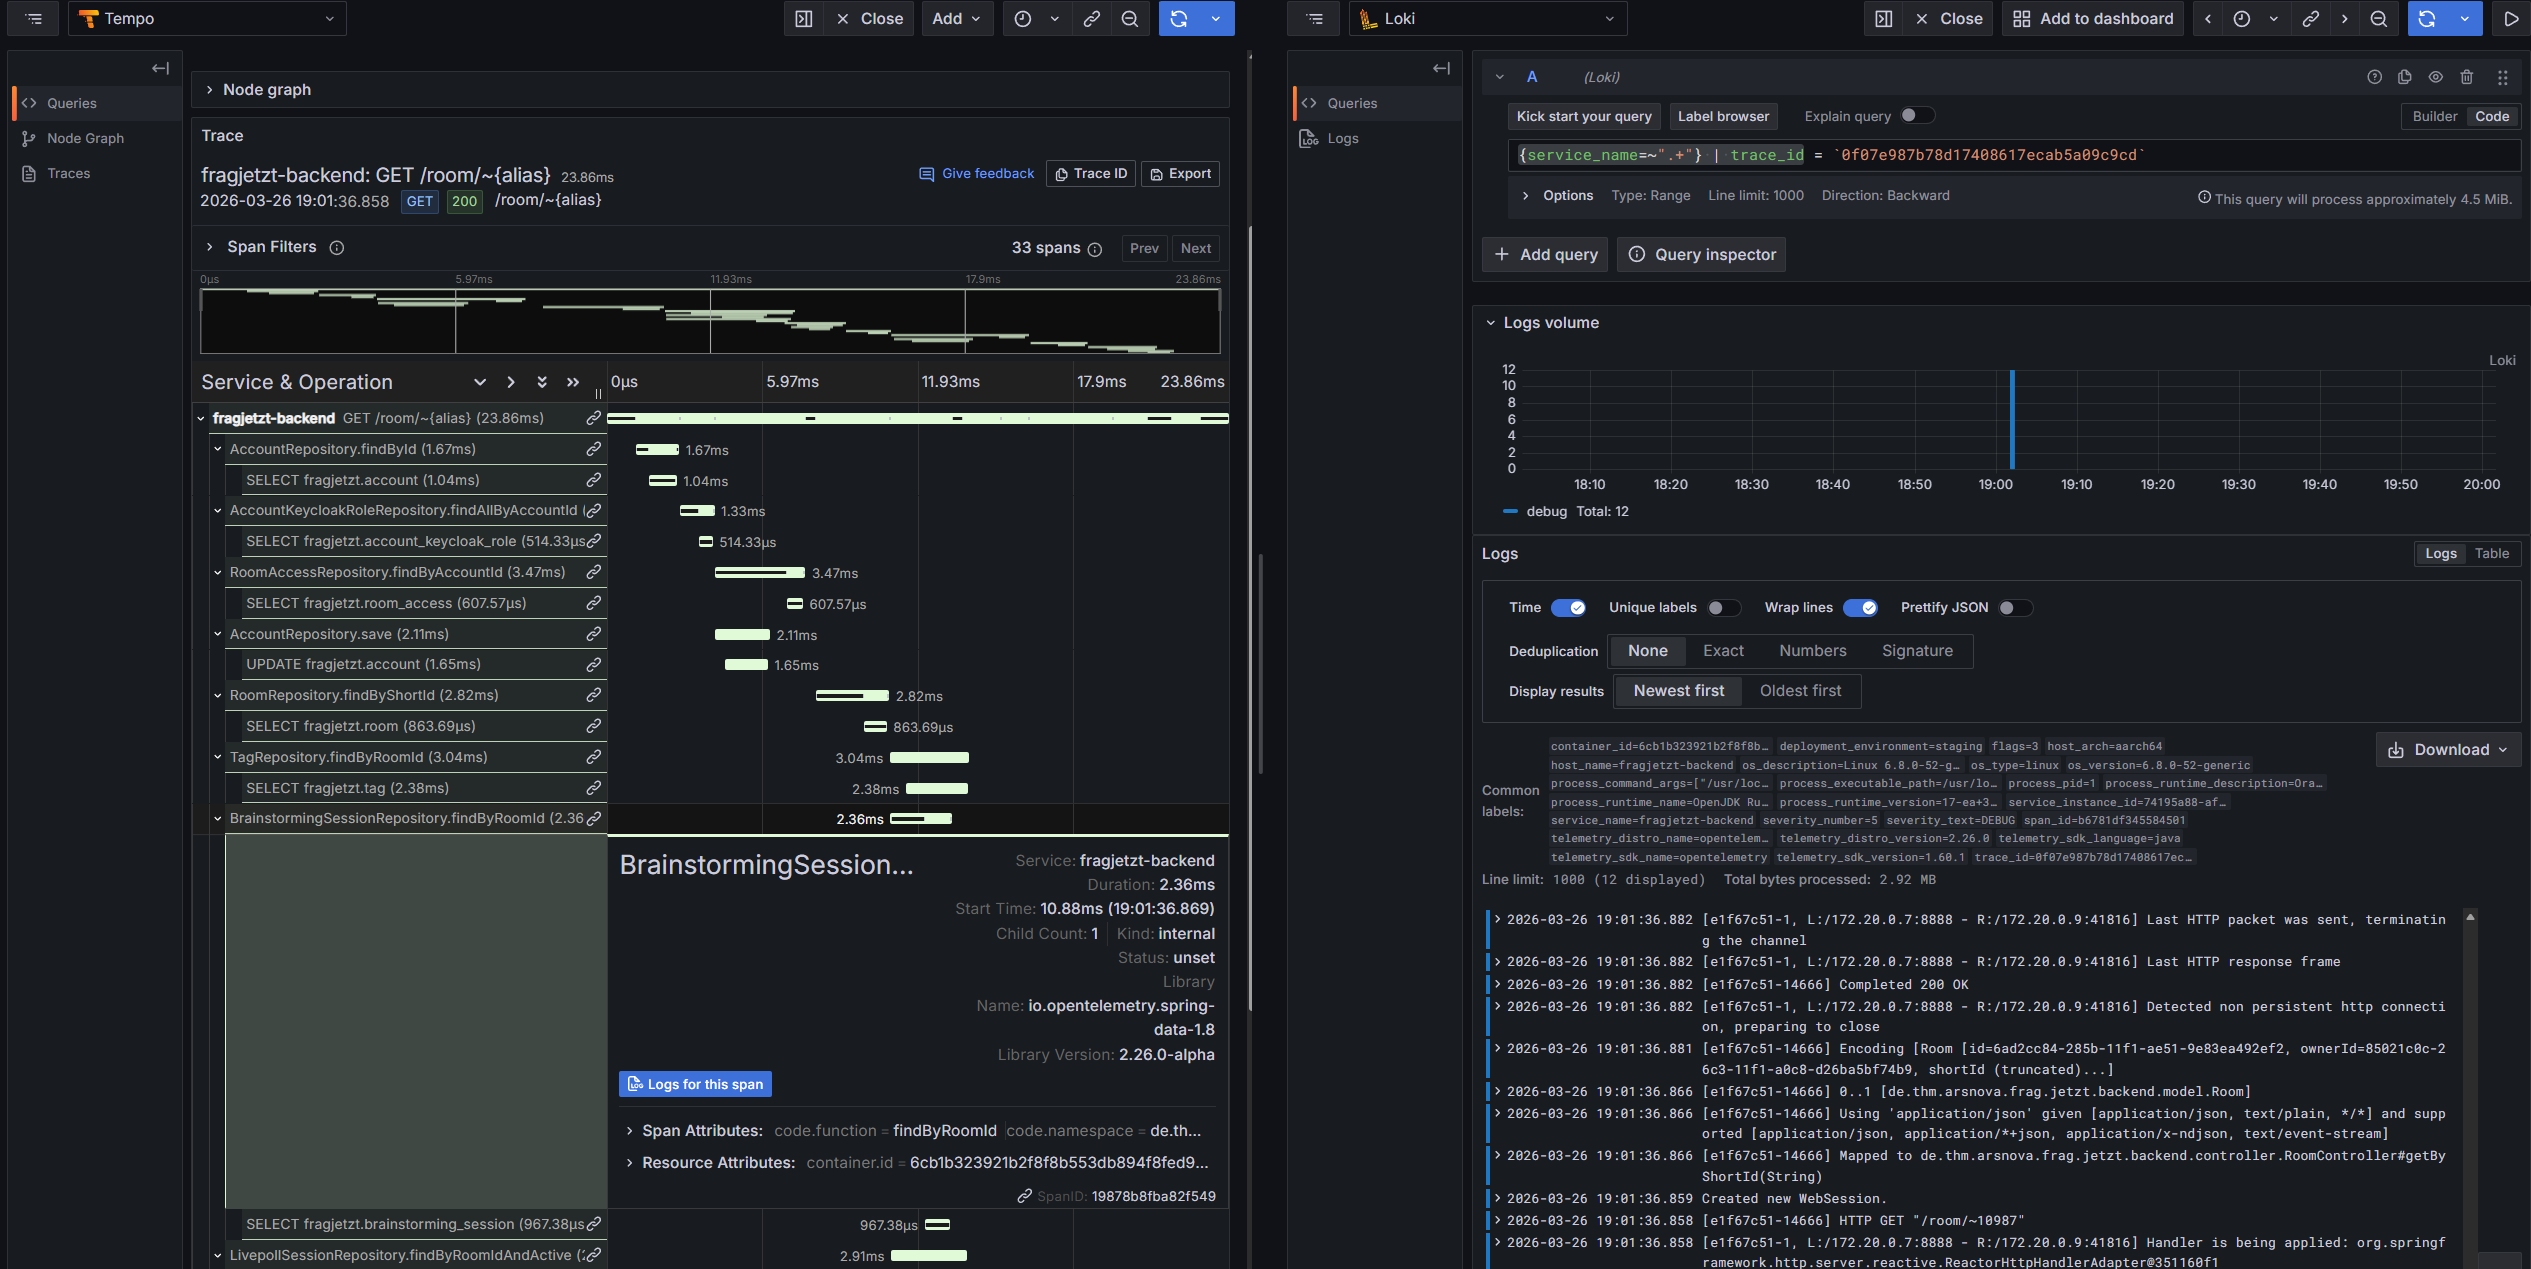
\includegraphics[width=\textwidth]{images/fig_trace_to_logs_correlation.png}
\caption[Trace-Waterfall in Tempo für den Endpunkt \texttt{GET /room/\{id\}/moderator} mit 11~Spans und zugeordneten Datenbankoperationen.]{Trace-Waterfall in Tempo für den Endpunkt \texttt{GET /room/\{id\}/moderator} mit 11~Spans und zugeordneten Datenbankoperationen. Der rechte Bereich zeigt die korrelierten Loki-Logs, erreichbar über die Funktion \emph{Logs for this span}. \small Quelle: Eigene Darstellung (Screenshot, Staging-Server).}
\label{fig:trace-waterfall}
\end{figure}

Die Nachvollziehbarkeit endet an den Grenzen der instrumentierten Komponenten. Der AI Provider und das Frontend sind nicht instrumentiert. Für den instrumentierten Backend-Pfad ist die Request-Rekonstruktion funktional gegeben, für das Gesamtsystem bleibt sie unvollständig. Der Erfüllungsgrad wird daher als \emph{teilweise erfüllt} bewertet.


\subsection{A2: Mehrstufige Messbarkeit entlang der Golden Signals}

\emph{Prüffrage: Deckt die Instrumentierung alle drei Messebenen ab?}

Das Golden-Signals-Dashboard bildet alle vier Dimensionen in separaten Sektionen ab. Im Belastungsszenario stieg die p95-Latenz unter CPU-Last von rund 20\,ms auf über 500\,ms, was im Dashboard sofort sichtbar wurde. Nach dem temporären Stopp der Datenbank stieg die 5xx-Rate und die betroffenen Endpunkte erschienen in der Fehlertabelle. Die drei Messebenen, Applikationsmetriken über den OTel Agent, Infrastrukturmetriken über Exporter und Trace-basierte Span-Metriken über Tempo, sind für die instrumentierten Dienste abgedeckt. Die Lücke betrifft die fehlende Frontend-Telemetrie. Der Erfüllungsgrad wird als \emph{weitgehend erfüllt} eingestuft.


\subsection{A3: Strukturiertes, korrelierbares Logging}

\emph{Prüffrage: Können Logeinträge über Korrelations-IDs verknüpft werden?}

Die bidirektionale Korrelation zwischen Logs und Traces konnte auf dem Staging-Server nachgewiesen werden. Von einem Trace in Tempo führt die Funktion \emph{Logs for this span} zu einer Loki-Abfrage, die nach Trace-ID und Dienstname filtert. In der Gegenrichtung enthält jeder Log-Eintrag in Loki ein klickbares \emph{TraceID}-Feld, das direkt zum zugehörigen Trace navigiert. Diese Verknüpfung wurde über ein Derived Field in der Loki-Datenquellenkonfiguration realisiert.

\begin{figure}[htb]
\centering
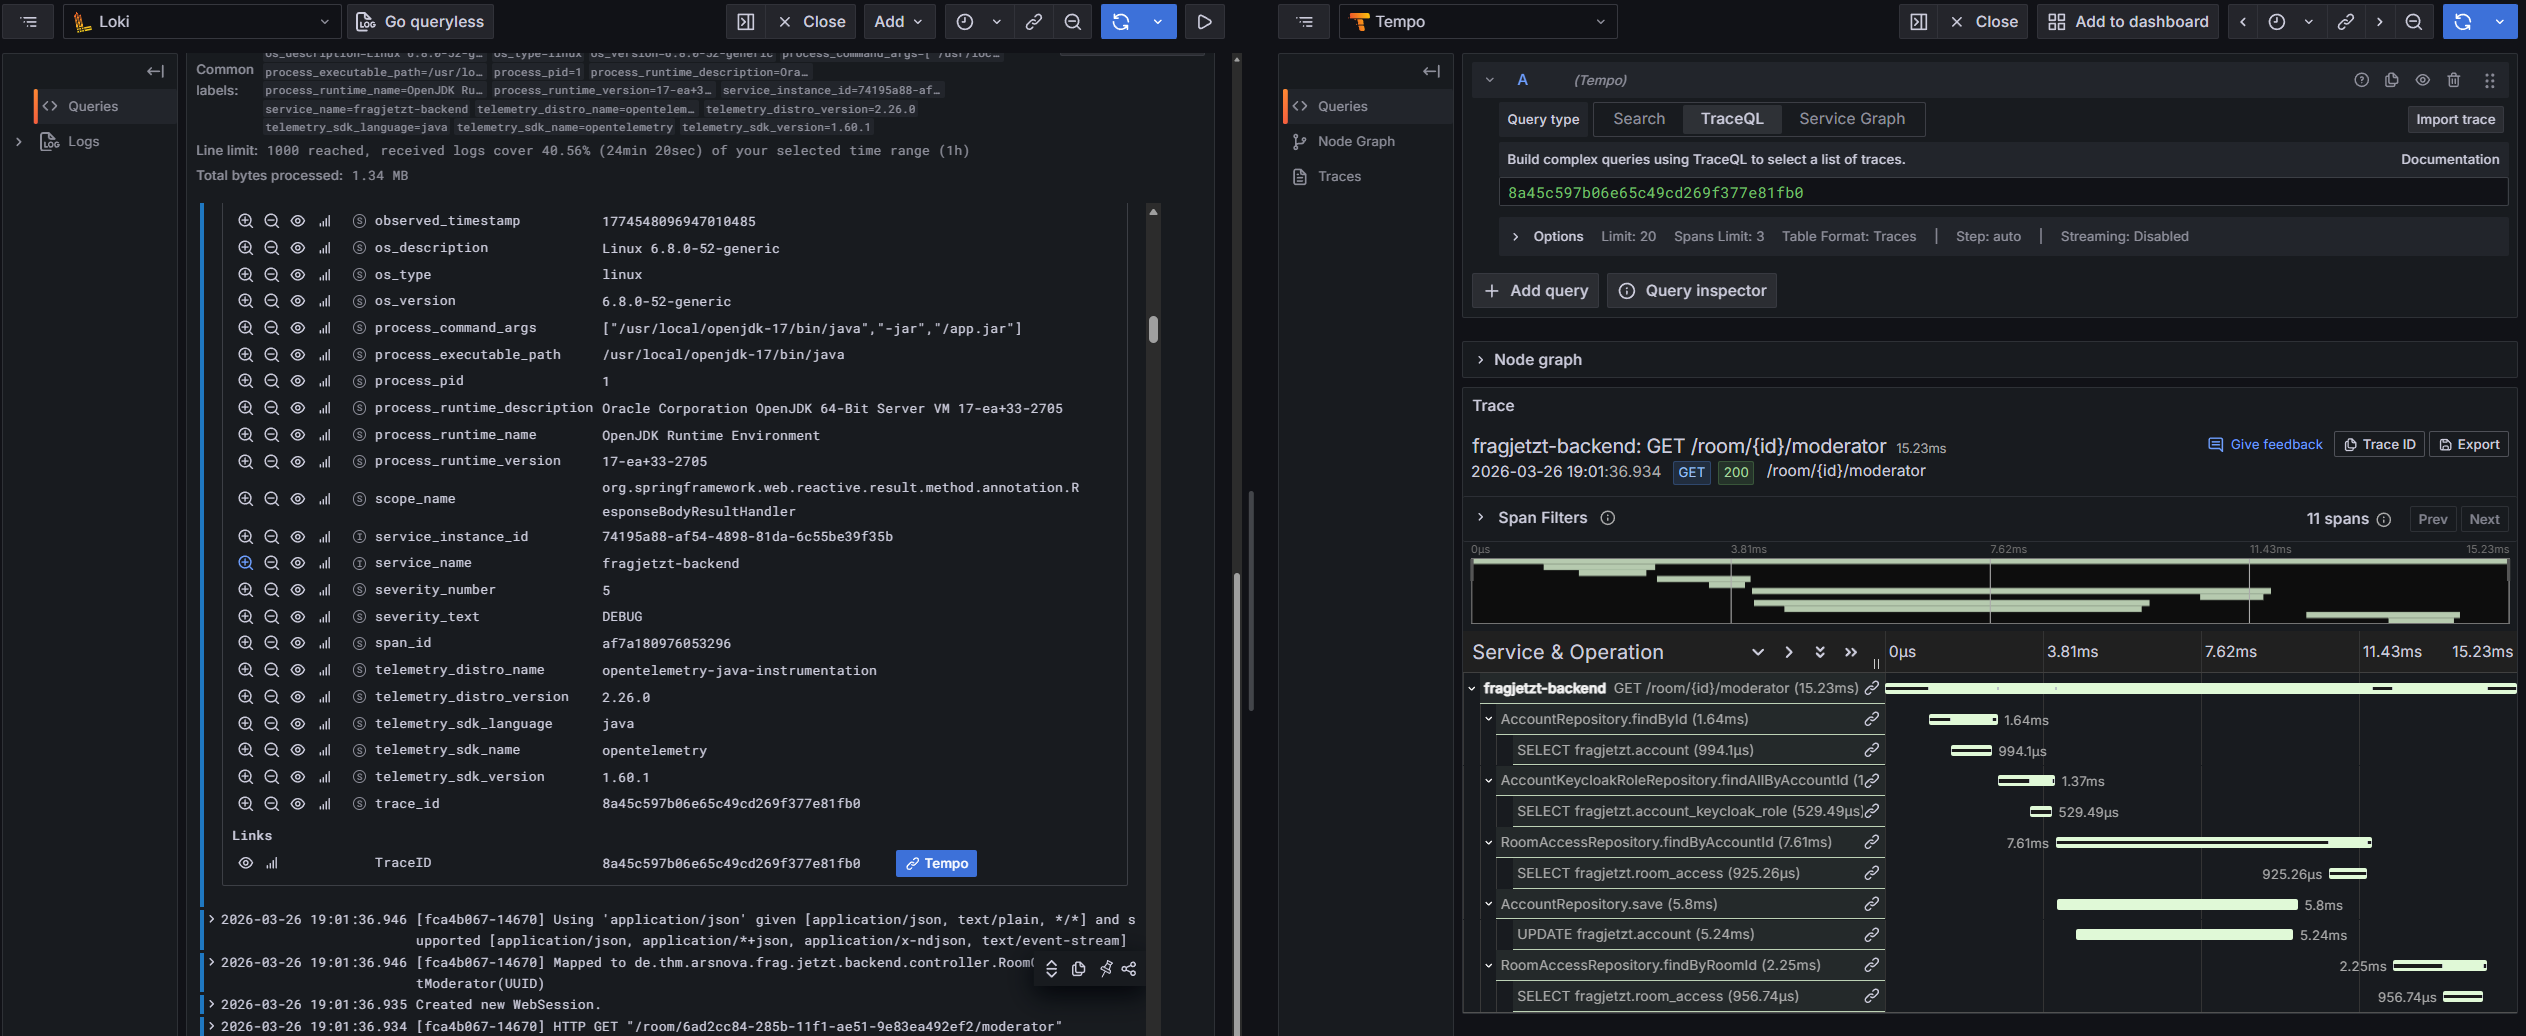
\includegraphics[width=\textwidth]{images/fig_log_to_trace_correlation.png}
\caption[Log-to-Trace-Korrelation in Loki: Ein Logeintrag mit klickbarem TraceID-Link (links) navigiert zum zugehörigen Trace-Waterfall in Tempo (rechts).]{Log-to-Trace-Korrelation in Loki: Ein Logeintrag mit klickbarem TraceID-Link (links) navigiert zum zugehörigen Trace-Waterfall in Tempo (rechts). \small Quelle: Eigene Darstellung (Screenshot, Staging-Server).}
\label{fig:log-to-trace}
\end{figure}

Da die Kernfunktion der Korrelierbarkeit nachgewiesen wurde, wird A3 als \emph{erfüllt} bewertet. Für den Produktivbetrieb wäre eine Reduktion auf strukturierte JSON-Protokollierung erforderlich.


\subsection{A4: Handlungsfähige Alarmierung}

\emph{Prüffrage: Reagieren Alarme auf nutzerwirksame Zustände und enthalten sie ausreichend Kontext für eine Erstreaktion?}

Der Latenz-Alert wurde durch künstlich erzeugten CPU-Druck auf den Backend-Container im Zustand \emph{Firing} ausgelöst. Abbildung~\ref{fig:alert-firing} zeigt den Alarm mit Symptombeschreibung, Prüfpfad und Runbook-Link in den Annotations. Die Multi-Signal-Logik bewährte sich: In Leerlaufphasen ohne aktive Requests verhinderte die Mindest-Traffic-Rate von 0,1\,req/s, dass der Alert fälschlicherweise auslöste.

\begin{figure}[htb]
\centering
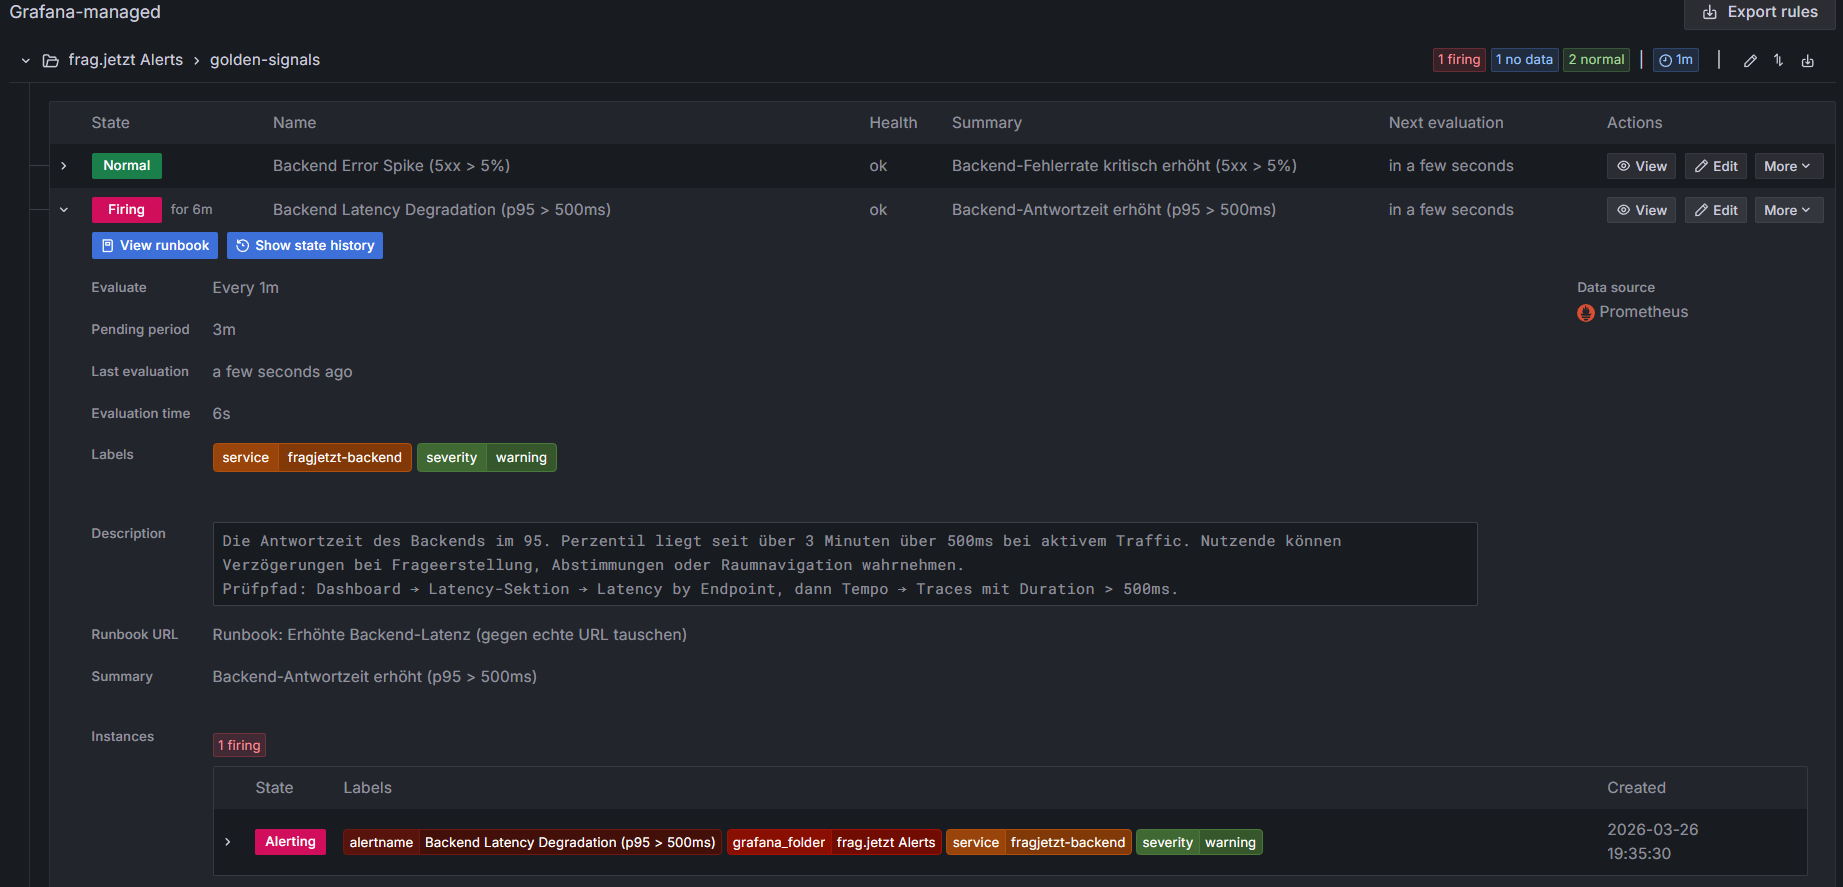
\includegraphics[width=\textwidth]{images/fig_firing_latency_alert.png}
\caption[Latenz-Alert im Zustand \emph{Firing} nach 6~Minuten. Die Annotations enthalten Symptombeschreibung, Prüfpfad und Runbook-Link.]{Latenz-Alert im Zustand \emph{Firing} nach 6~Minuten. Die Annotations enthalten Symptombeschreibung, Prüfpfad und Runbook-Link. \small Quelle: Eigene Darstellung (Screenshot, Staging-Server).}
\label{fig:alert-firing}
\end{figure}

Der Fehler-Alert konnte zuverlässig ausgelöst werden. Die Rate-Berechnung lieferte allerdings bei kurzen Betrachtungszeiträumen keine konsistenten Werte, vermutlich aufgrund einer Diskrepanz zwischen dem dynamisch berechneten Abfragefenster und der Erfassungssemantik der OTel-basierten Metriken. Der Sättigungs-Alert wurde nicht als eigenständiges Szenario getestet, die zugrunde liegende Metrik war jedoch korrekt verfügbar.

Für den Latenz-Alert ist die Alerting-Konzeption funktional validiert. Für den Fehler-Alert zeigt sich ein Datenqualitätsproblem in der kurzfristigen Metrikdarstellung, das die konzeptionelle Validität der Regel nicht infrage stellt, aber die operative Kurzfristdiagnose einschränkt. Der Erfüllungsgrad wird als \emph{teilweise erfüllt} eingestuft.


\subsection{A5: Beobachtbarkeit der Infrastrukturschicht}

\emph{Prüffrage: Werden Container-Ressourcen, Datenbankpool-Auslastung und Queue-Tiefen erfasst?}

Die Infrastruktur-Sektion des Dashboards beantwortet diese Frage positiv. Abbildung~\ref{fig:infrastructure-dashboard} zeigt PostgreSQL-Verbindungszähler, RabbitMQ-Queue-Tiefen, Host-Ressourcen und den Service Graph. Während der Belastungstests stieg die Zahl aktiver PostgreSQL-Verbindungen von einem Normalniveau um 3 auf temporär über 10. Alle fünf Infrastruktur-Exporter lieferten während des gesamten Evaluationszeitraums durchgängig Metriken. Da die Metriken verfügbar und plausibel sind, nicht aber alle Indikatoren unter gezielter Last geprüft wurden, wird A5 als \emph{weitgehend erfüllt} bewertet.

\begin{figure}[htb]
\centering
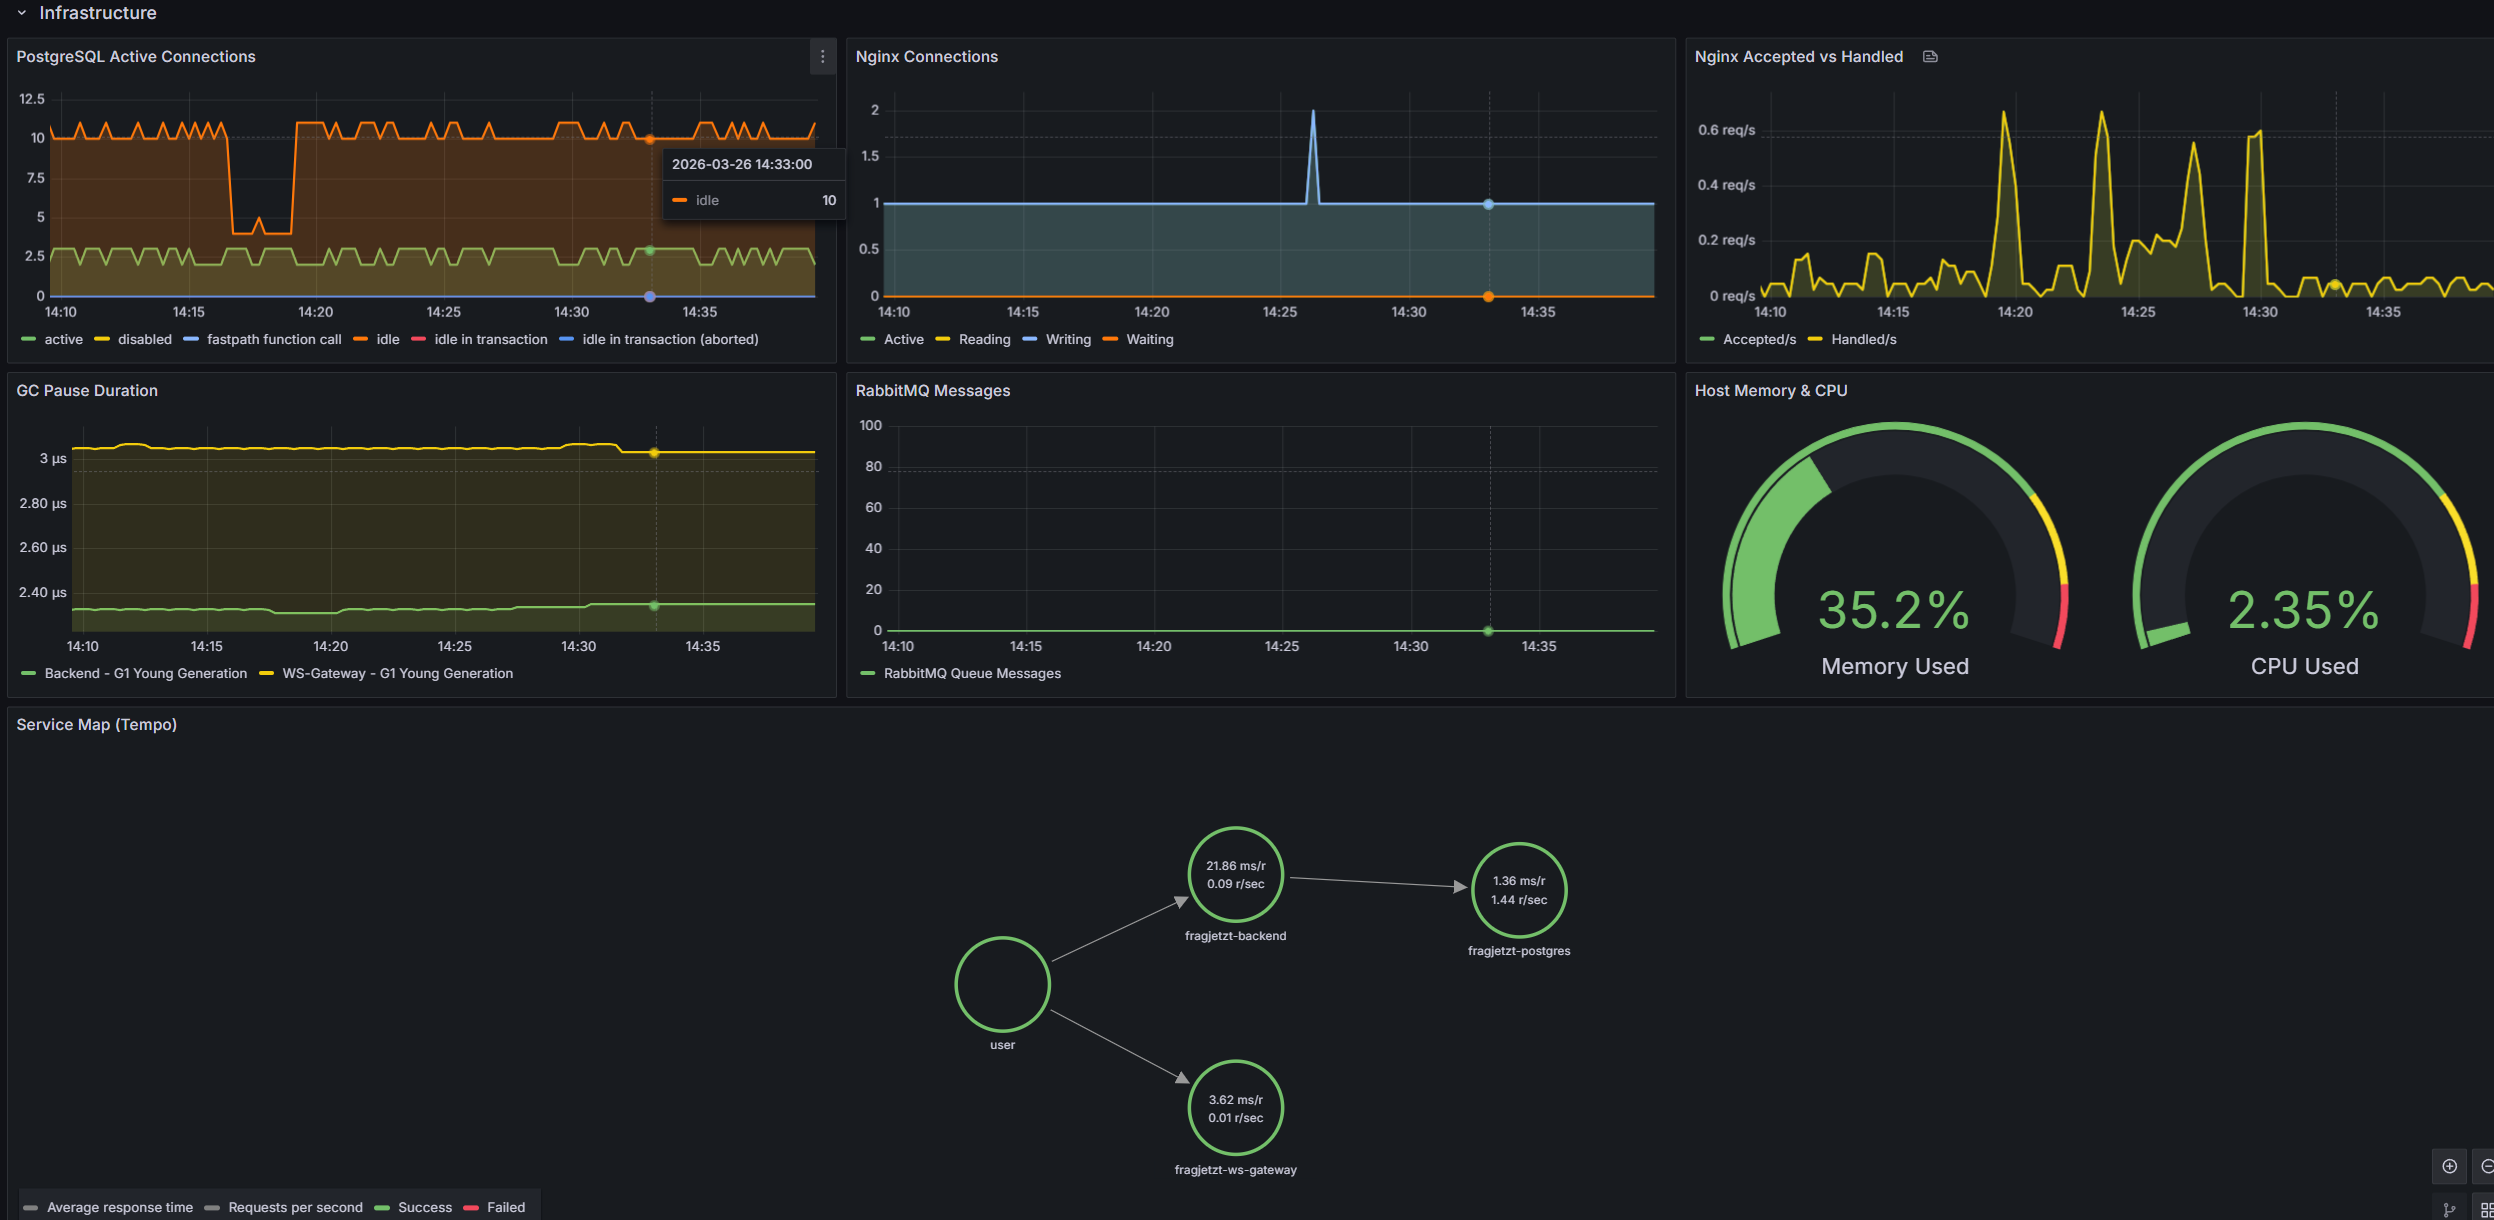
\includegraphics[width=\textwidth]{images/Grafana-Dashboard_Infrastructure.png}
\caption[Infrastruktur-Sektion des Golden-Signals-Dashboards mit PostgreSQL-Verbindungen, RabbitMQ-Queue-Tiefe, Host-Ressourcen und Service Graph.]{Infrastruktur-Sektion des Golden-Signals-Dashboards mit PostgreSQL-Verbindungen, RabbitMQ-Queue-Tiefe, Host-Ressourcen und Service Graph. \small Quelle: Eigene Darstellung (Screenshot, Staging-Server).}
\label{fig:infrastructure-dashboard}
\end{figure}


\section{Übergreifende Bewertungsdimensionen}

\paragraph{Stakeholder-Tauglichkeit.}
Für die DevOps-Perspektive ist der Prototyp funktional nutzbar: Dashboard, Alerting-Regeln und Runbooks liefern eine zusammenhängende Diagnoseinfrastruktur. Für die Entwicklungsperspektive ermöglicht Grafana Explore die direkte Abfrage von Traces, Logs und Metriken mit bidirektionaler Korrelation, ein dediziertes Entwickler-Dashboard wurde jedoch nicht umgesetzt. Für die Product-Owner-Perspektive fehlt im Prototyp eine eigene Sicht, die technisch aus den vorhandenen Datenquellen ableitbar wäre.

\paragraph{Abdeckung der Risikopunkte.}
Von den sechs identifizierten Risikopunkten werden R2 (DB-Contention), R3 (Intransparenz ohne Tracing) und R5 (Ressourcenverdrängung) durch den Prototyp direkt adressiert. R3 wurde durch die Einführung von Distributed Tracing beseitigt. R1 (fehlende Timeouts) und R4 (Backend als Single Point of Failure) bleiben als architektonische Defizite bestehen, die über Beobachtbarkeit sichtbar, aber nicht lösbar sind.

\paragraph{Umsetzungsrealismus.}
Die Gesamtdauer von der initialen Stack-Konfiguration bis zum funktionierenden Dashboard betrug wenige Arbeitstage. Der laufende Betrieb des Observability-Stacks erfordert allerdings ein eigenes Ressourcenbudget, das bei der Kapazitätsplanung des Hosts berücksichtigt werden muss.


\section{Grenzen und methodische Einschränkungen}

Die Evaluation unterliegt fünf Einschränkungen.

\emph{Erstens, unvollständige Dienstabdeckung.} Backend und WS-Gateway sind instrumentiert, AI Provider und Frontend nicht. Die Bewertung von A1 und A2 gilt nur für einen Teil des Gesamtsystems.

\emph{Zweitens, Stabilität des Observability-Stacks unter Last.} Tempo wurde während der Belastungstests durch Speichererschöpfung beendet (OOM-Kill), woraufhin auch der OTel Collector den Betrieb einstellte. Infrastrukturmetriken über die Prometheus-Exporter blieben unberührt. Der Vorfall verdeutlicht, dass der Observability-Stack selbst eine Fehlerquelle darstellt, deren Auswirkungen auf einem Single-Host-System die Beobachtbarkeit des Gesamtsystems beeinträchtigen.

\emph{Drittens, eingeschränkte Aussagekraft der Rate-Berechnung.} Die PromQL-Variable \texttt{\$\_\_rate\_interval} lieferte bei kurzen Betrachtungszeiträumen inkonsistente Ergebnisse für die HTTP-5xx-Rate. In längeren Zeitfenstern (ab circa 12~Stunden) waren die Werte korrekt. Diese Einschränkung betrifft die Dashboard-Darstellung, nicht die Alerting-Regeln mit festen Zeitfenstern.

\emph{Viertens, fehlende Produktivdaten.} Alle Tests wurden mit synthetischer Last durchgeführt. Reale Nutzungsmuster, insbesondere die Lastspitzen während Lehrveranstaltungen, konnten nicht abgebildet werden. Die Schwellenwerte müssten im Produktivbetrieb anhand realer Lastprofile kalibriert werden.

\emph{Fünftens, prototypische Testmethodik.} Die Belastungsszenarien wurden manuell über Konsolen-Schleifen und Container-Operationen durchgeführt. Für eine belastbarere Validierung wäre ein dedizierter HTTP-Lastgenerator mit kontrollierten Lastprofilen erforderlich.
% !TEX root = ../Thesis.tex

% =============================================================================
% KAPITEL 9 – Diskussion
% =============================================================================
 
\chapter{Diskussion}
 
Die Evaluation in Kapitel~8 hat die Ergebnisse der prototypischen Umsetzung an den Anforderungen aus Kapitel~3 gemessen und dabei sowohl funktionale Stärken als auch offene Lücken identifiziert. Das vorliegende Kapitel ordnet diese Befunde in den Kontext der wissenschaftlichen Literatur ein, bewertet die Übertragbarkeit auf vergleichbare Plattformen und grenzt den wissenschaftlichen vom praktischen Beitrag der Arbeit ab.
 
 
\section{Einordnung der Ergebnisse im Verhältnis zur Literatur}
 
Die Arbeit bestätigt mehrere Grundannahmen der Observability-Literatur auf konzeptioneller Ebene und konkretisiert sie zugleich um operative Erkenntnisse aus der prototypischen Umsetzung. Ein erheblicher Teil der herangezogenen Literatur behandelt Observability entweder auf konzeptioneller Ebene oder entlang konkreter Frameworks und Werkzeuge \parencite[S.~72034]{faseeha2025observability}, während die Integration heterogener Telemetriequellen und die Interoperabilität zwischen verschiedenen Werkzeugen als eigenständige Herausforderung beschrieben werden \parencite[S.~105]{sakinala2025observability}. Die vorliegende Arbeit ergänzt diese Perspektive um fallbezogene Befunde aus einer konkreten Implementierung.
 
Auf der Bestätigungsseite stehen drei Befunde. Erstens erweist sich die Kombination der drei Telemetriepfeiler Logs, Metriken und Traces als praktisch tragfähig. \textcite[S.~22]{albuquerque2025tracing} beschreiben \emph{Application Metrics} und \emph{Infrastructure Metrics} als komplementäre Entwurfsmuster, deren Zusammenspiel eine vollständige Sicht auf einen Dienst ermöglicht. Die vorliegende Arbeit stützt diesen Befund, indem sie zeigt, dass erst die Verknüpfung von Span-basierten Applikationsmetriken mit Exporter-basierten Infrastrukturmetriken in einem gemeinsamen Dashboard eine diagnostisch nutzbare Gesamtsicht erzeugt. Ohne diese Verknüpfung blieben die Infrastrukturindikatoren interpretationsarm, da sie zwar mögliche Engpässe anzeigen, nicht aber deren tatsächliche Ursache offenlegen \parencite[S.~20]{albuquerque2025tracing}.
 
Zweitens hat sich das Prinzip der symptomorientierten Alarmierung im Prototyp für den Latenz- und den Fehler-Alert bewährt, die jeweils nach einer Mehrsignal-Logik aufgebaut sind. Der Latenz-Alert verlangt neben der p95-Überschreitung gleichzeitig eine Mindest-Traffic-Rate als Vorbedingung und verhinderte in der Evaluation falsch-positive Auslösungen in Leerlaufphasen. Damit bestätigt die Arbeit die Empfehlung, Alarme auf nutzerseitig wahrnehmbare Zustände auszurichten und mehrere korrelierte Größen zu einem aussagekräftigeren Alarm zu kombinieren \parencite[S.~175]{vinnakota2025creating}. Einschränkend ist anzumerken, dass der Infrastruktur-Sättigungsalert in der prototypischen Regeldefinition vereinfacht umgesetzt wurde, sodass eine seiner Alternativbedingungen auch ohne gleichzeitige Servicewirkung feuern konnte. Die Mehrsignal-Logik ist dort konzeptionell angelegt, aber nicht durchgängig implementiert.
 
Drittens belegt die Arbeit, dass Auto-Instrumentierung über den OTel Java Agent einen niedrigschwelligen Einstieg in Distributed Tracing ermöglicht. \textcite[S.~52]{bissig2024unified} stellen fest, dass der mentale Aufwand für Auto-Instrumentierung in synthetischen Benchmarks gering ausfällt. Für frag.jetzt bestätigt sich dieser Befund insofern, als die Instrumentierung des Spring-Boot-Backends ohne Codeänderungen funktionierte und unmittelbar verwertbare Traces erzeugte.
 
Neben diesen Bestätigungen macht die Arbeit drei Aspekte sichtbar, die in der Literatur eher abstrakt behandelt werden und für den Fall frag.jetzt konkrete Gestalt annehmen. Der erste betrifft die operative Komplexität. Die Literatur beschreibt überwiegend konzeptionelle Modelle und empfohlene Vorgehensweisen. Die prototypische Umsetzung zeigt für den Fall frag.jetzt, dass infrastrukturelle und konfigurationsbezogene Herausforderungen einen erheblichen Einfluss auf die tatsächliche Nutzbarkeit eines Observability-Systems haben. Der OOM-Kill von Tempo, die Netzwerkprobleme in der Docker-Compose-Topologie und das Span-Rauschen durch die Auto-Instrumentierung traten als konkrete Problemkategorien auf, die in den herangezogenen Quellen nicht in dieser Spezifik behandelt werden. \textcite[S.~9]{Niedermaier2019onObservability} identifizieren zwar knappe Ressourcen und reaktive Implementierung als typische Herausforderungen (C7, C9), verbleiben aber auf einer übergeordneten Ebene. Die Kaskadeneffekte, die auf einem Single-Host-System durch den Observability-Stack selbst entstehen können, werden dort nicht adressiert.
 
Der zweite Aspekt betrifft die Signalqualität. Die Literatur diskutiert Sampling als Strategie zur Volumenreduktion \parencite[S.~10]{albuquerque2025tracing}. Die vorliegende Arbeit konkretisiert diesen Punkt, indem sie gezieltes Filtering auf Collector-Ebene einsetzt, das diagnostisch wertlose Spans verwirft, bevor sie gespeichert werden. Im Unterschied zum Sampling, das relevante Daten anteilig verlieren kann, erlaubt das Filtering eine inhaltlich begründete Selektion. Dieser Ansatz adressiert ein Problem, das \textcite[S.~52]{bissig2024unified} für reale Projekte unter dem Stichwort unerwarteten Verhaltens der Instrumentierung beschreiben, ohne eine Lösungsstrategie auf Collector-Ebene vorzuschlagen.
 
Der dritte Aspekt betrifft die Validierbarkeit von Alerting-Regeln. \textcite[S.~175--176]{vinnakota2025creating} fordern ausdrücklich, Alarme vor dem produktiven Einsatz rigoros zu testen, etwa durch synthetisches Monitoring, Fehlerinjektion und kontrollierte Störungssimulationen in Staging-Umgebungen. Die Evaluation zeigt exemplarisch, dass diese Forderung in der Praxis auf erhebliche Reibung stoßen kann. Der Fehler-Alert ließ sich definieren und konfigurieren, aber nicht zuverlässig zum Feuern bringen, weil die Interaktion zwischen dynamischem Abfragefenster, PromQL-Aggregationslogik und der Erfassungssemantik der OTel-Metriken ein eigenständiges technisches Problem darstellt. Die Literatur benennt die Notwendigkeit des Testens, beleuchtet jedoch die konkreten Schwierigkeiten, die sich aus dem Zusammenspiel von Metriksemantik, Query-Verhalten und Staging-Verifikation ergeben, nur begrenzt.
 
 
\section{Übertragbarkeit auf ähnliche cloud-native Plattformen}
 
Die Frage der Übertragbarkeit lässt sich in drei Stufen beantworten, die den Grad der Kontextabhängigkeit widerspiegeln.
 
\emph{Hoch übertragbar} sind drei methodische Elemente, die unabhängig von der spezifischen Architektur von frag.jetzt funktionieren. Die \emph{Signal-Matrix-Methodik} aus Kapitel~6.4, die für jeden Dienst systematisch die vier Golden Signals auf konkrete Messgrößen, Zwecke und Stakeholder-Rollen abbildet, ist als Strukturierungswerkzeug auf jedes verteilte System anwendbar. Sie setzt lediglich voraus, dass die beteiligten Dienste und ihre kritischen Interaktionen bekannt sind. Die \emph{Fünf-Felder-Runbook-Struktur} (Symptom, Kontext, Diagnose, Behebung, Eskalation) ist ebenfalls stackunabhängig und lässt sich auf beliebige Alerting-Systeme anwenden. Die \emph{symptomorientierte Alert-Logik}, die nutzerwirksame Zustände als Auslöser verwendet und interne Ursachenindikatoren als Debugging-Kontext reserviert, folgt einem Prinzip, das in der SRE-Literatur als stackübergreifend gültig beschrieben wird \parencite[Kap.~\emph{Symptoms Versus Causes}]{ewaschukMonitoringDistributedSystems}.
 
\emph{Bedingt übertragbar} ist der OTel-Agent-basierte Instrumentierungsansatz. Der OTel Java Agent funktioniert besonders reibungsarm in JVM-basierten Umgebungen. Für Anwendungen in anderen Laufzeitumgebungen, etwa Python oder Node.js, kann der Aufwand höher ausfallen und zusätzliche manuelle Anpassungen erfordern \parencite[S.~52]{bissig2024unified}. Das Grundprinzip, die Instrumentierung über einen herstellerneutralen Standard zu entkoppeln und dadurch die Bindung an ein bestimmtes Backend zu vermeiden, bleibt jedoch unabhängig von der Laufzeitumgebung gültig. \textcite[S.~72034--72035]{faseeha2025observability} bestätigen, dass die Interoperabilität zwischen heterogenen Plattformen eine der zentralen offenen Herausforderungen darstellt, die durch standardisierte Telemetrieformate wie OpenTelemetry adressiert wird.
 
\emph{Kontextabhängig} sind die konkreten Implementierungsentscheidungen. Der LGTM-Stack hat sich für das Single-Host-Szenario von frag.jetzt als geeignet erwiesen, stellt aber keine universelle Empfehlung dar. Für Organisationen mit Kubernetes-nativer Infrastruktur und höherem Telemetrievolumen kommen andere Stack-Kombinationen oder skalierbare Varianten infrage \parencite[S.~498]{gudimetla2025transitioning}. Die Docker-Compose-Topologie und die konkreten Schwellenwerte der Alerting-Regeln sind systemspezifisch. Schwellenwerte müssen aus den jeweiligen Lastprofilen und nichtfunktionalen Anforderungen des Zielsystems abgeleitet werden, wie bereits in Kapitel~4.2 als methodischer Grundsatz formuliert.
 
Zusammengefasst sind die methodischen Konzepte, also das \emph{Wie} der Ableitung, die strukturierende Matrix und die Alert-Logik, übertragbar. Die konkreten technischen Entscheidungen, also das \emph{Womit} und die spezifischen Grenzwerte, bleiben kontextgebunden.
 
 
\section{Wissenschaftlicher und praktischer Beitrag}
 
Die Arbeit entwickelt kein neues theoretisches Modell für Observability. Ihr Beitrag liegt in der methodisch fundierten Anwendung, Integration und Operationalisierung bestehender Konzepte für einen konkreten Anwendungskontext.
 
Der \emph{wissenschaftliche Beitrag} besteht in der methodisch transparenten Ableitungslogik, die von der Systemanalyse über die Anforderungsdefinition und die servicebezogene Operationalisierung der Golden Signals bis zur kriteriengestützten Evaluation reicht. Dieses Vorgehen verbindet mehrere in der Literatur häufig getrennt behandelte Konzepte zu einem integrierten Strategieentwurf. Dazu gehören die Golden Signals als Strukturierungsheuristik, das Design komplementärer Metrikebenen, die symptomorientierte Alarmierung und die rollenbasierte Informationsaufbereitung. Die explizite Rückbindung an Prüffragen und Erfüllungsgrade in der Evaluation stellt sicher, dass die Ergebnisse nachvollziehbar und an den Anforderungen messbar bleiben. Darüber hinaus liefert die Arbeit fallbezogene operative Hinweise auf Problemkategorien, etwa Ressourcenkonflikte des Observability-Stacks mit der beobachteten Anwendung, die in der vorwiegend konzeptionell argumentierenden Literatur bislang wenig Raum einnehmen.
 
Der \emph{praktische Beitrag} umfasst eine funktionsfähige Observability-Infrastruktur für frag.jetzt, die aus Instrumentierungskonfigurationen, Dashboard-Definitionen, Alerting-Regeln und Runbooks besteht. Die dokumentierten Herausforderungen bei Netzwerktopologie, Ressourcendimensionierung und Signalfilterung sind für Teams, die Observability erstmals in einer Docker-Compose-basierten Umgebung einführen, unmittelbar verwertbar. Die Signal-Matrix und die Runbook-Struktur stehen als wiederverwendbare Artefakte zur Verfügung, die auch ohne den spezifischen Technologie-Stack adaptiert werden können.
 
Beide Beitragsebenen stehen in einem komplementären Verhältnis: Die methodische Ableitung gibt dem Prototyp seine wissenschaftliche Nachvollziehbarkeit, und der Prototyp gibt den methodischen Konzepten ihre praktische Überprüfbarkeit.
% =============================================================================
% KAPITEL 10 – Fazit und Ausblick (überarbeitet)
% =============================================================================
 
\chapter{Fazit und Ausblick}
 
Die vorliegende Arbeit ging von einem konkreten betrieblichen Defizit aus: Die Plattform frag.jetzt verfügte über eine funktionsfähige Deployment-Infrastruktur, erhob jedoch weder Metriken noch Traces noch korrelierbare Logs. Störungen wurden erst sichtbar, wenn Endnutzende bereits betroffen waren. Um dieses Defizit zu adressieren, wurde eine Observability-Strategie entwickelt, die von der Systemanalyse über die servicebezogene Operationalisierung der Four Golden Signals und die kriteriengestützte Stack-Auswahl bis zur prototypischen Umsetzung und Evaluation reicht. Die folgenden Abschnitte beantworten die drei Forschungsfragen, verdichten die wesentlichen Erkenntnisse und skizzieren priorisierte Anknüpfungspunkte für die Weiterentwicklung.
 
 
\section{Beantwortung der Forschungsfragen}
 
\textbf{FF1: Wie lassen sich die Four Golden Signals für die spezifischen Services (PWA-Frontend, Spring-Boot-Backend, PostgreSQL, KI-Services) von frag.jetzt konkret definieren und instrumentieren?}
 
Die Arbeit beantwortet diese Frage durch eine fünfstufige Ableitungslogik, die für jeden Dienst funktionale Rolle, kritische Interaktionen, geeignete Messgrößen, initiale Schwellenwerte sowie Visualisierungs- und Alarmierungskonsequenzen bestimmt. Das Ergebnis ist eine serviceübergreifende Signal-Matrix, die jedem Dienst pro Golden Signal eine primäre Messgröße, einen Erhebungszweck und eine Stakeholder-Zuordnung zuweist. Für die JVM-basierten Dienste ließ sich diese Ableitung über die Auto-Instrumentierung des OpenTelemetry Java Agent in eine funktionsfähige Telemetrie-Pipeline überführen, die HTTP-Spans, Datenbankoperationen und JVM-Metriken ohne Codeänderungen erfasst. Die Ableitung ist damit methodisch vollständig, praktisch jedoch bisher nur für einen Teil des Gesamtsystems nachgewiesen. Für den AI Provider und das Frontend steht die Instrumentierung noch aus.
 
\bigskip
 
\textbf{FF2: Welche Observability-Stack-Kombination erfüllt die Anforderungen von frag.jetzt unter Berücksichtigung der Single-Host-Topologie und der begrenzten Teamressourcen am besten?}
 
Der kriteriengestützte Vergleich dreier Architekturkandidaten ergab den LGTM-Stack aus Prometheus, Loki, Tempo und Grafana als geeignetste Lösung. Drei Argumente waren ausschlaggebend: der geringere Integrationsaufwand gegenüber Elastic Observability, die enge bidirektionale Korrelation zwischen Metriken, Traces und Logs innerhalb einer einzigen Oberfläche sowie die Austauschbarkeit einzelner Backend-Komponenten bei stabilem Instrumentierungskern über OpenTelemetry. Die prototypische Umsetzung auf dem Staging-Server bestätigte die Praktikabilität dieser Wahl, machte aber auch Ressourcenkonflikte sichtbar, die auf einem Single-Host-System besondere Aufmerksamkeit erfordern.
 
\bigskip
 
\textbf{FF3: Wie kann ein intelligentes Alerting-System konzipiert werden, das False Positives reduziert und actionable Insights für verschiedene Stakeholder-Rollen (DevOps, Entwickler, Product Owner) bereitstellt?}
 
Das entwickelte Alerting-Framework verfolgt zwei Prinzipien: symptomorientierte Auslösung, bei der Alarme an nutzerwirksame Zustände gekoppelt werden, und Multi-Signal-Logik, bei der ein primäres Fehlersignal erst in Kombination mit einer Mindest-Traffic-Rate als handlungsrelevant gewertet wird. Drei exemplarische Regeln wurden konfiguriert und mit strukturierten Runbooks in einer Fünf-Felder-Struktur verknüpft. Alle drei Alerts konnten in der Evaluation durch gezielte Belastungsszenarien ausgelöst werden. In Leerlaufphasen ohne aktive Anfragen verhinderte die Traffic-Bedingung eine falsch-positive Auslösung, unter künstlicher CPU-Last feuerte der Latenz-Alarm korrekt. Der Sättigungs-Alert wurde durch Erschöpfung des PostgreSQL-Verbindungspools mit angepasstem Schwellenwert validiert und bestätigte die AND-Logik über die gesamte Debounce-Dauer. Für den Fehler-Alert zeigte sich ein Datenqualitätsproblem bei kurzfristigen Rate-Berechnungen, das die konzeptionelle Validität nicht infrage stellt. Das Konzept ist damit funktional abgesichert, bedarf aber für den Produktivbetrieb einer Kalibrierung der Schwellenwerte anhand realer Lastprofile.
  
Zusammenfassend lässt sich festhalten, dass das betriebliche Ausgangsdefizit nicht vollständig beseitigt, aber substanziell verkleinert wurde. frag.jetzt ist von einem weitgehend intransparenten Produktionsbetrieb ohne jegliche Telemetrie zu einer teilweise validierten, methodisch fundierten Observability-Basis überführt worden. Von den fünf Anforderungen aus Kapitel~3 wurden A3 (korrelierbare Logs) als erfüllt und A2 (mehrstufige Messbarkeit), A4 (handlungsfähige Alarmierung) sowie A5 (Infrastrukturbeobachtbarkeit) als weitgehend erfüllt bewertet. A1 (Ende-zu-Ende-Nachvollziehbarkeit) erreichte als einziges den Grad \emph{teilweise erfüllt}, weil die Instrumentierungsabdeckung unvollständig blieb. Die verbleibenden Lücken sind identifiziert und adressierbar, ohne die grundlegende Architektur verändern zu müssen.
 
 
\section{Zentrale Erkenntnisse und übertragbare Artefakte}
 
Über die Beantwortung der Forschungsfragen hinaus lassen sich drei übergreifende Erkenntnisse festhalten, die auch für vergleichbare Projekte von Bedeutung sind.
 
Die erste betrifft die operative Komplexität einer Observability-Einführung. Die prototypische Umsetzung zeigte, dass die eigentlichen Engpässe weniger in der konzeptionellen Ableitung von Messgrößen liegen als in deren technischer Realisierung. Speichererschöpfung bei Tempo, Netzwerktrennung zwischen Docker-Compose-Projekten und diagnostisch wertloses Span-Rauschen durch Auto-Instrumentierung traten als wiederkehrende Problemkategorien auf. Diese operativen Hürden werden in der herangezogenen Literatur eher abstrakt behandelt \parencite[S.~7--9]{Niedermaier2019onObservability}, erwiesen sich im vorliegenden Prototyp jedoch als die bestimmenden Faktoren für den Implementierungsaufwand. Insbesondere der OOM-Kill von Tempo verdeutlichte, dass die Beobachtungsinfrastruktur selbst zur Fehlerquelle werden kann, wenn ihre Ressourcendimensionierung nicht sorgfältig auf die verfügbaren Host-Kapazitäten abgestimmt ist \parencite[S.~52]{bissig2024unified}.
 
Die zweite Erkenntnis betrifft die praktische Einstiegshürde. Die Auto-Instrumentierung über den OpenTelemetry Java Agent ermöglichte die Erfassung von HTTP-Spans, Datenbankoperationen und JVM-Metriken ohne Codeänderungen an der Anwendung. Für ein Projekt, das Observability erstmals einführt und über begrenzte Teamressourcen verfügt, senkt dieser Ansatz den initialen Aufwand erheblich. Zugleich erfordert die resultierende Signalflut eine bewusste Qualitätssicherung. Statt stochastischem Samplings, das relevante Traces anteilig verlieren kann, erwies sich im vorliegenden Prototyp ein inhaltlich begründetes Filtering auf Collector-Ebene als zweckmäßig: Periodische Hintergrundprozesse ohne diagnostischen Wert wurden gezielt verworfen, sodass die verbleibenden Traces eine höhere Aussagekraft besaßen.
 
Die dritte Erkenntnis betrifft den eigentlichen Mehrwert der Arbeit über den Einzelfall hinaus. Drei Artefakte sind als methodische Bausteine auch auf vergleichbare cloud-native Plattformen übertragbar: die Signal-Matrix-Methodik, die für jeden Dienst die vier Golden Signals auf konkrete Messgrößen, Erhebungszwecke und Stakeholder-Rollen abbildet, die symptomorientierte Multi-Signal-Alert-Logik, die nutzerwirksame Zustände als Auslöser mit einer Traffic-Vorbedingung verknüpft, und die Fünf-Felder-Runbook-Struktur, die jeden Alarm mit Symptom, Kontext, Diagnoseschritten, Erstmaßnahmen und Eskalationspfad verbindet. Diese Artefakte sind unabhängig vom konkreten Technologie-Stack einsetzbar.
 
 
\section{Ausblick}
 
Die prototypische Umsetzung hat eine funktionsfähige Grundlage geschaffen, deren Weiterentwicklung sich nach Dringlichkeit und Nähe zu den beobachteten Einschränkungen priorisieren lässt.
 
Den unmittelbar nächsten Schritt bildet die Validierung unter produktionsnahen Bedingungen. Die Belastungsszenarien in Kapitel~8 wurden manuell über Konsolen-Schleifen durchgeführt und bilden reale Nutzungsmuster nur eingeschränkt ab. Ein dedizierter HTTP-Lastgenerator mit kontrollierten Lastprofilen, ergänzt um gezielte Fault-Injection-Szenarien, würde die Aussagekraft der Alerting-Regeln und Schwellenwerte erheblich stärken. Auch das in der Evaluation beobachtete Datenqualitätsproblem bei kurzfristigen Rate-Berechnungen ließe sich unter systematischeren Testbedingungen gezielter eingrenzen.
 
Der zweite Schritt betrifft die Erweiterung der Instrumentierungsabdeckung. Der AI Provider ist als Python-basierter Dienst mit FastAPI nicht durch den Java Agent abgedeckt und müsste über das OpenTelemetry Python SDK instrumentiert werden. Ebenso fehlt eine Browser-Telemetrie für das Angular-Frontend. Erst mit diesen Erweiterungen ließe sich die Ende-zu-Ende-Nachvollziehbarkeit (A1) vollständig realisieren und die in Kapitel~6 konzipierte Signal-Matrix auch für die bisher nicht instrumentierten Dienste praktisch einlösen.
 
Drittens steht die Ableitung formaler Service Level Objectives aus. Die Arbeit hat SLOs bewusst ausgeklammert, weil für frag.jetzt keine historischen Produktivdaten vorliegen. Sobald die Instrumentierung im Produktivbetrieb aktive Lastprofile erfasst, können aus den erhobenen Metriken SLIs abgeleitet und mit Zielwerten hinterlegt werden. Dieser Schritt würde das regelbasierte Alerting um eine geschäftsbezogene Steuerungsebene erweitern \parencite[S.~11--12]{Niedermaier2019onObservability}.
 
Viertens hat die prototypische Umsetzung gezeigt, dass die Ressourcendimensionierung des Observability-Stacks auf einem Single-Host-System sorgfältiger Abstimmung bedarf. Eine systematische Ermittlung von Mindest-, Durchschnitts- und Maximalverbräuchen der einzelnen Observability-Container unter verschiedenen Lastszenarien würde die Grundlage für belastbare Speicherlimits schaffen und das Risiko von OOM-Kills reduzieren.
 
Fünftens fehlt im Prototyp die in Kapitel~6 konzipierte rollenspezifische Dashboard-Sicht für den Product Owner. Die Evaluation hat gezeigt, dass die DevOps-Perspektive funktional nutzbar und die Entwicklungsperspektive über Grafana Explore adressierbar ist. Für die Product-Owner-Perspektive, die verdichtete Indikatoren wie aktive Raumsitzungen und globale Fehlerraten zeigen könnte, wäre ein eigenes Dashboard aus den vorhandenen Datenquellen ableitbar und würde die Stakeholder-Tauglichkeit der Strategie vervollständigen.
 
Langfristig könnte das regelbasierte Alerting um anomaliebasierte Verfahren ergänzt werden \parencite[S.~40]{mistry2025future}. Statische Schwellenwerte bilden saisonale Lastschwankungen nur unzureichend ab \parencite[S.~174]{vinnakota2025creating}. Ansätze, die aus historischen Metriken dynamische Baselines ableiten, könnten die Erkennungsrate verbessern und die Anzahl falsch-positiver Alarme weiter senken \parencite[S.~75]{alsubaie2025exploring}. Eine solche Erweiterung setzt allerdings einen ausreichenden Bestand an historischen Telemetriedaten voraus \parencite[S.~273]{abieba2025advanced} und wäre als spätere Ausbaustufe zu betrachten. Vorrangig ist für frag.jetzt daher nicht eine weitere funktionale Ausweitung, sondern zunächst die Konsolidierung, Vervollständigung und empirische Absicherung der entwickelten Observability-Basis.
 
\newpage
\printbibliography[heading=bibintoc, title=Literaturverzeichnis]%
 
\clearpage
\phantomsection
\addcontentsline{toc}{chapter}{Index}
\printindex
\IfDefined{printnomenclature}{\printnomenclature{}}
 
\appendix
% !TEX root = ../Thesis.tex

\chapter{Verzeichnis der KI-Nutzung}
\label{ch:ki-nutzung}

\input{content/00_KIErklaerung}

Tabelle~\ref{tab:ki-nutzung} listet alle in dieser Arbeit verwendeten KI-Werkzeuge auf.
\newpage


\section{Copilot Prompts für die unterstützende Systemanalyse von frag.jetzt}
\label{sec:anhang-copilot-prompts}

\begin{lstlisting}[caption={Copilot-Prompts zur Architekturanalyse}]
Analysiere die Projektstruktur von frag.jetzt. Welche Module, Services und Hauptkomponenten gibt es? Erstelle eine tabellarische Uebersicht mit Modulname, Technologie/Framework und Hauptverantwortung.
Identifiziere alle externen HTTP-Aufrufe (REST-Clients, WebClients, Feign-Clients) im Spring-Boot-Backend. Welche externen Dienste werden aufgerufen, mit welchen Endpunkten, und gibt es Timeout- oder Retry-Konfigurationen?
Liste alle REST-Controller im Backend auf. Gruppiere sie nach fachlicher Funktion (z. B. Room-Management, Question-Management, Auth, AI-Service) und notiere die HTTP-Methoden und Pfade.
Gibt es bereits Observability-bezogene Konfigurationen? Suche nach: Micrometer, Actuator, OpenTelemetry, Prometheus, Logging-Frameworks (Logback, Log4j), Health-Check-Endpoints, Tracing-Bibliotheken.
Analysiere die Datenbankschicht. Welche Entities/Tabellen gibt es, welche Repositories werden verwendet, und gibt es komplexe Queries oder Stored Procedures, die als Performancerisiko gelten koennten?
Beschreibe die WebSocket-Kommunikation. Welche STOMP-Topics oder Channels gibt es, welche Nachrichten werden darueber ausgetauscht, und wie wird die Verbindung verwaltet?
Analysiere die Deployment-Konfiguration (docker-compose.yml, Kubernetes-Manifeste, CI/CD-Pipeline). Welche Container/Services werden deployt, wie sind sie vernetzt, und welche Ressourcenlimits sind konfiguriert?
\end{lstlisting}
\newpage

% Ausgelagerte Landscape-Tabelle für das Verzeichnis der KI-Nutzung
% Header-Linie für Landscape-Seiten deaktivieren
\KOMAoptions{headsepline=false}%
\begin{landscape}
% Tabelle nutzt volle Landscape-Breite (\textheight im Landscape = Seitenbreite)
\begingroup
\setlength{\LTleft}{0pt plus 1fill}
\setlength{\LTright}{0pt plus 1fill}
\small
\begin{longtable}{@{} l l p{5cm} p{4.5cm} l @{}}
\caption[Verzeichnis der in dieser Arbeit genutzten KI-Werkzeuge]{Verzeichnis der in dieser Arbeit genutzten KI-Werkzeuge. \small Quelle: Eigene Darstellung.}\label{tab:ki-nutzung}\\
\textbf{KI-Tool} & \textbf{Zweck} & \textbf{Kontext/Eingangstext} & \textbf{Generierte Ausgabe} & \textbf{Kapitel} \\[0.5ex]
\endfirsthead%

\multicolumn{5}{@{}l@{}}{{\tablename\ \thetable{} --- Fortsetzung}} \\[0.5ex]
\textbf{KI-Tool} & \textbf{Zweck} & \textbf{Kontext/Eingangstext} & \textbf{Generierte Ausgabe} & \textbf{Kapitel} \\[0.5ex]
\endhead%

\endfoot%

\endlastfoot%

% Beispieleinträge (bitte anpassen oder löschen)
Claude Opus 4.6 & Formatierung und Formulierungsverbesserung der Runbooks & Strukturierung des methodischen Ansatzes & Vorschlag zur Gliederung der Methodik & Kap.~3.1 \\[0.5ex]
Claude Opus 4.6 & Code-Refactoring & Optimierung bestehender Algorithmen & Vorschläge zur Effizienzverbesserung & Kap.~4.3 \\[0.5ex]
GitHub Copilot & Code-Vervollständigung & Hilfe bei Instrumentierung und Deployment der Observability-Komponenten & Vorschläge für Funktions\-implementierung & Kap.~4.2 \\[0.5ex]
Gemini 3 Pro & Literaturrecherche & Zusammenfassung aktueller Forschungsarbeiten & Überblick über Stand der Technik & Kap.~2.1 \\[0.5ex]
Mistral Large 3 & Technische Zusammenfassung & Auswertung von API-/RFC-Dokumenten & Kompakte Zusammenfassung der Kernaussagen & Kap.~2.4 \\[0.5ex]
OpenAI GPT-5.2 & Formulierungsverbesserungen & Überarbeitung der Einleitung & Alternative Formulierungen zur Problemstellung & Kap.~1.2 \\[0.5ex]
OpenAI GPT-5.3 & Hilfe bei Dashboard Design & Vorschlag zu möglichen Tool-Stacks & Schreibfehlersuche und -korrektur & Kap.~2.3 \\[0.5ex]

% Weitere Einträge hier einfügen...
% Tool & Zweck & Kontext & Ausgabe & Kapitel \\[0.5ex]

\end{longtable}
\endgroup
% \textbf{Bei KI-Tools genau sagen, welches Modell / Version oder ähnliches — frag KI wie man die KI referenziert.}

\end{landscape}
% Header-Linie wiederherstellen
\KOMAoptions{headsepline=true}%

\newpage

\section{C4-Container-Diagramm in Vollansicht}
\label{sec:anhang-c4-vollansicht}

\begin{figure}[p]
\centering
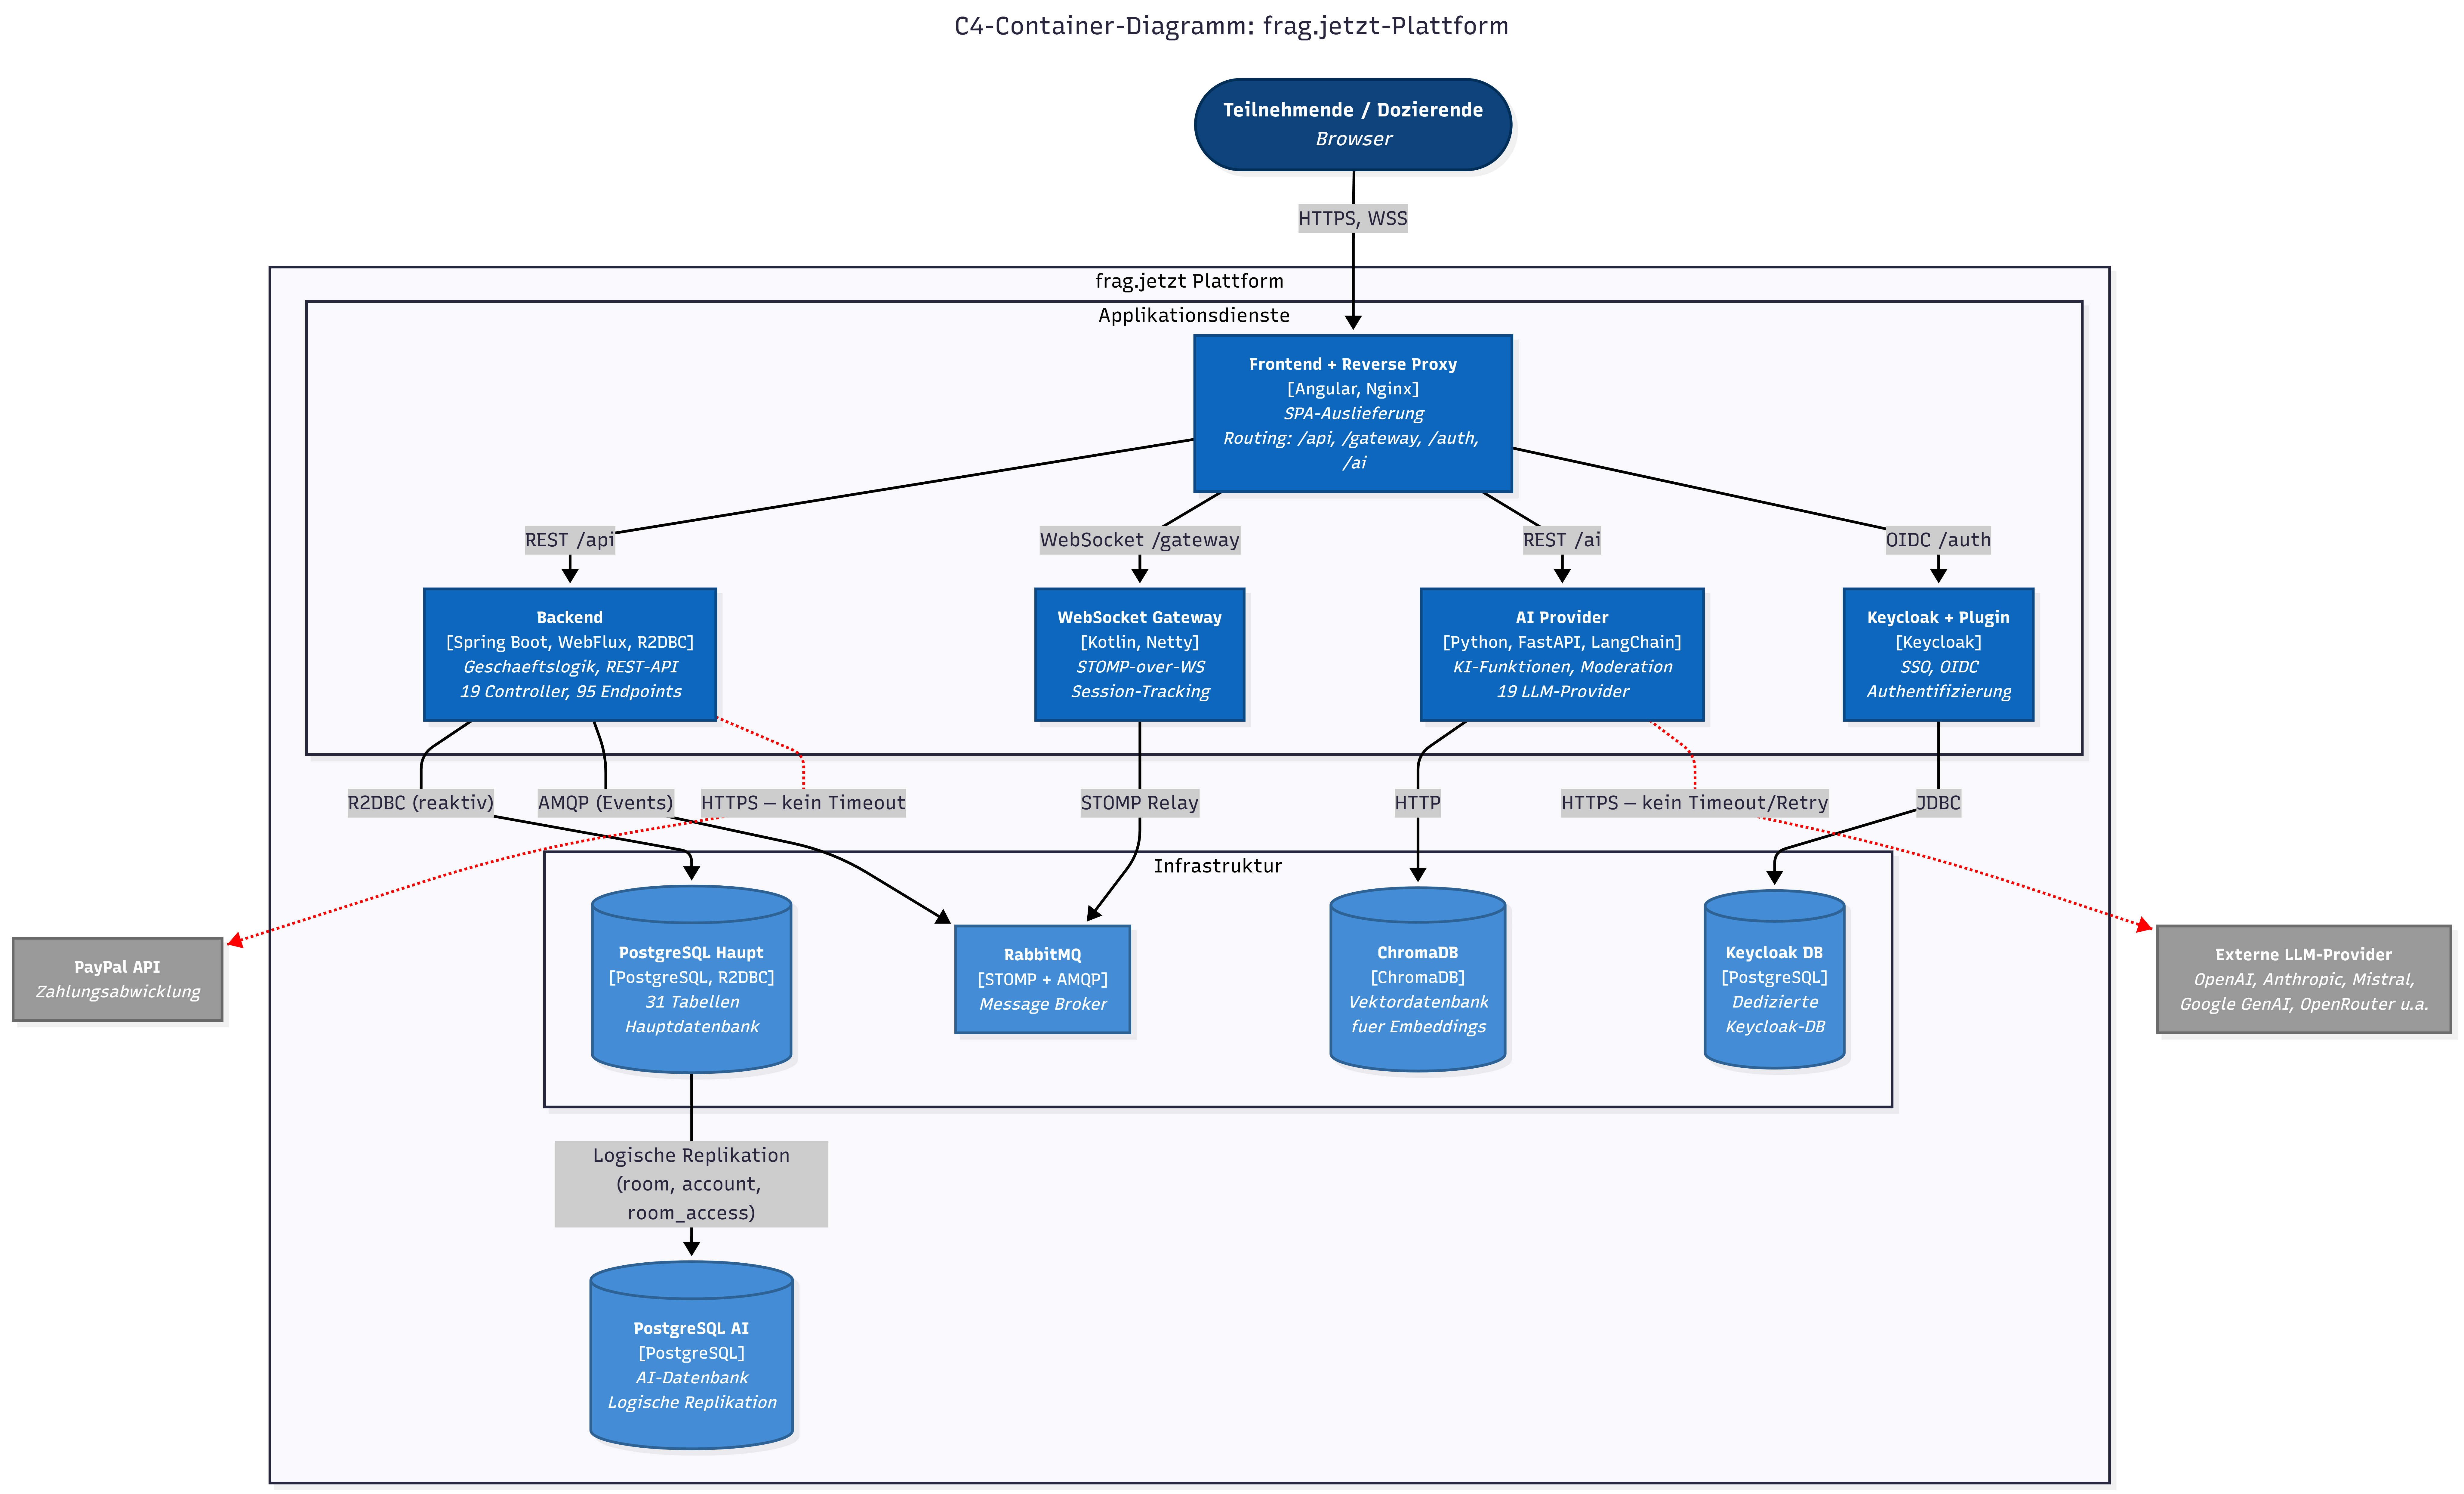
\includegraphics[angle=90,height=0.75\textheight,keepaspectratio]{images/frag.jetzt C4-Container-Diagram.png}
\caption{C4-Container-Diagramm der frag.jetzt-Architektur in Vollseitenansicht}
\label{fig:c4-fragjetzt-architektur-vollseite}
\end{figure}

 
\clearpage%
\printGenerativeAIDeclaration%
\clearpage%
\printDeclarationOfIndependence%
 
\end{document}